\chapter{Results}
\label{results}
%Looking also at the general picture usually helps, for example, looking at figure \ref{heatmap}, it is clear that way more paths ended up hitting the lights on the ceiling and on the staircase rather than the two light portals down the hall

Assessing the validity of a tool without performing user tests is often pointless but, due to the complexity of the tool, there was no time to perform any. In their absence, the analysis of two couples of significant datasets are presented.

\section{First dataset couple}

\begin{figure}
	\centering
	\begin{subfigure}[t]{0.49\linewidth}
		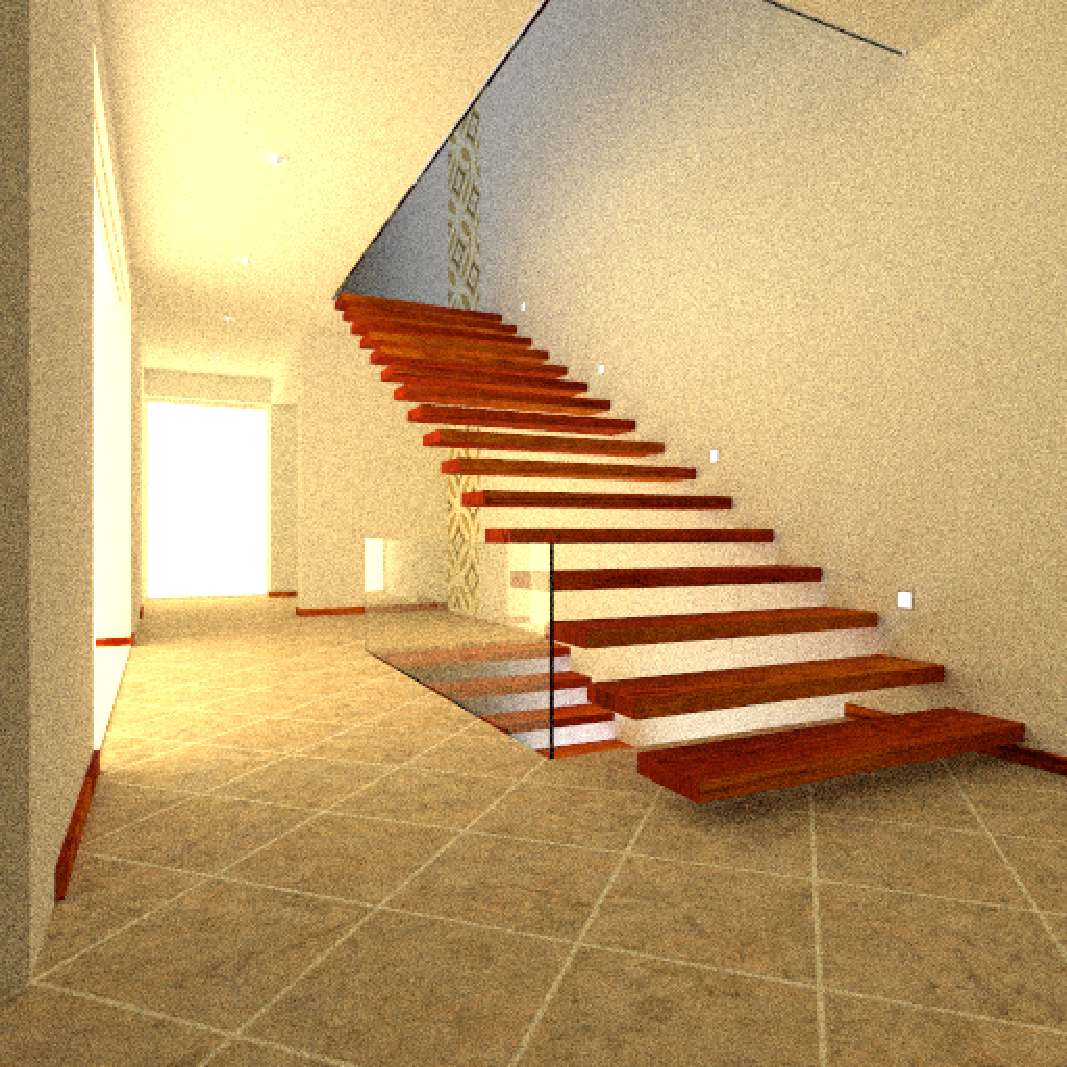
\includegraphics[width=\textwidth]{chapters/chapter_results/a_render.pdf}
		\caption{Render \texttt{A}}
	\end{subfigure}
	\begin{subfigure}[t]{0.49\linewidth}
		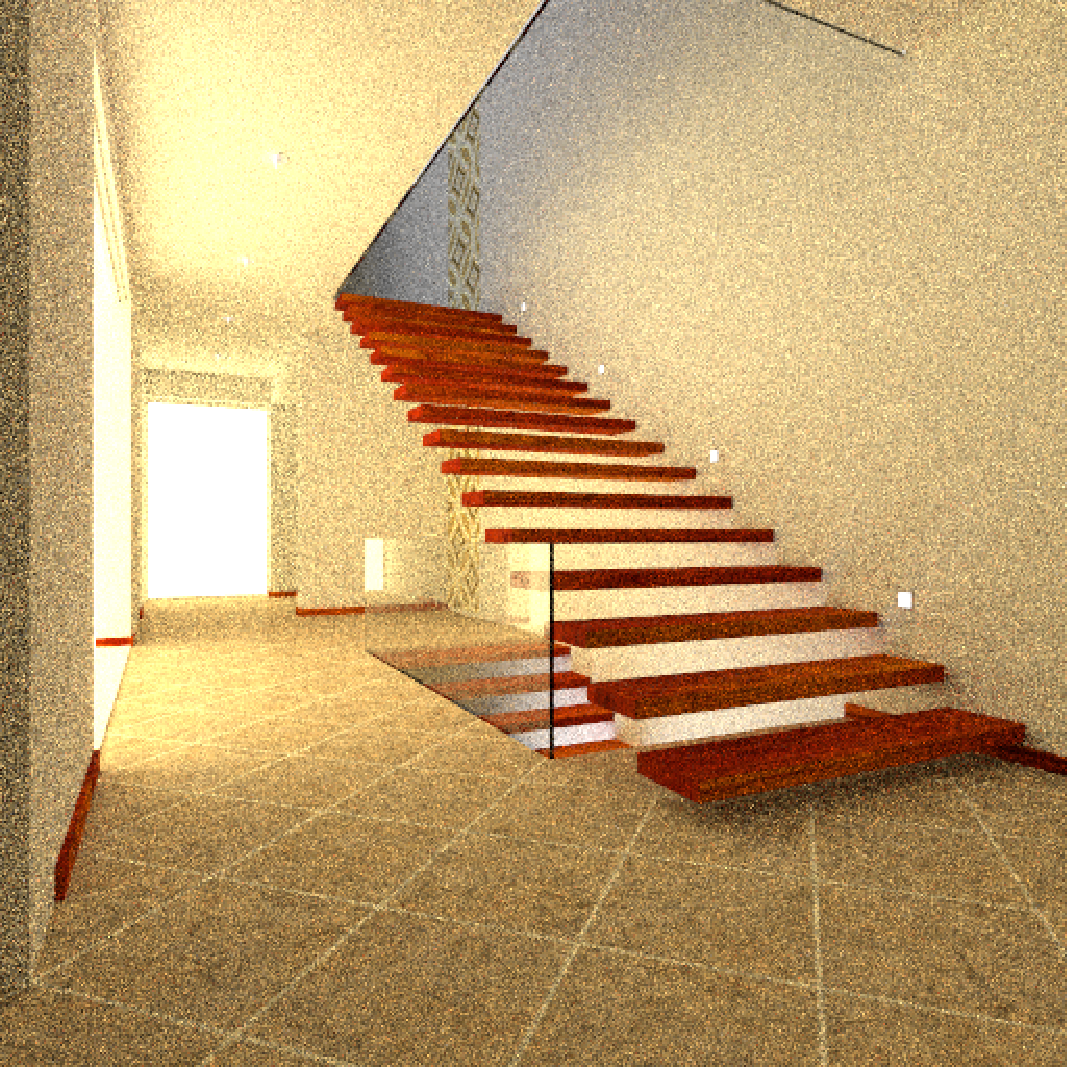
\includegraphics[width=\textwidth]{chapters/chapter_results/b_render.pdf}
		\caption{Render \texttt{B}}
	\end{subfigure}

	\caption{Render images of the two datasets.}
	\label{couple1render}
\end{figure}

The first example we are analyzing consists in comparing two datasets generated by Yocto/GL \cite{pellacini2019yocto} on the \textit{Modern Hall} scene \cite{bitterliscenes} with same resolution and same number of samples per pixel --- $512 \times 512$ and 256 spp --- but they are using different next event estimation techniques. The algorithm behind dataset \texttt{A} is using importance sampling based on the surface materials only, while the one behind dataset \texttt{B} is using multiple importance sampling on both surface materials and scene light sources. Given this, by intuition, the final render of dataset \texttt{B} should be less noisy than the one of dataset \texttt{A} but, as pictured in figure \ref{couple1render}, it is actually the opposite. Exploiting the features of the presented tool, we will now illustrate the reason behind this. 

\begin{figure}
	\centering
	\begin{subfigure}[t]{0.49\linewidth}
		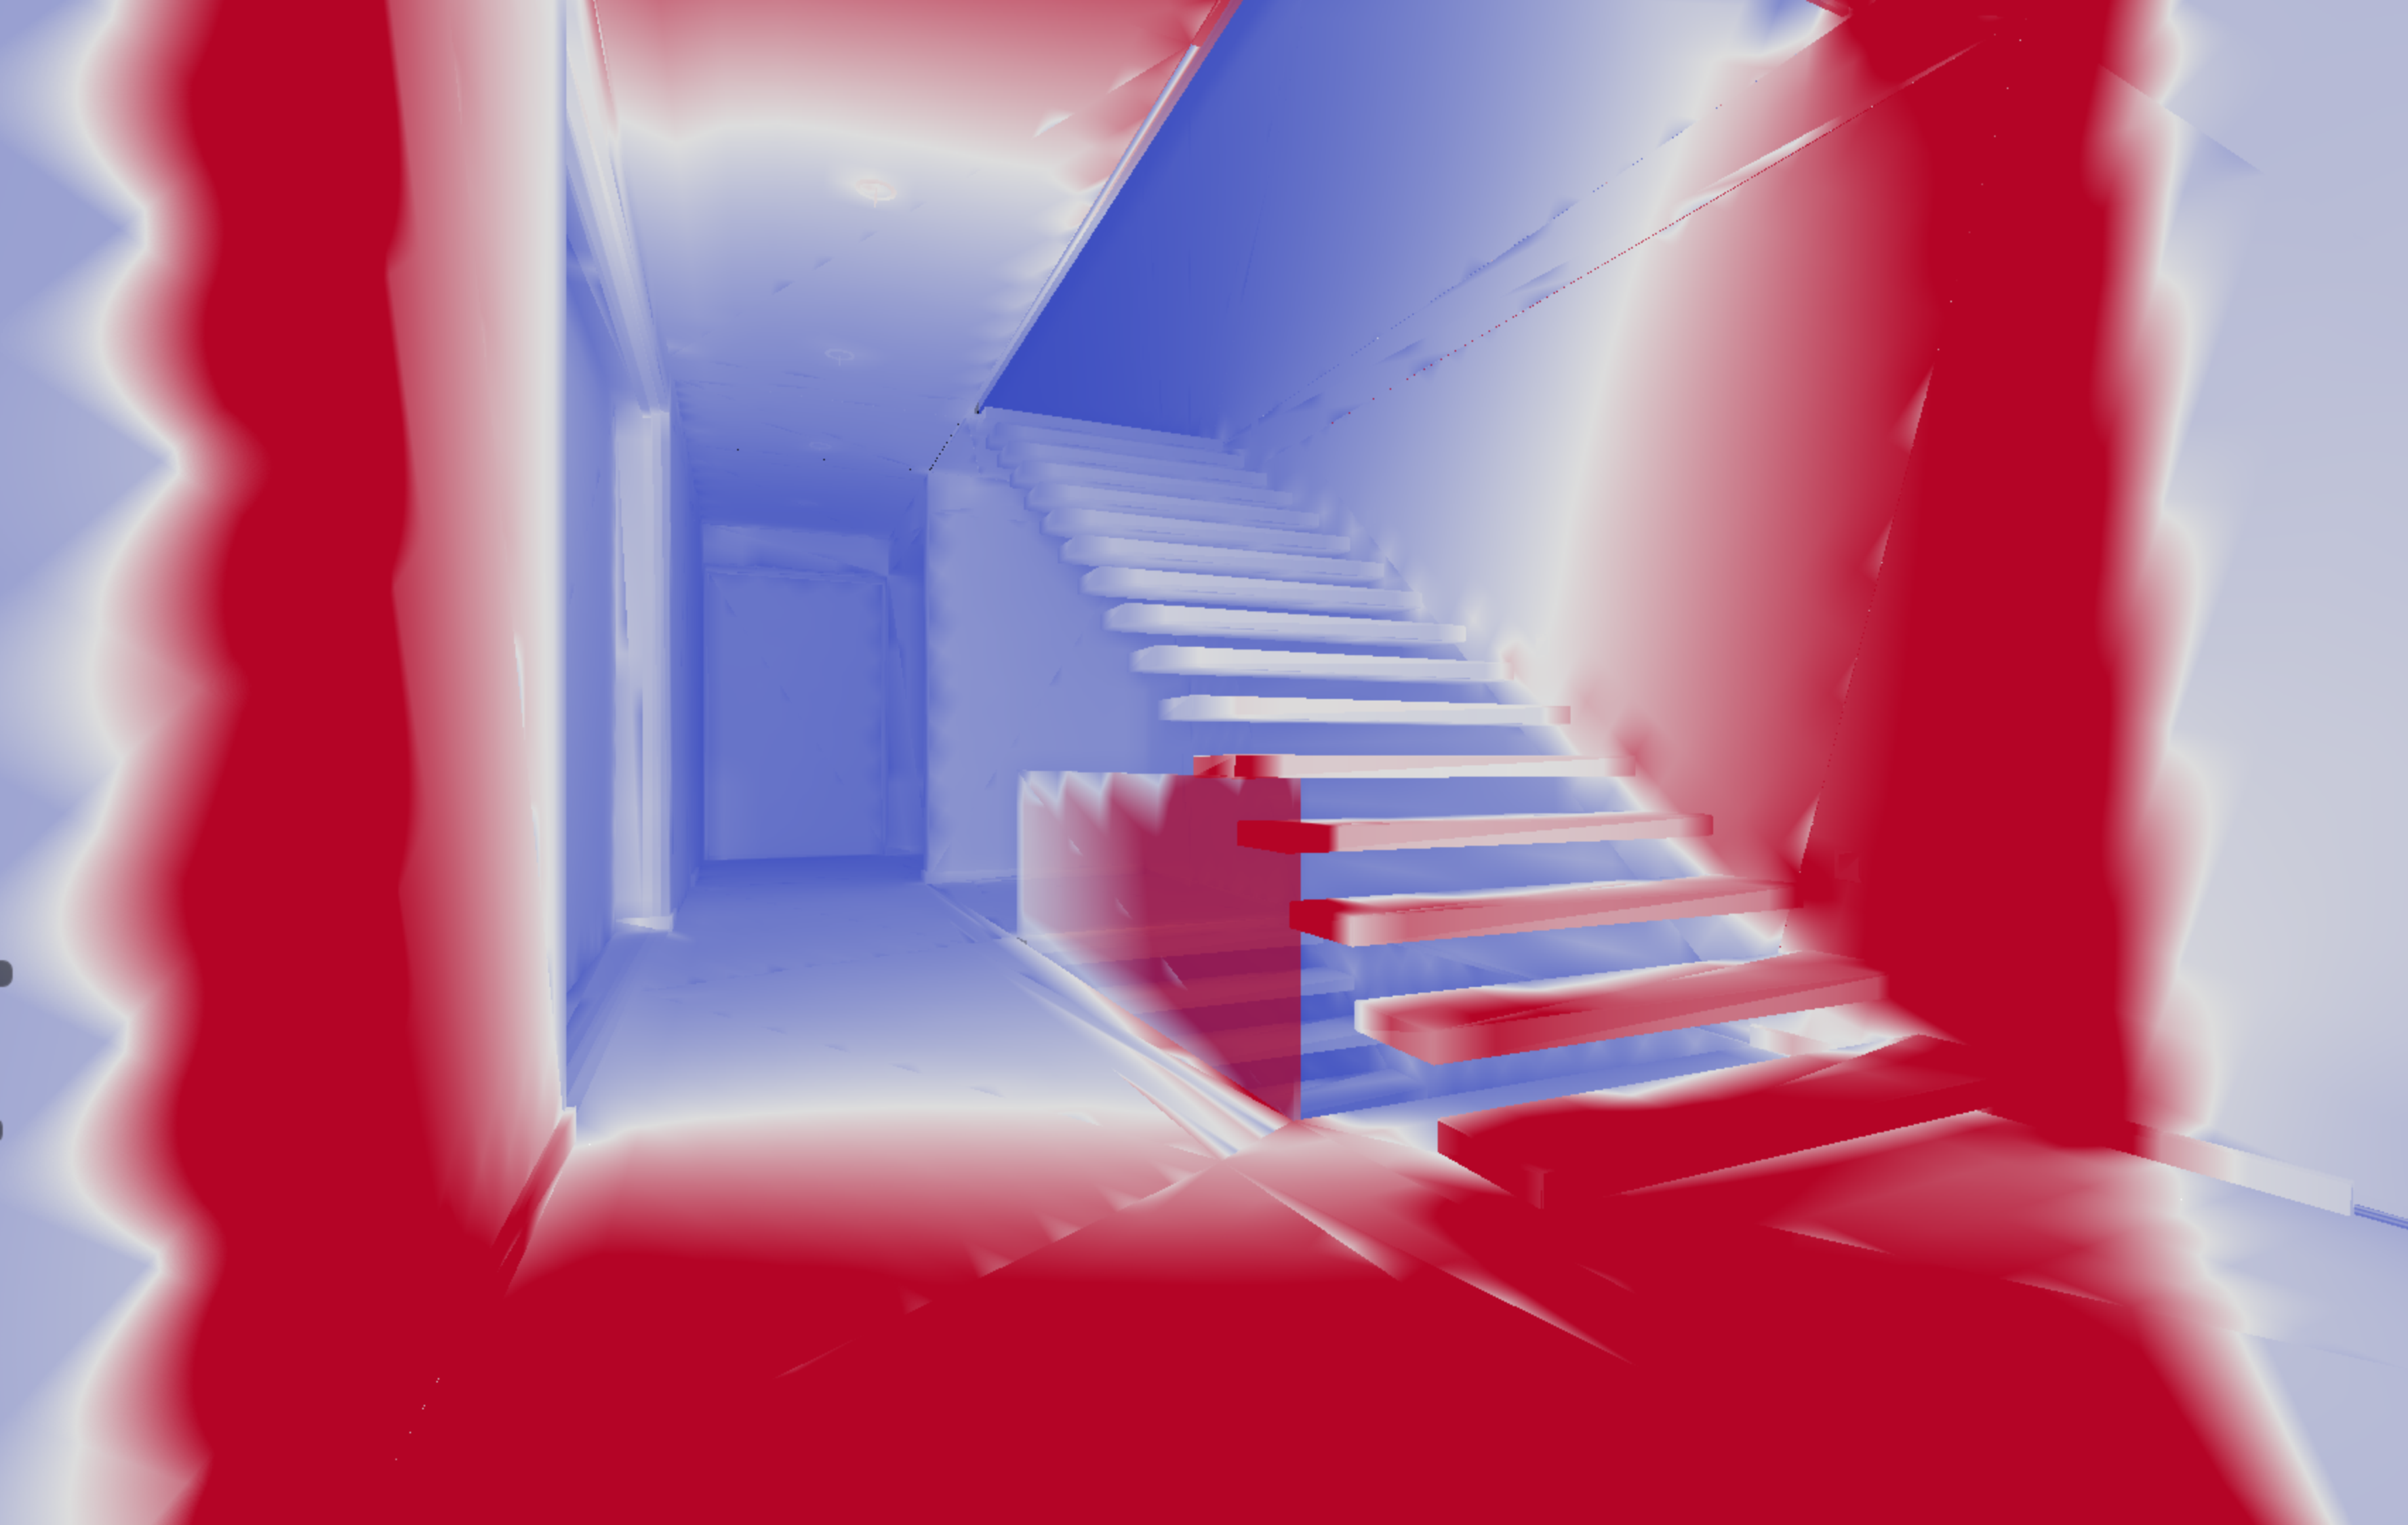
\includegraphics[width=\textwidth]{chapters/chapter_results/a_heatmap1}
		\caption{Dataset \texttt{A} heatmap 1}
	\end{subfigure}
	\begin{subfigure}[t]{0.49\linewidth}
		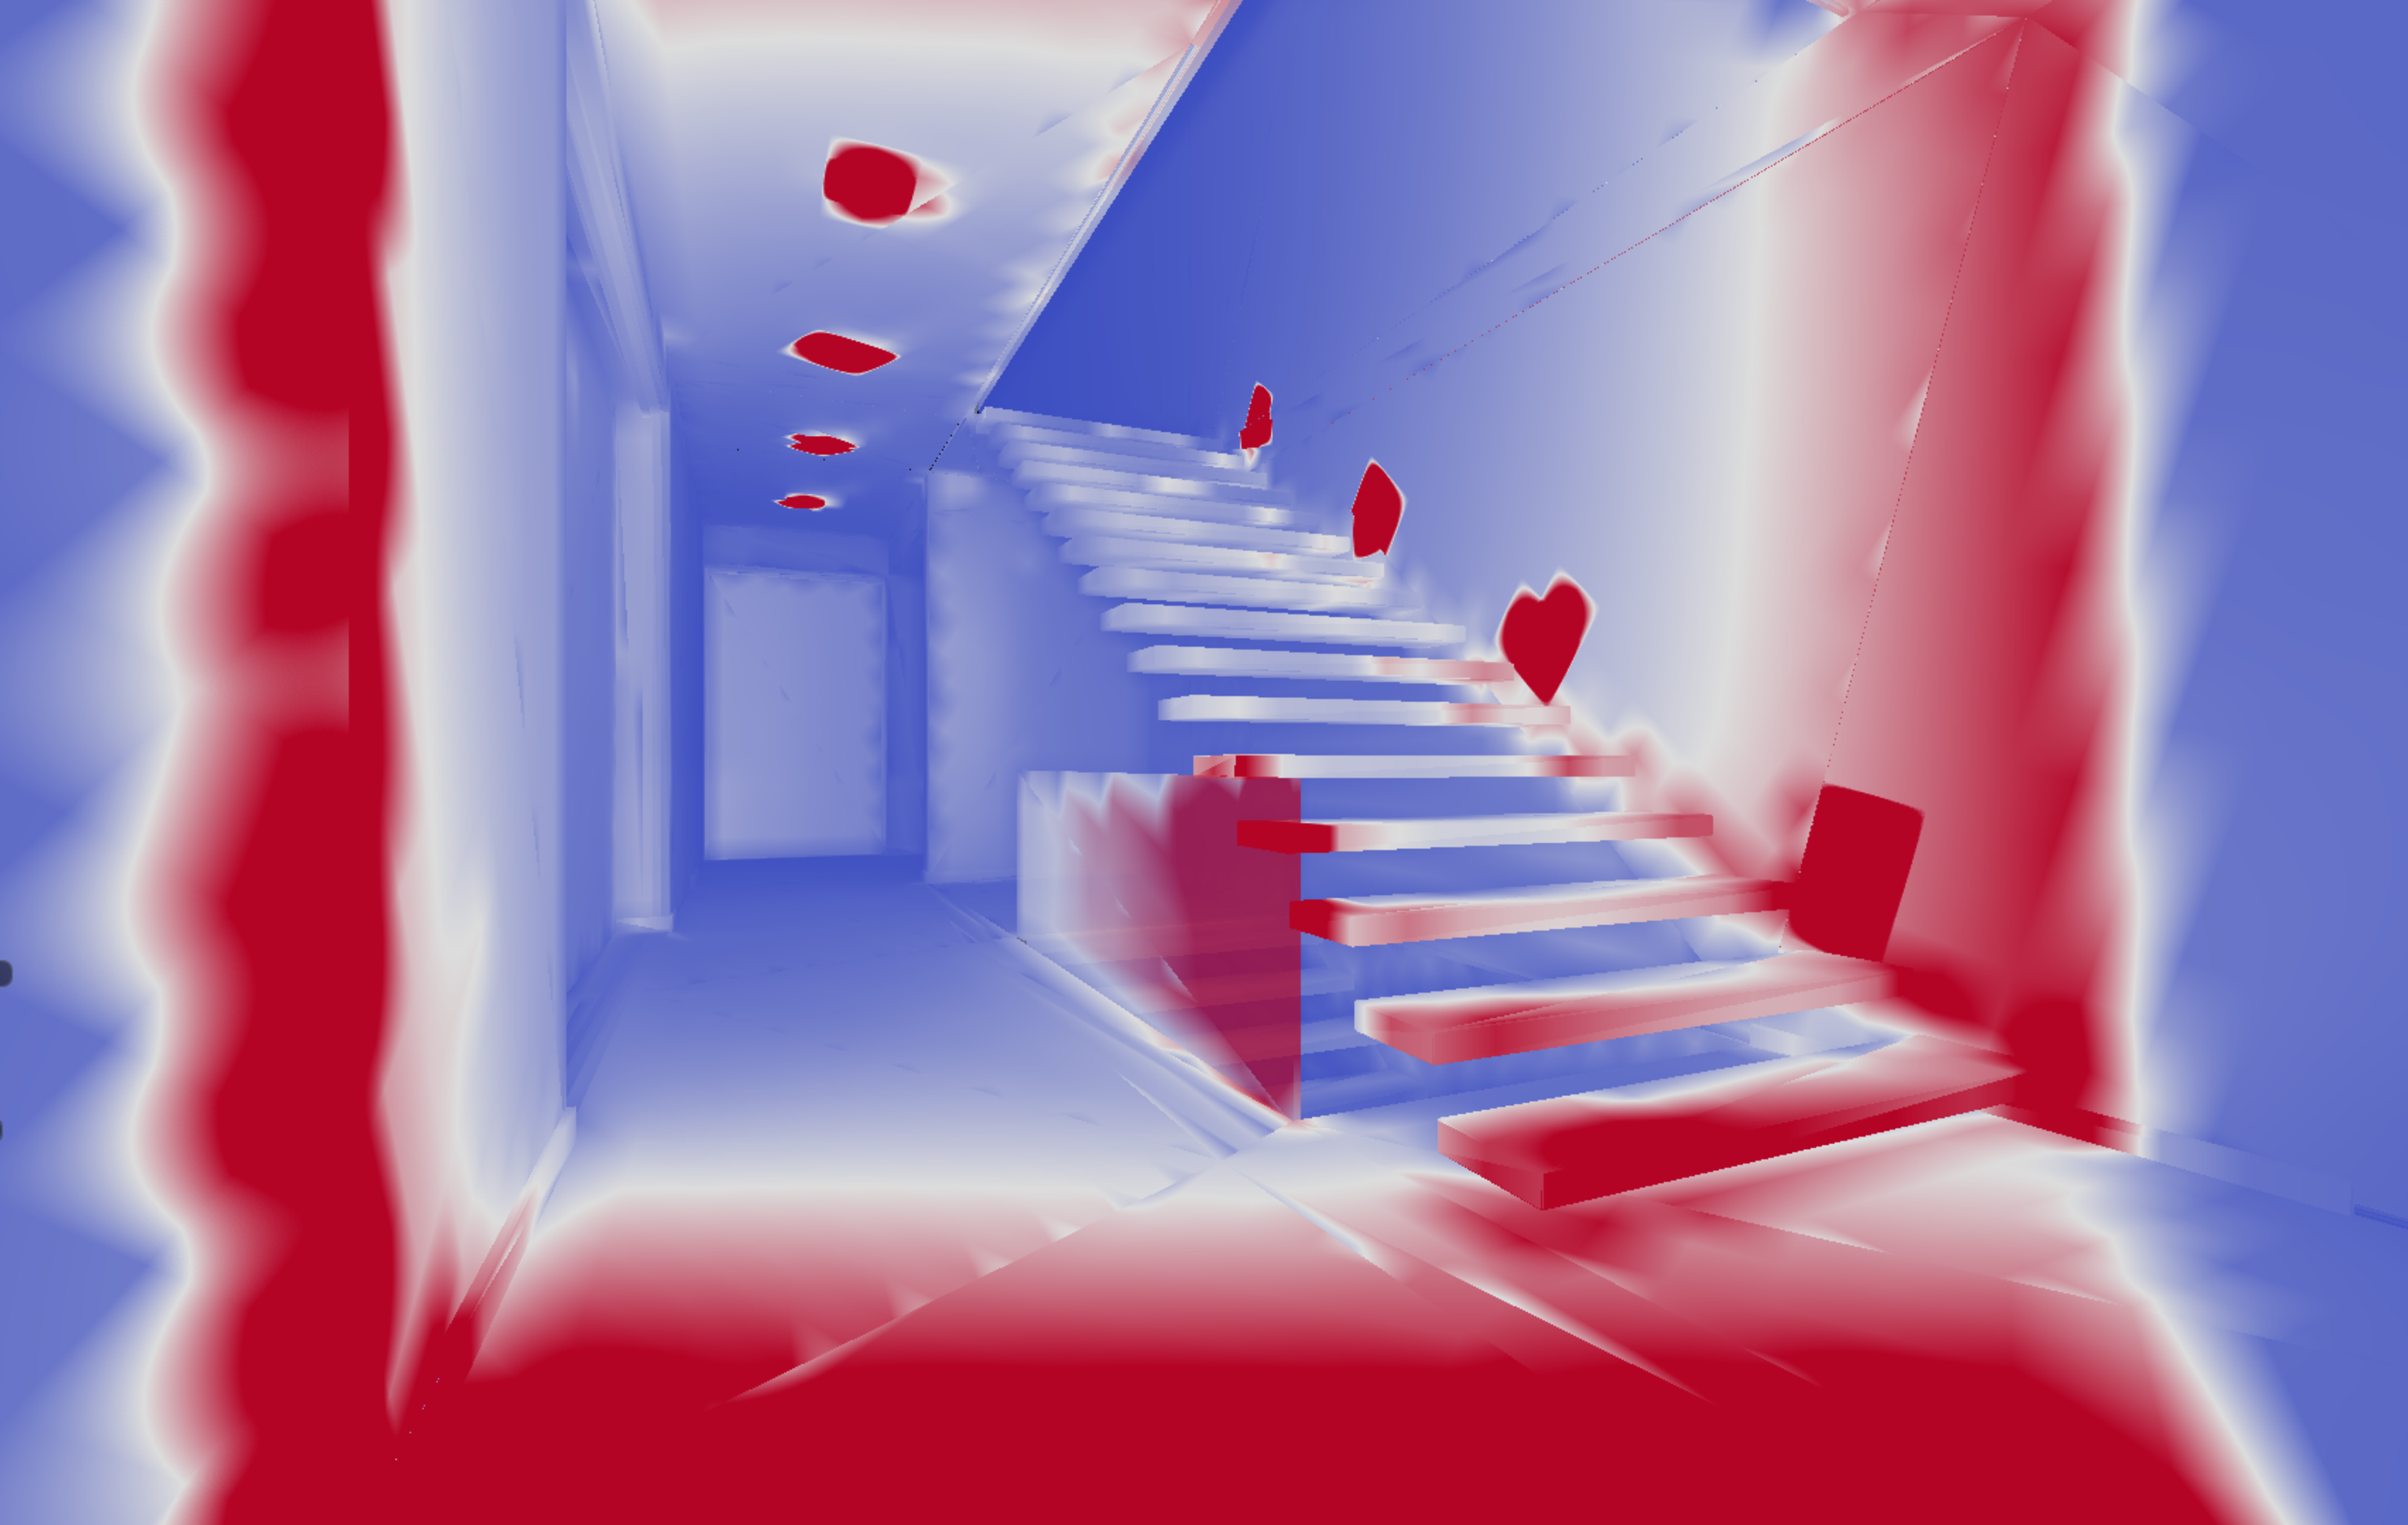
\includegraphics[width=\textwidth]{chapters/chapter_results/b_heatmap1}
		\caption{Dataset \texttt{B} heatmap 1}
	\end{subfigure}
	\begin{subfigure}[t]{0.49\linewidth}
		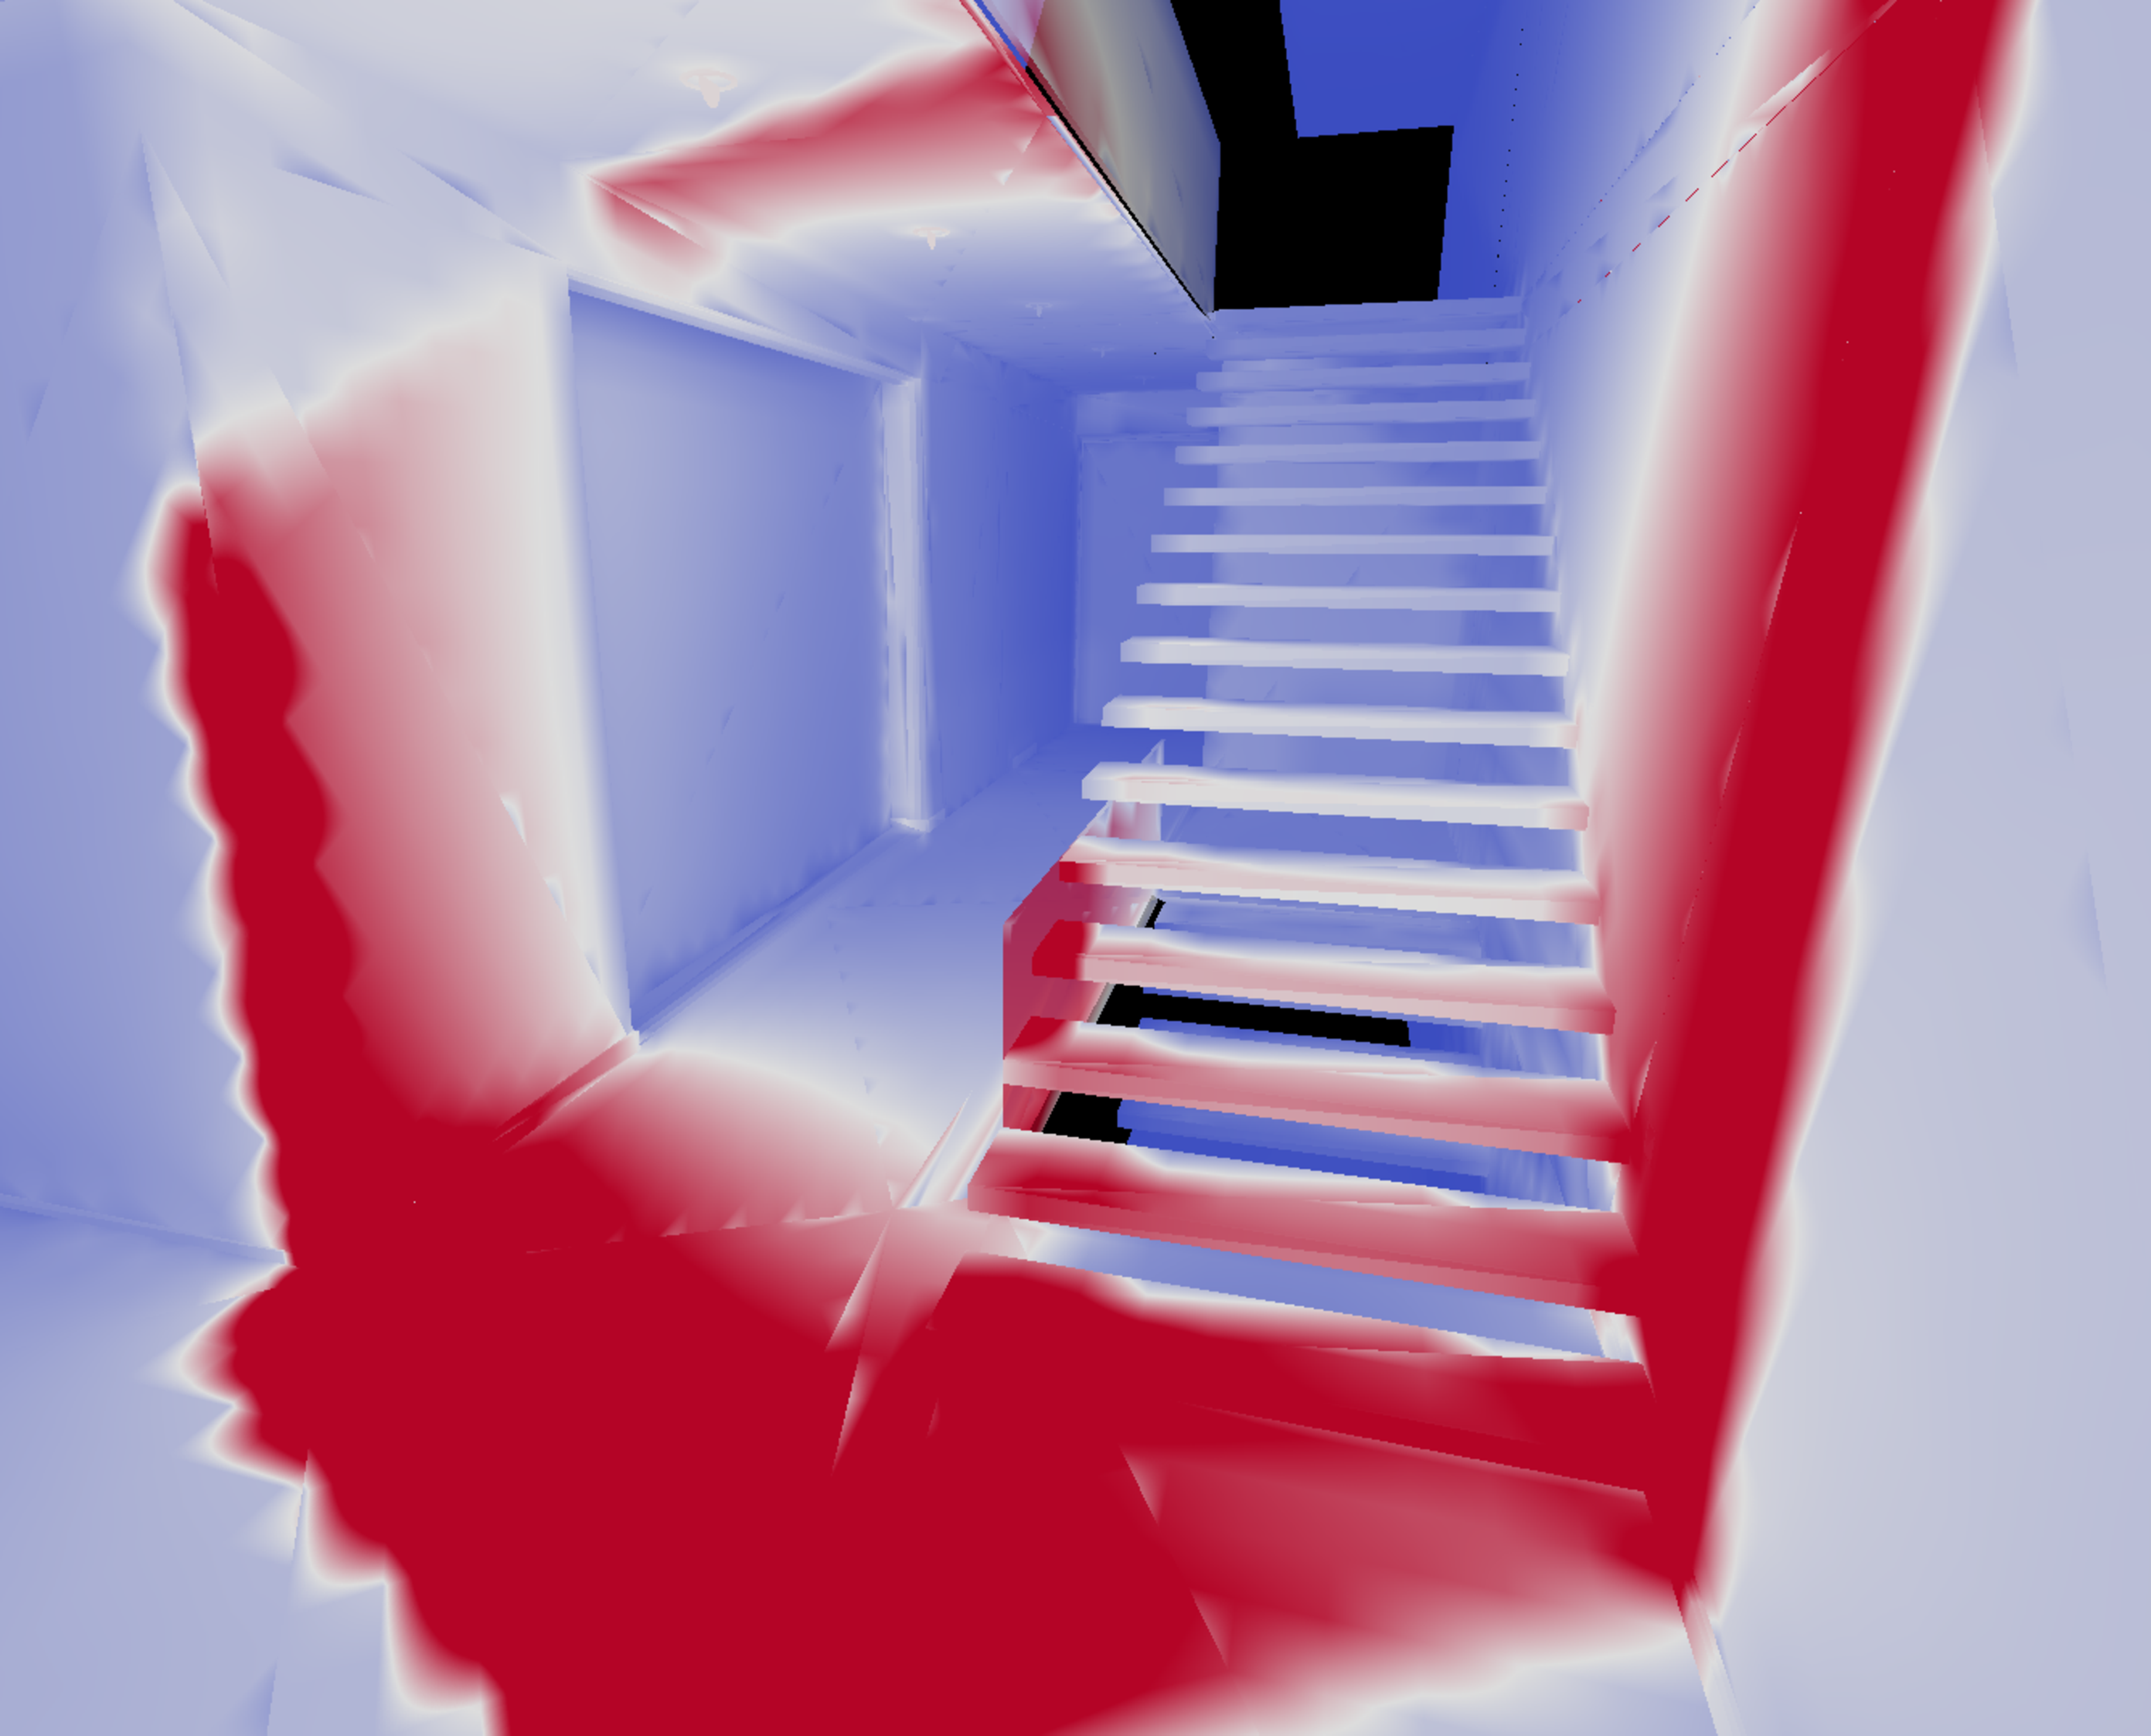
\includegraphics[width=\textwidth]{chapters/chapter_results/a_heatmap2}
		\caption{Dataset \texttt{A} heatmap 2}
	\end{subfigure}
	\begin{subfigure}[t]{0.49\linewidth}
		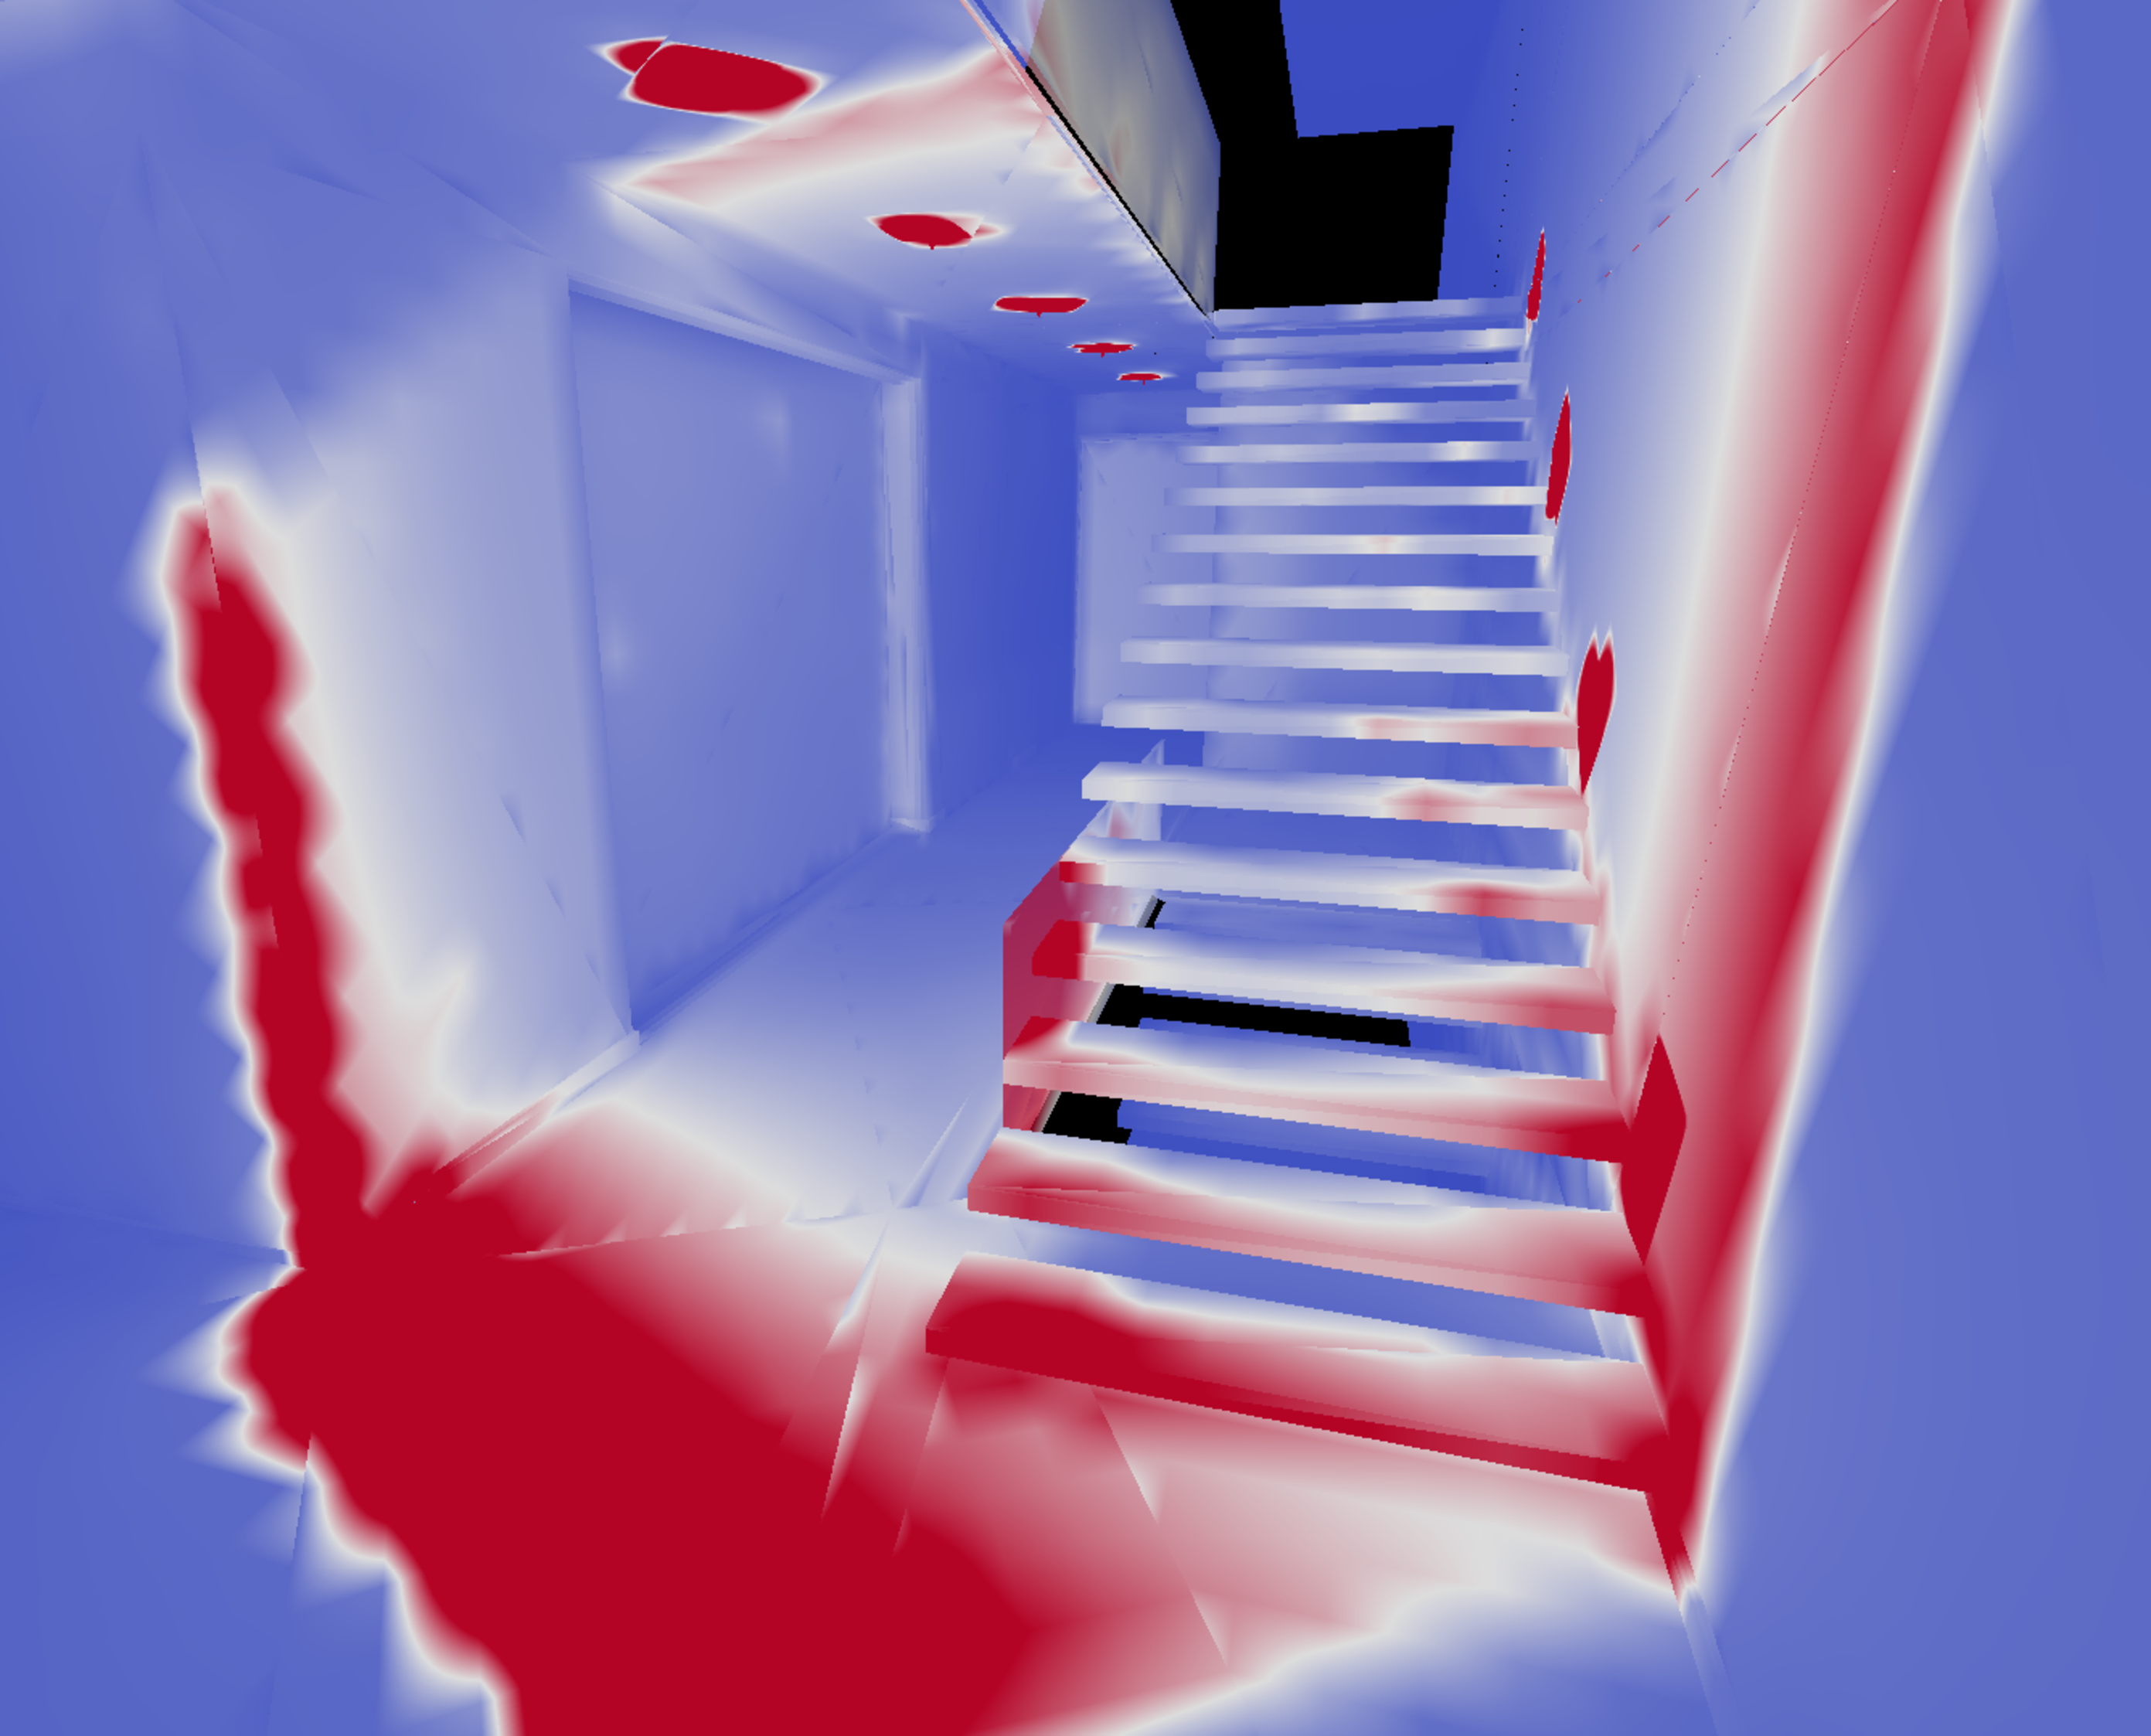
\includegraphics[width=\textwidth]{chapters/chapter_results/b_heatmap2}
		\caption{Dataset \texttt{B} heatmap 2}
	\end{subfigure}

	\caption{Heatmap renderings for both datasets from two different cameras. \textbf{“Heatmap max”} parameter has been set to $200,000$ for both.}
	\label{couple1heatmaps}
\end{figure}

\begin{figure}
	\centering
	\begin{subfigure}[t]{0.2\linewidth}
		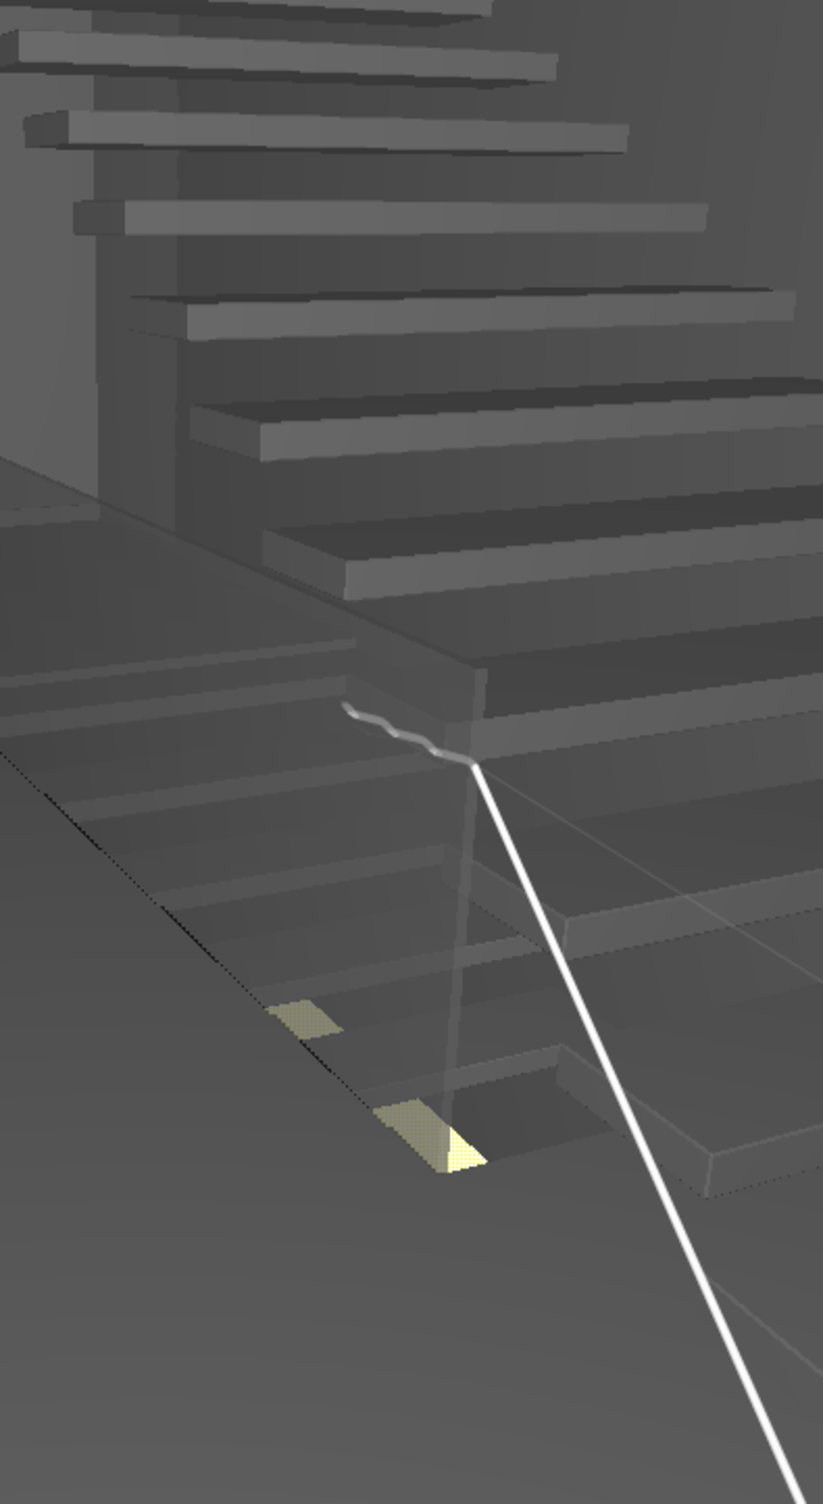
\includegraphics[width=\textwidth]{chapters/chapter_results/opticfiber_ext}
		\caption{ }
	\end{subfigure}
	\begin{subfigure}[t]{0.79\linewidth}
		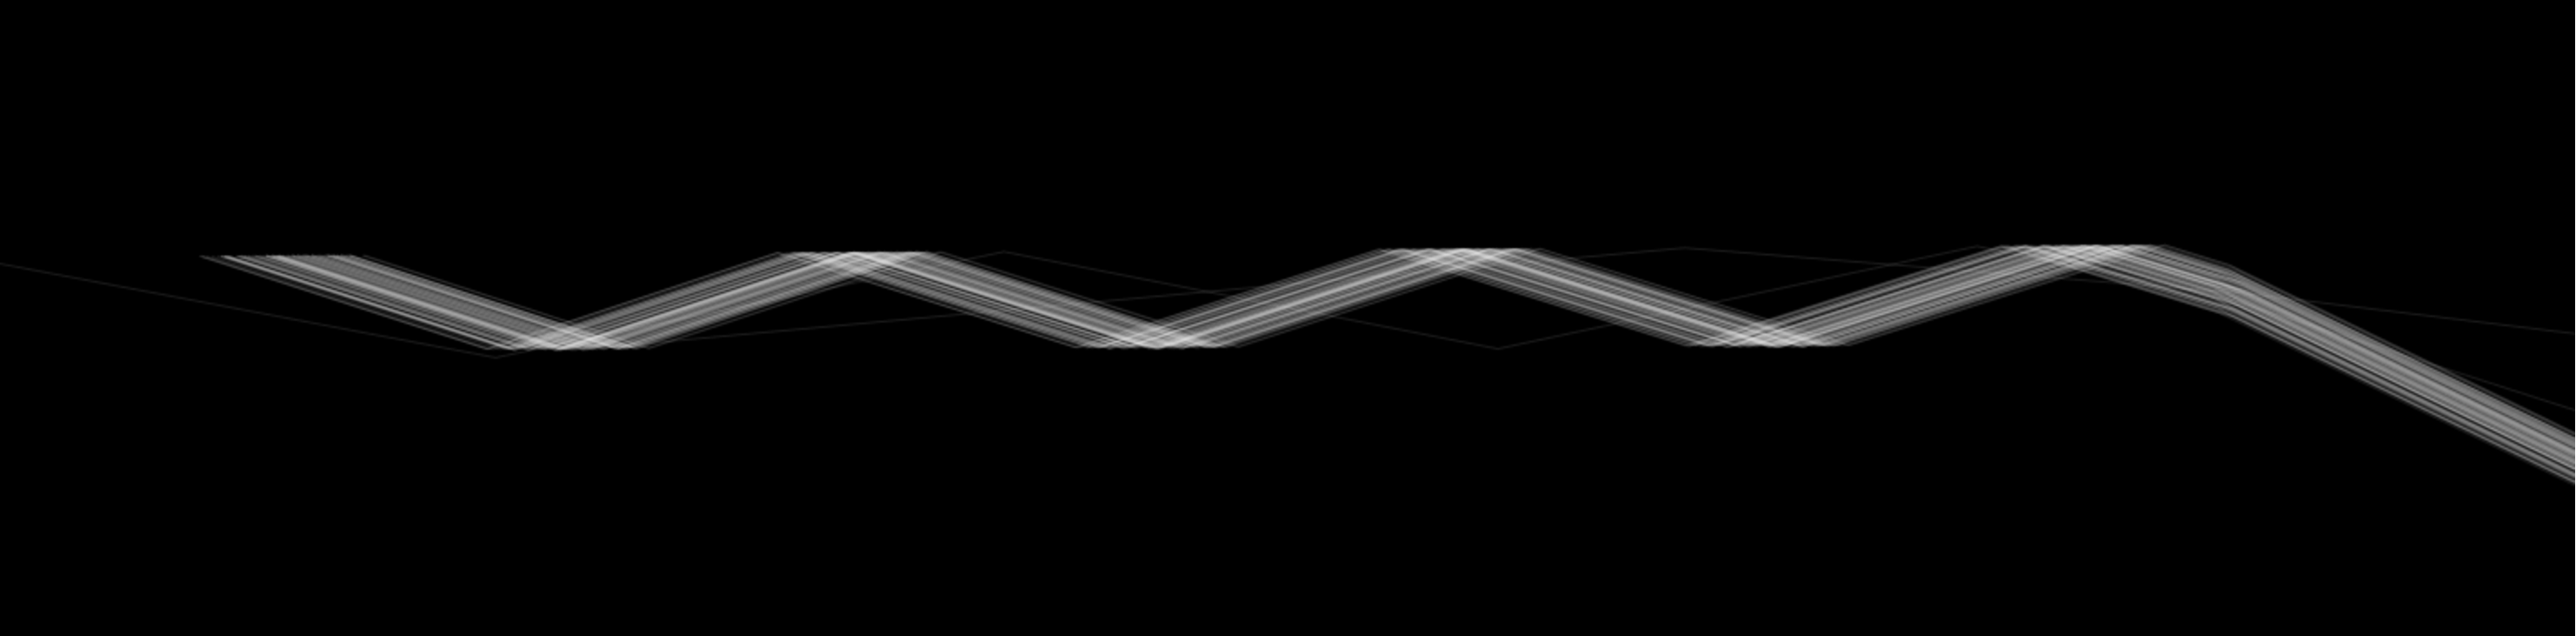
\includegraphics[width=\textwidth]{chapters/chapter_results/opticfiber}
		\caption{ }
	\end{subfigure}

	\caption{Viewport renders of a hundred of paths bouncing inside the glass panel, demonstrating the total internal reflection phenomenon. (\textbf{b}) is taken from above with all geometries hidden. Please note also how the paths bend upon entering the glass surface on the extreme right of (\textbf{b}).}
	\label{opticfiber}
\end{figure}

Bounce density heatmap visualization (fig. \ref{couple1heatmaps}) clearly shows the effects of importance sampling: please notice how the most bounce-dense areas in dataset \texttt{B} are localized on the lights on the ceiling and near the stairs and how the glass panel tends to be redder than its surroundings in both datasets. While the former shows how the paths of dataset \texttt{B} tends to go towards the light in the scene, the latter is a direct manifestation of the total internal reflection phenomenon; paths that enter the glass pane from its narrower side --- the one closer to the camera --- gets trapped inside the glass and keep bouncing on the internal glass surface (fig. \ref{opticfiber}) as similarly as it happens inside an optic fiber cable. This would be possible only when performing next event estimation based on the surface material properties: without accounting the index of refraction of glass while generating new directions after the bounces, a path tracer would not be able to reproduce this phenomenon. Even though this is an interesting result, it does not entirely explain why a render clearly done using multiple importance sampling has more noise that the one without this feature. A hint is there though: as already noted, a copious amount of paths of dataset \texttt{B} bounced on the tiny lights on the ceiling and next the stairs, even if this is normal for this kind of algorithm, it gets worrying when noticed that the scene is almost entirely illuminated by the two warm light portals on the corridor and the two cold ones down and up the stairs; the tiny lights where all those paths ended up to do not contribute at all at the global illumination of the scene. This means that every path that ends up on those lights will carry very little radiance compared to the ones that reach the portal lights, introducing noise in the final render. But let us analyze this further.

\begin{figure}
	\centering
	\begin{subfigure}[t]{0.32\linewidth}
		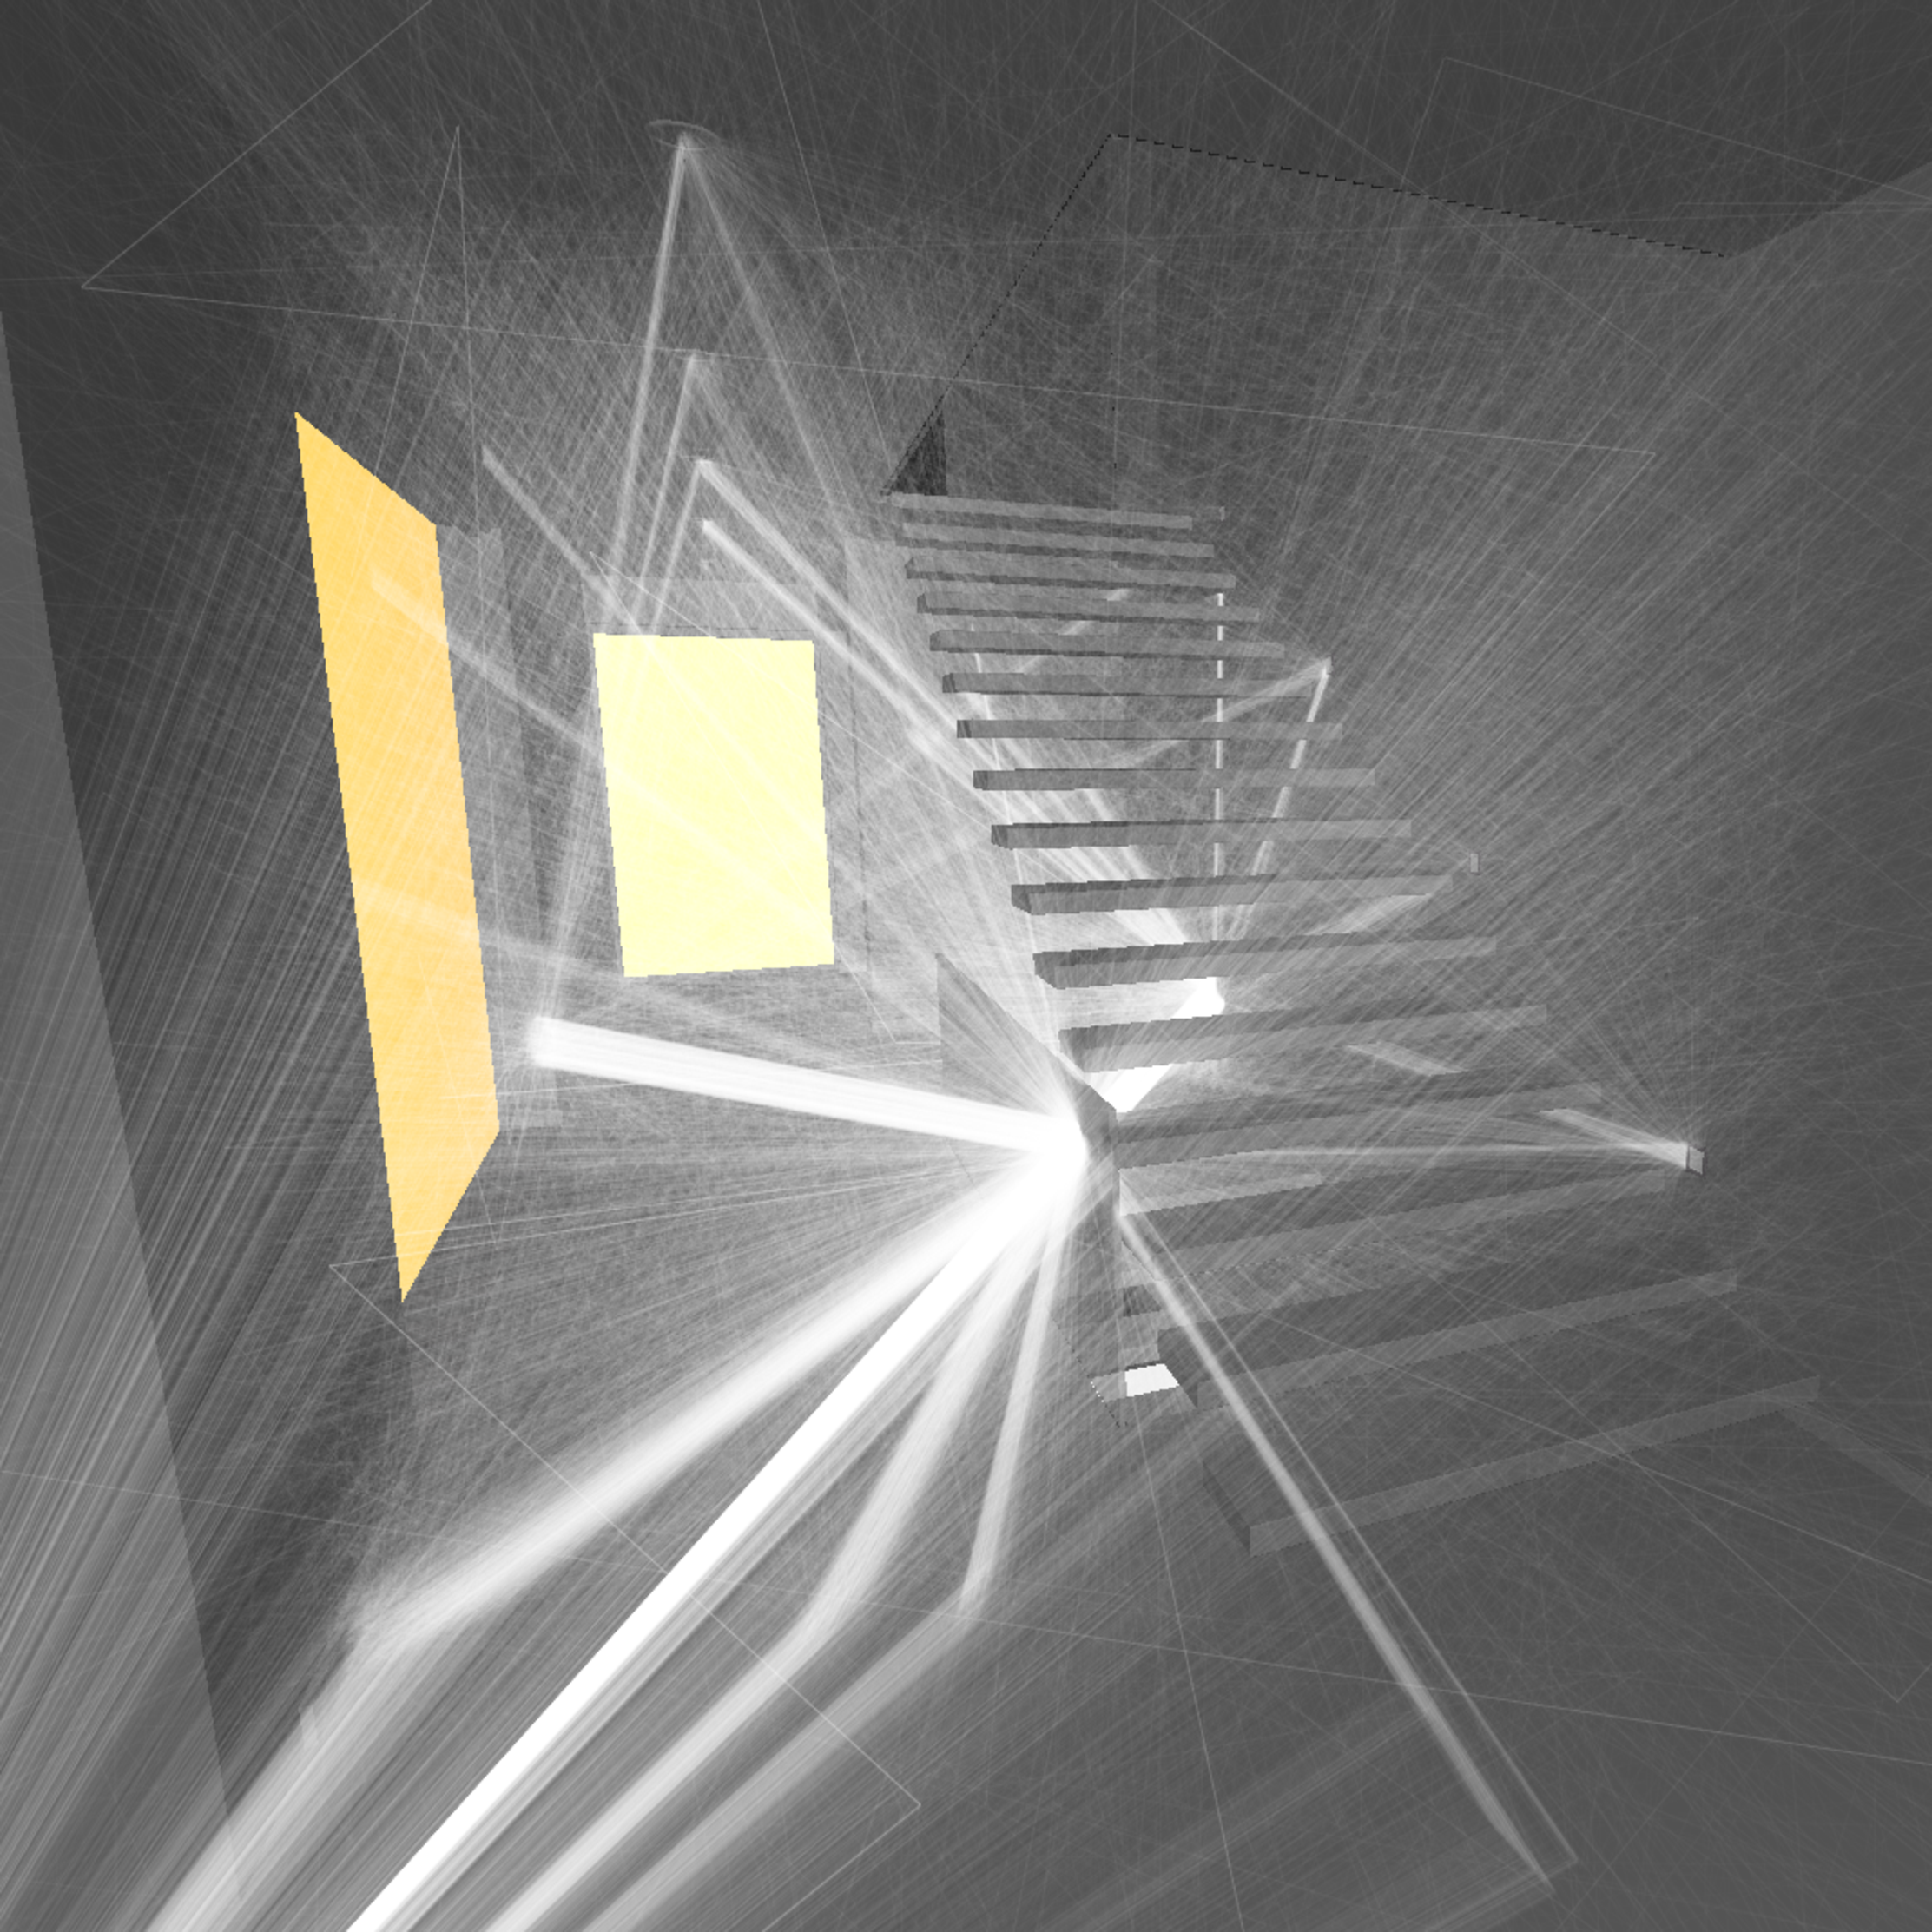
\includegraphics[width=\textwidth]{chapters/chapter_results/b_paths1}
		\caption{Viewport}
		\label{b_paths1}
	\end{subfigure}
	\begin{subfigure}[t]{0.32\linewidth}
		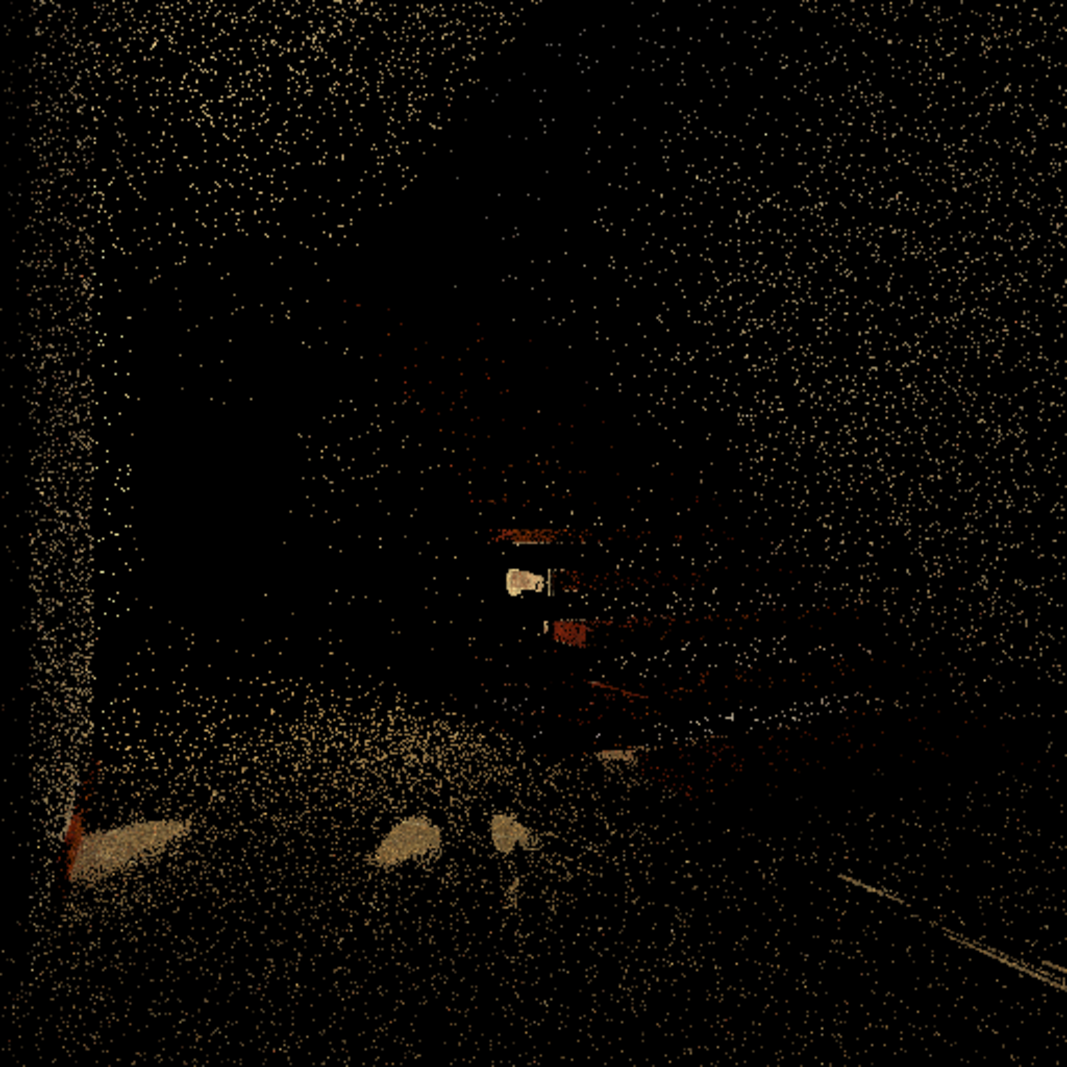
\includegraphics[width=\textwidth]{chapters/chapter_results/b_image1}
		\caption{\textbf{“Final radiance”} viz}
	\end{subfigure}
	\begin{subfigure}[t]{0.32\linewidth}
		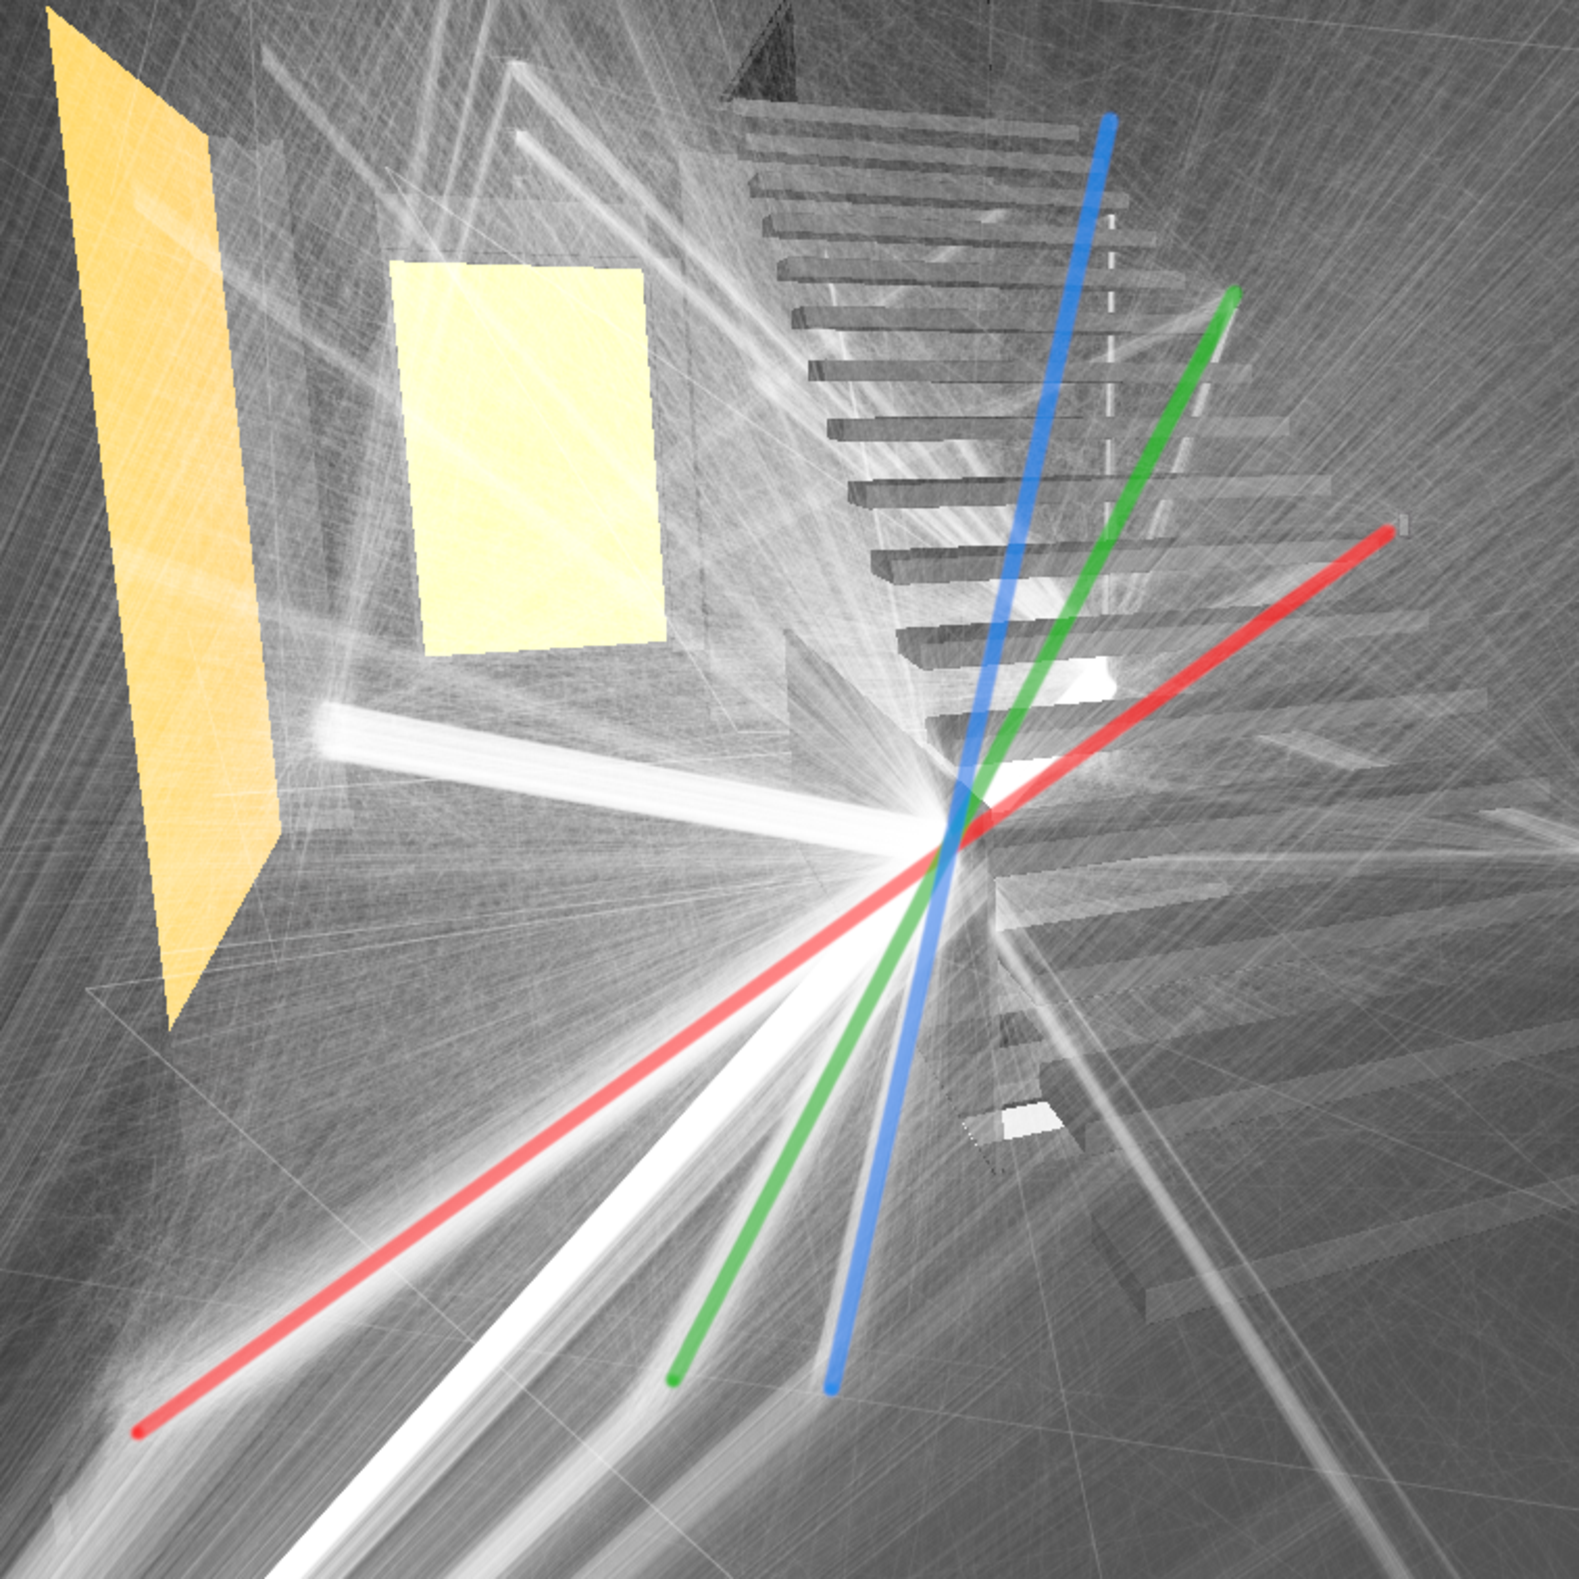
\includegraphics[width=\textwidth]{chapters/chapter_results/b_paths1highlight}
		\caption{Bundles detail}
		\label{b_paths1highlight}
	\end{subfigure}

	\caption{Visualizations of the paths selected by a sphere filter placed on the glass panel for dataset \texttt{B}. (\textbf{a}) shows a viewport render, (\textbf{b}) is the view available in the \textbf{“Image”} panel with the \textbf{“Final radiance”} visualization mode selected (sec. \ref{image_widget}), and (\textbf{c}) shows highlighted in red, green, and blue three paths bundles and how they were directed to three light sources but have been occluded by the glass panel.}
	\label{couple2paths1}
\end{figure}

By placing a sphere filter on a point on the glass panel and looking at how dataset \texttt{B} reacts, more information starts showing (fig. \ref{couple2paths1}). Many path bundles connecting various areas in the scene appear and it seems that, while most of these connect the camera, lights, and the filter between each other, there are some that apparently are not directly connected to any relevant point. But, after further inspection, it is clear that they are bundles of paths that try to reach a light source but can not since there are some other scene geometries sitting between the bundle and the light.
Please look, for example, at the three path bundles connecting the camera to the sphere filter while bouncing on the floor highlighted by figure \ref{b_paths1highlight} and how they do not seem to be connected to any light source directly; they are made of paths that have been directed towards the lights on the stairs but could not due to the glass panel standing in their way. We can coincidentally see them since our sphere filter sits on the portion of the glass panel in the way of those paths.

\begin{figure}
	\centering
	\begin{subfigure}[t]{0.49\linewidth}
		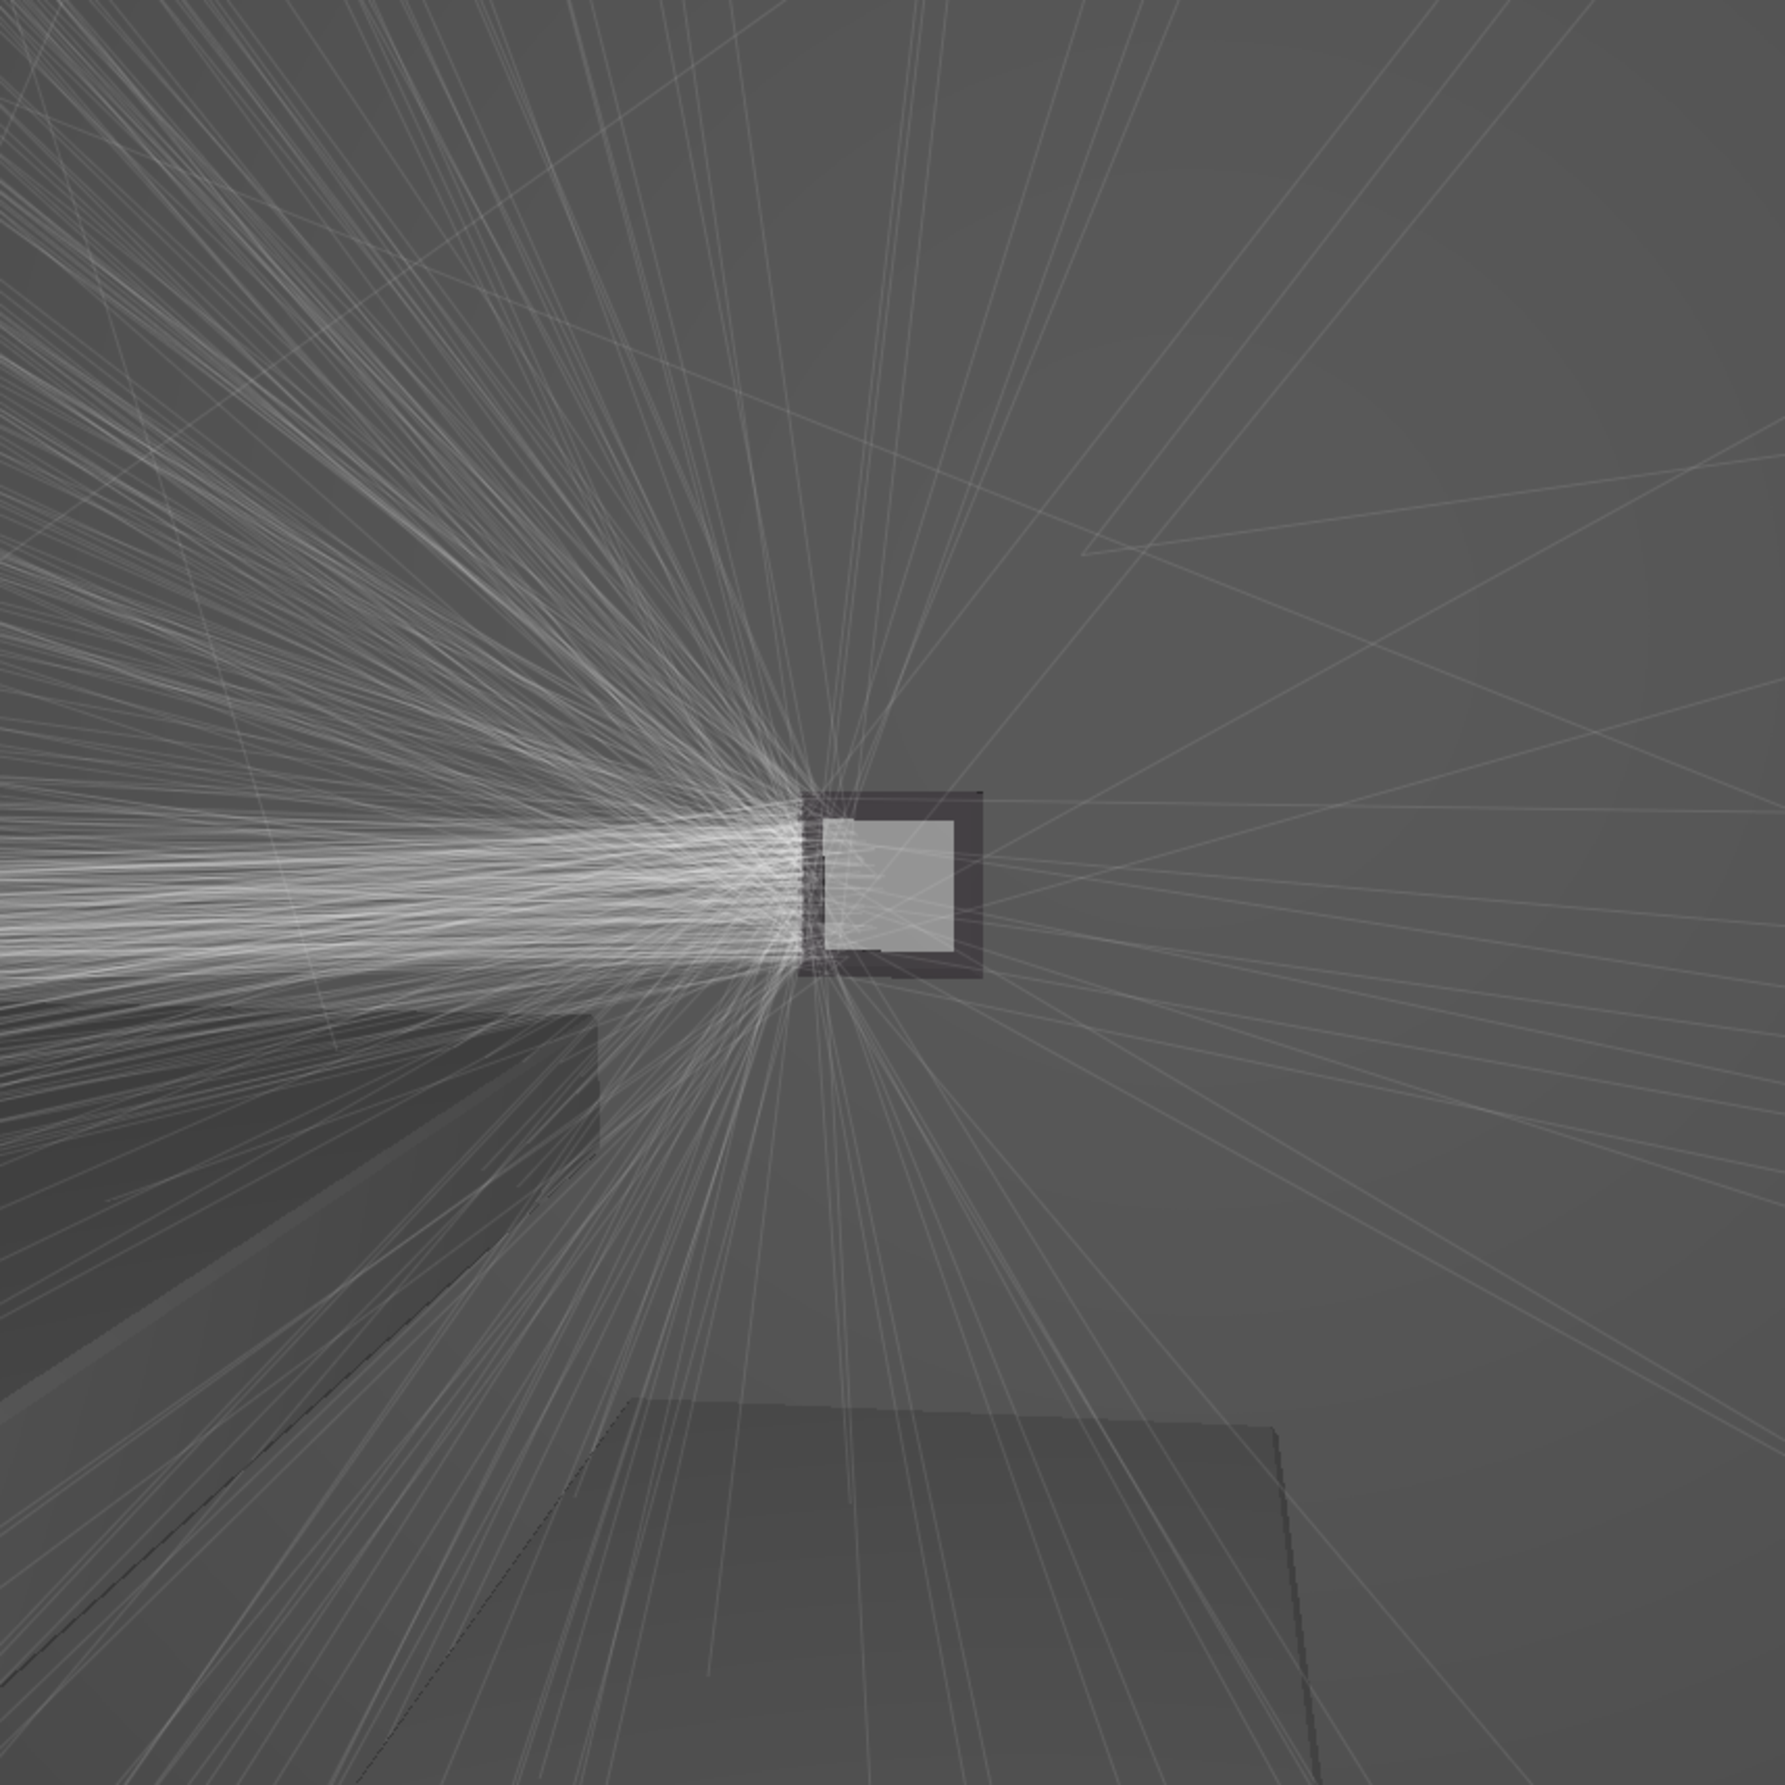
\includegraphics[width=\textwidth]{chapters/chapter_results/b_light}
	\end{subfigure}
	\begin{subfigure}[t]{0.49\linewidth}
		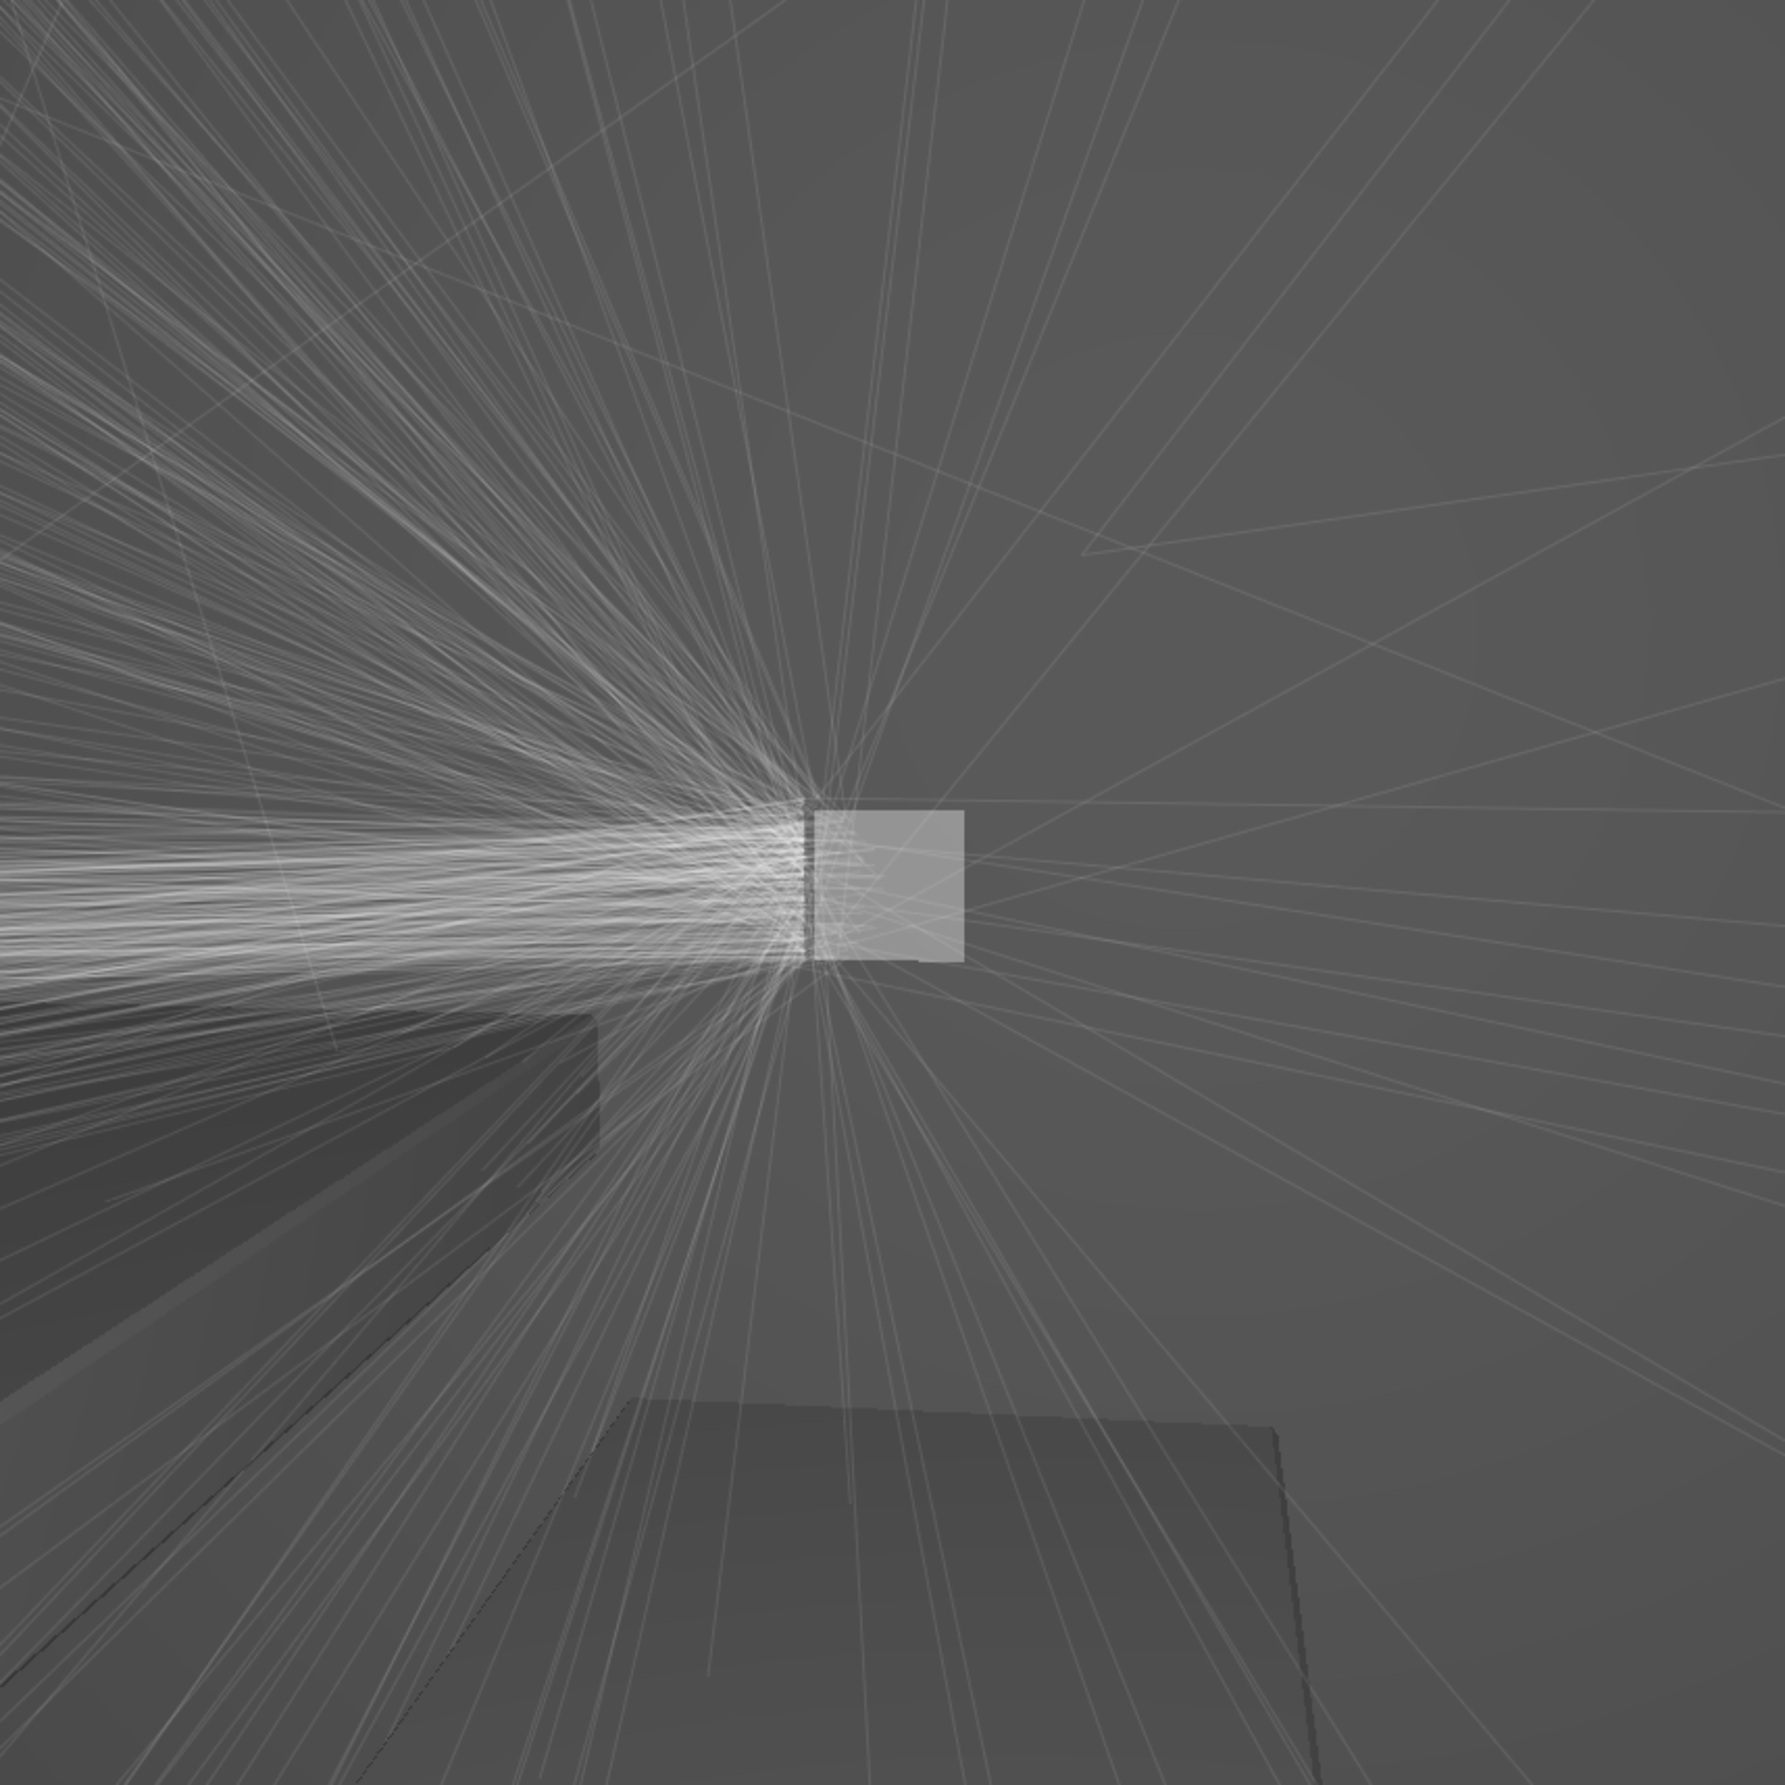
\includegraphics[width=\textwidth]{chapters/chapter_results/b_lightoff}
	\end{subfigure}

	\caption{Detail of the first stair light with the surrounding geometry shown on left and hidden on the right.}
	\label{couple2light}
\end{figure}

Looking at figure \ref{b_paths1} with more attention, more curious path bundles can be spotted: almost every light on the wall by the stairs has a bundle entering it while being almost parallel to the wall. A detail of the first stair light is presented in figure \ref{couple2light} and it can be seen that the bundle seems to hit the dark gray frame surrounding the light more that the light itself. Hiding the frame geometry in the viewport confirms the suspect: all those paths which have been shot in direction of the stair light are completely wasted since they are occluded by a frame. Furthermore, the frame seems to occlude a significant portion of the light surface making it unreachable by any path while still being a valid candidate for light sampling; in other words, the next event estimation will keep trying shooting paths on those surfaces hidden under the frame but will never reach them in any possible case, wasting energy and time.

To summarize, the render with multiple importance sampling over both the materials and the lights --- dataset \texttt{B} --- has more noise than the one sampling only against the materials --- dataset \texttt{A} --- because:
\begin{enumerate}
	\item The renderer, Yocto/GL, while sampling the light areas, gives the same weight to lights with a huge difference in intensity. This leads to having many paths that carry very little radiance even if they hit a light. These, when averaged with the ones hitting the brighter lights, make the convergence slower which equates to more noise in the final render.
	\item The scene appears to be somewhat flawed: there is superfluous geometry occluding a significant portion of some lights. This hinders a correct next event estimation since those occluded portions can still be targeted by paths seeking a light.
\end{enumerate}

In this example we presented a possible use of our tool geared towards debug and educational purposes alike. Understanding the source of noise in the render can surely help while debugging but while doing that we exposed many compelling features and side effects of a path tracer that might help explain the inner workings of global illumination to pupils and such in a visual way.

\section{Second dataset couple}

\begin{figure}
	\centering
	\begin{subfigure}[t]{0.32\linewidth}
		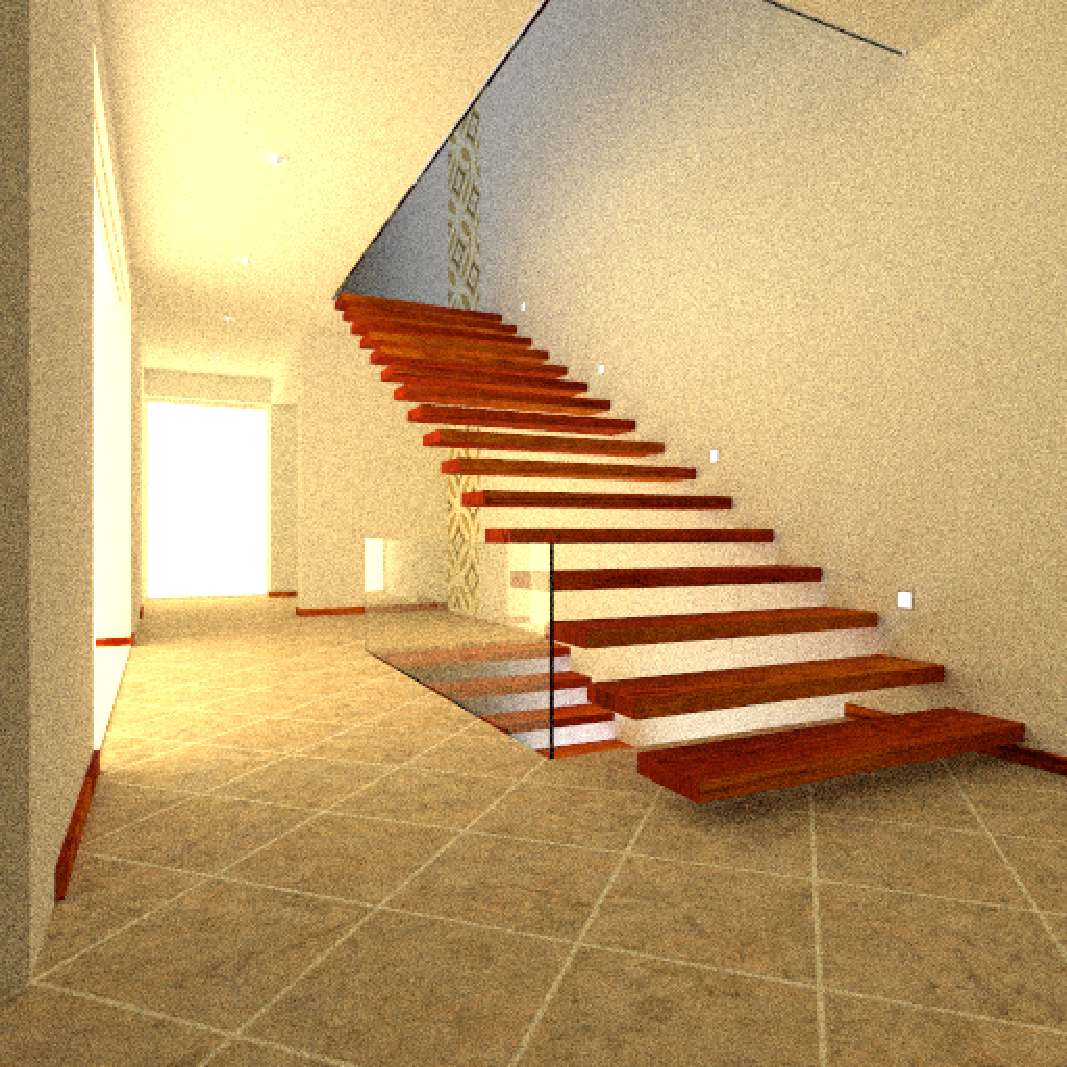
\includegraphics[width=\textwidth]{chapters/chapter_results/correctrender2}
		\caption{Render \texttt{A}}
	\end{subfigure}
	\begin{subfigure}[t]{0.32\linewidth}
		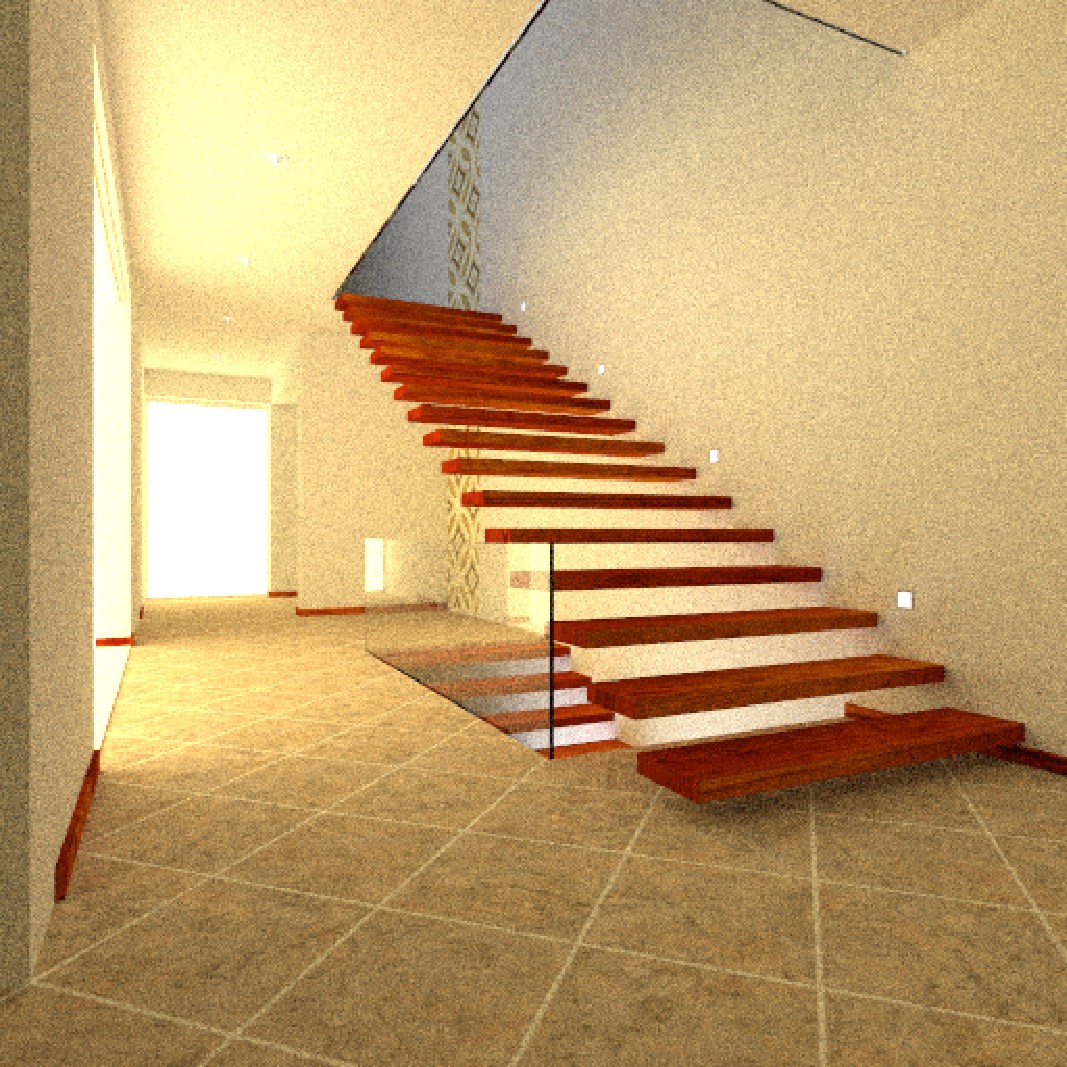
\includegraphics[width=\textwidth]{chapters/chapter_results/wrongrender2}
		\caption{Render \texttt{B}}
	\end{subfigure}
	\begin{subfigure}[t]{0.32\linewidth}
		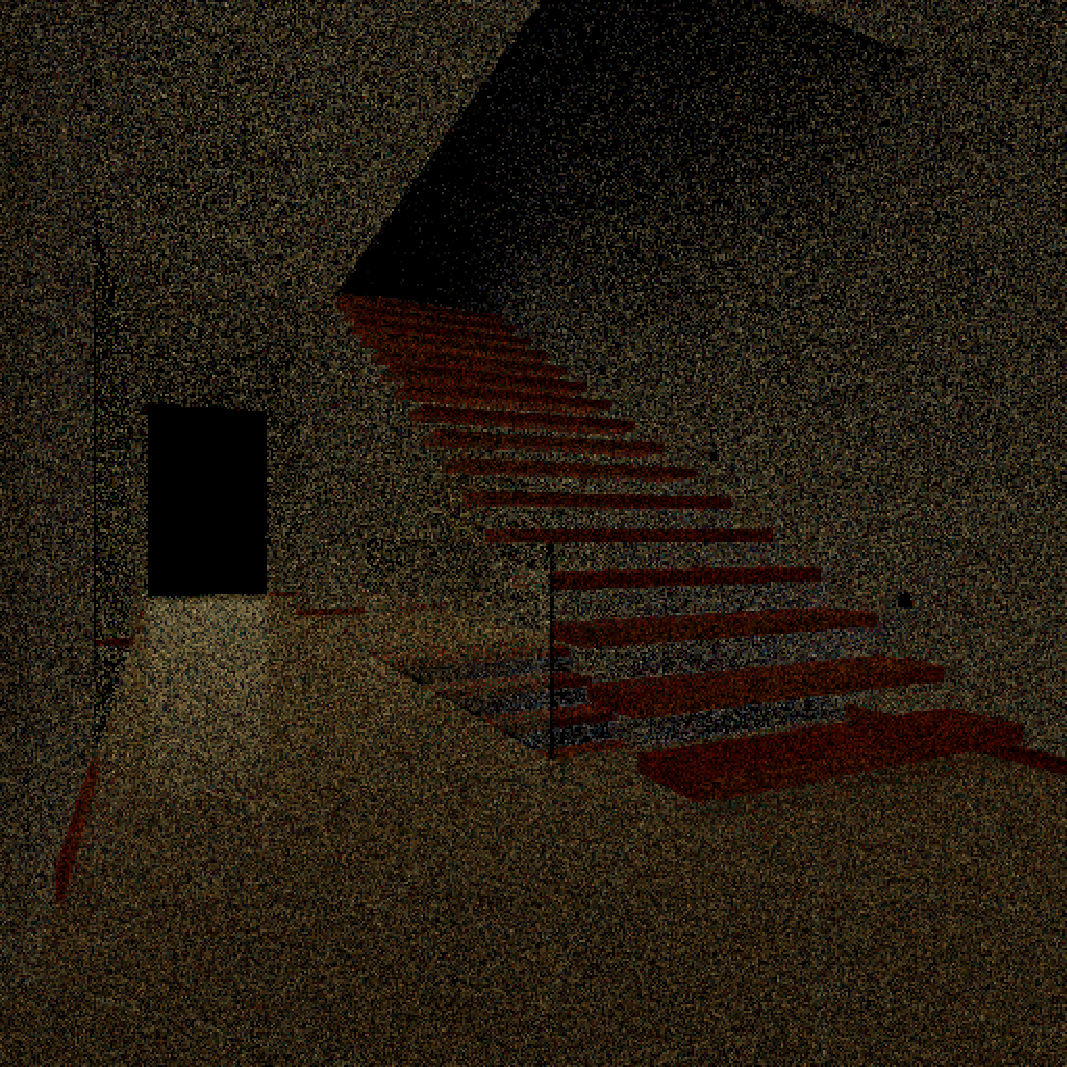
\includegraphics[width=\textwidth]{chapters/chapter_results/render2difference}
		\caption{\texttt{A} $-$ \texttt{B}}
		\label{render2difference}
	\end{subfigure}

	\caption{Render images of the two datasets (\textbf{a}, \textbf{b}) and their mathematical delta (\textbf{c}) to show their differences. (\textbf{c}) has been generated outside the tool and presented for clarity.}
	\label{couple2render}
\end{figure}

To provide a more challenging test, the datasets of which renders are shown in figure \ref{couple2render}, both generated by Yocto/GL \cite{pellacini2019yocto} without multiple importance sampling, have been tinkered to present a very subtle difference. Dataset \texttt{A} is correct while dataset \texttt{B} has been generated after introducing an error in the sampling of microfacet distributions: the direction vector generated according to the distribution has the \textit{y} and \textit{z} components swapped before being transformed from surface space to world space. Logically, this should have generated way more noticeable visual artifacts in the render but, as highlighted by figure \ref{render2difference}, it looks like the wrong render does not account for the Fresnel effect correctly. By just looking at the renders, the user might be led into thinking that there is an error in the Fresnel term calculation or in the surface material in general but here, the situation is different: the direction of the rays are wrong not the calculations of the energy they carry.


\begin{figure}
	\centering
	\begin{subfigure}[t]{0.49\linewidth}
		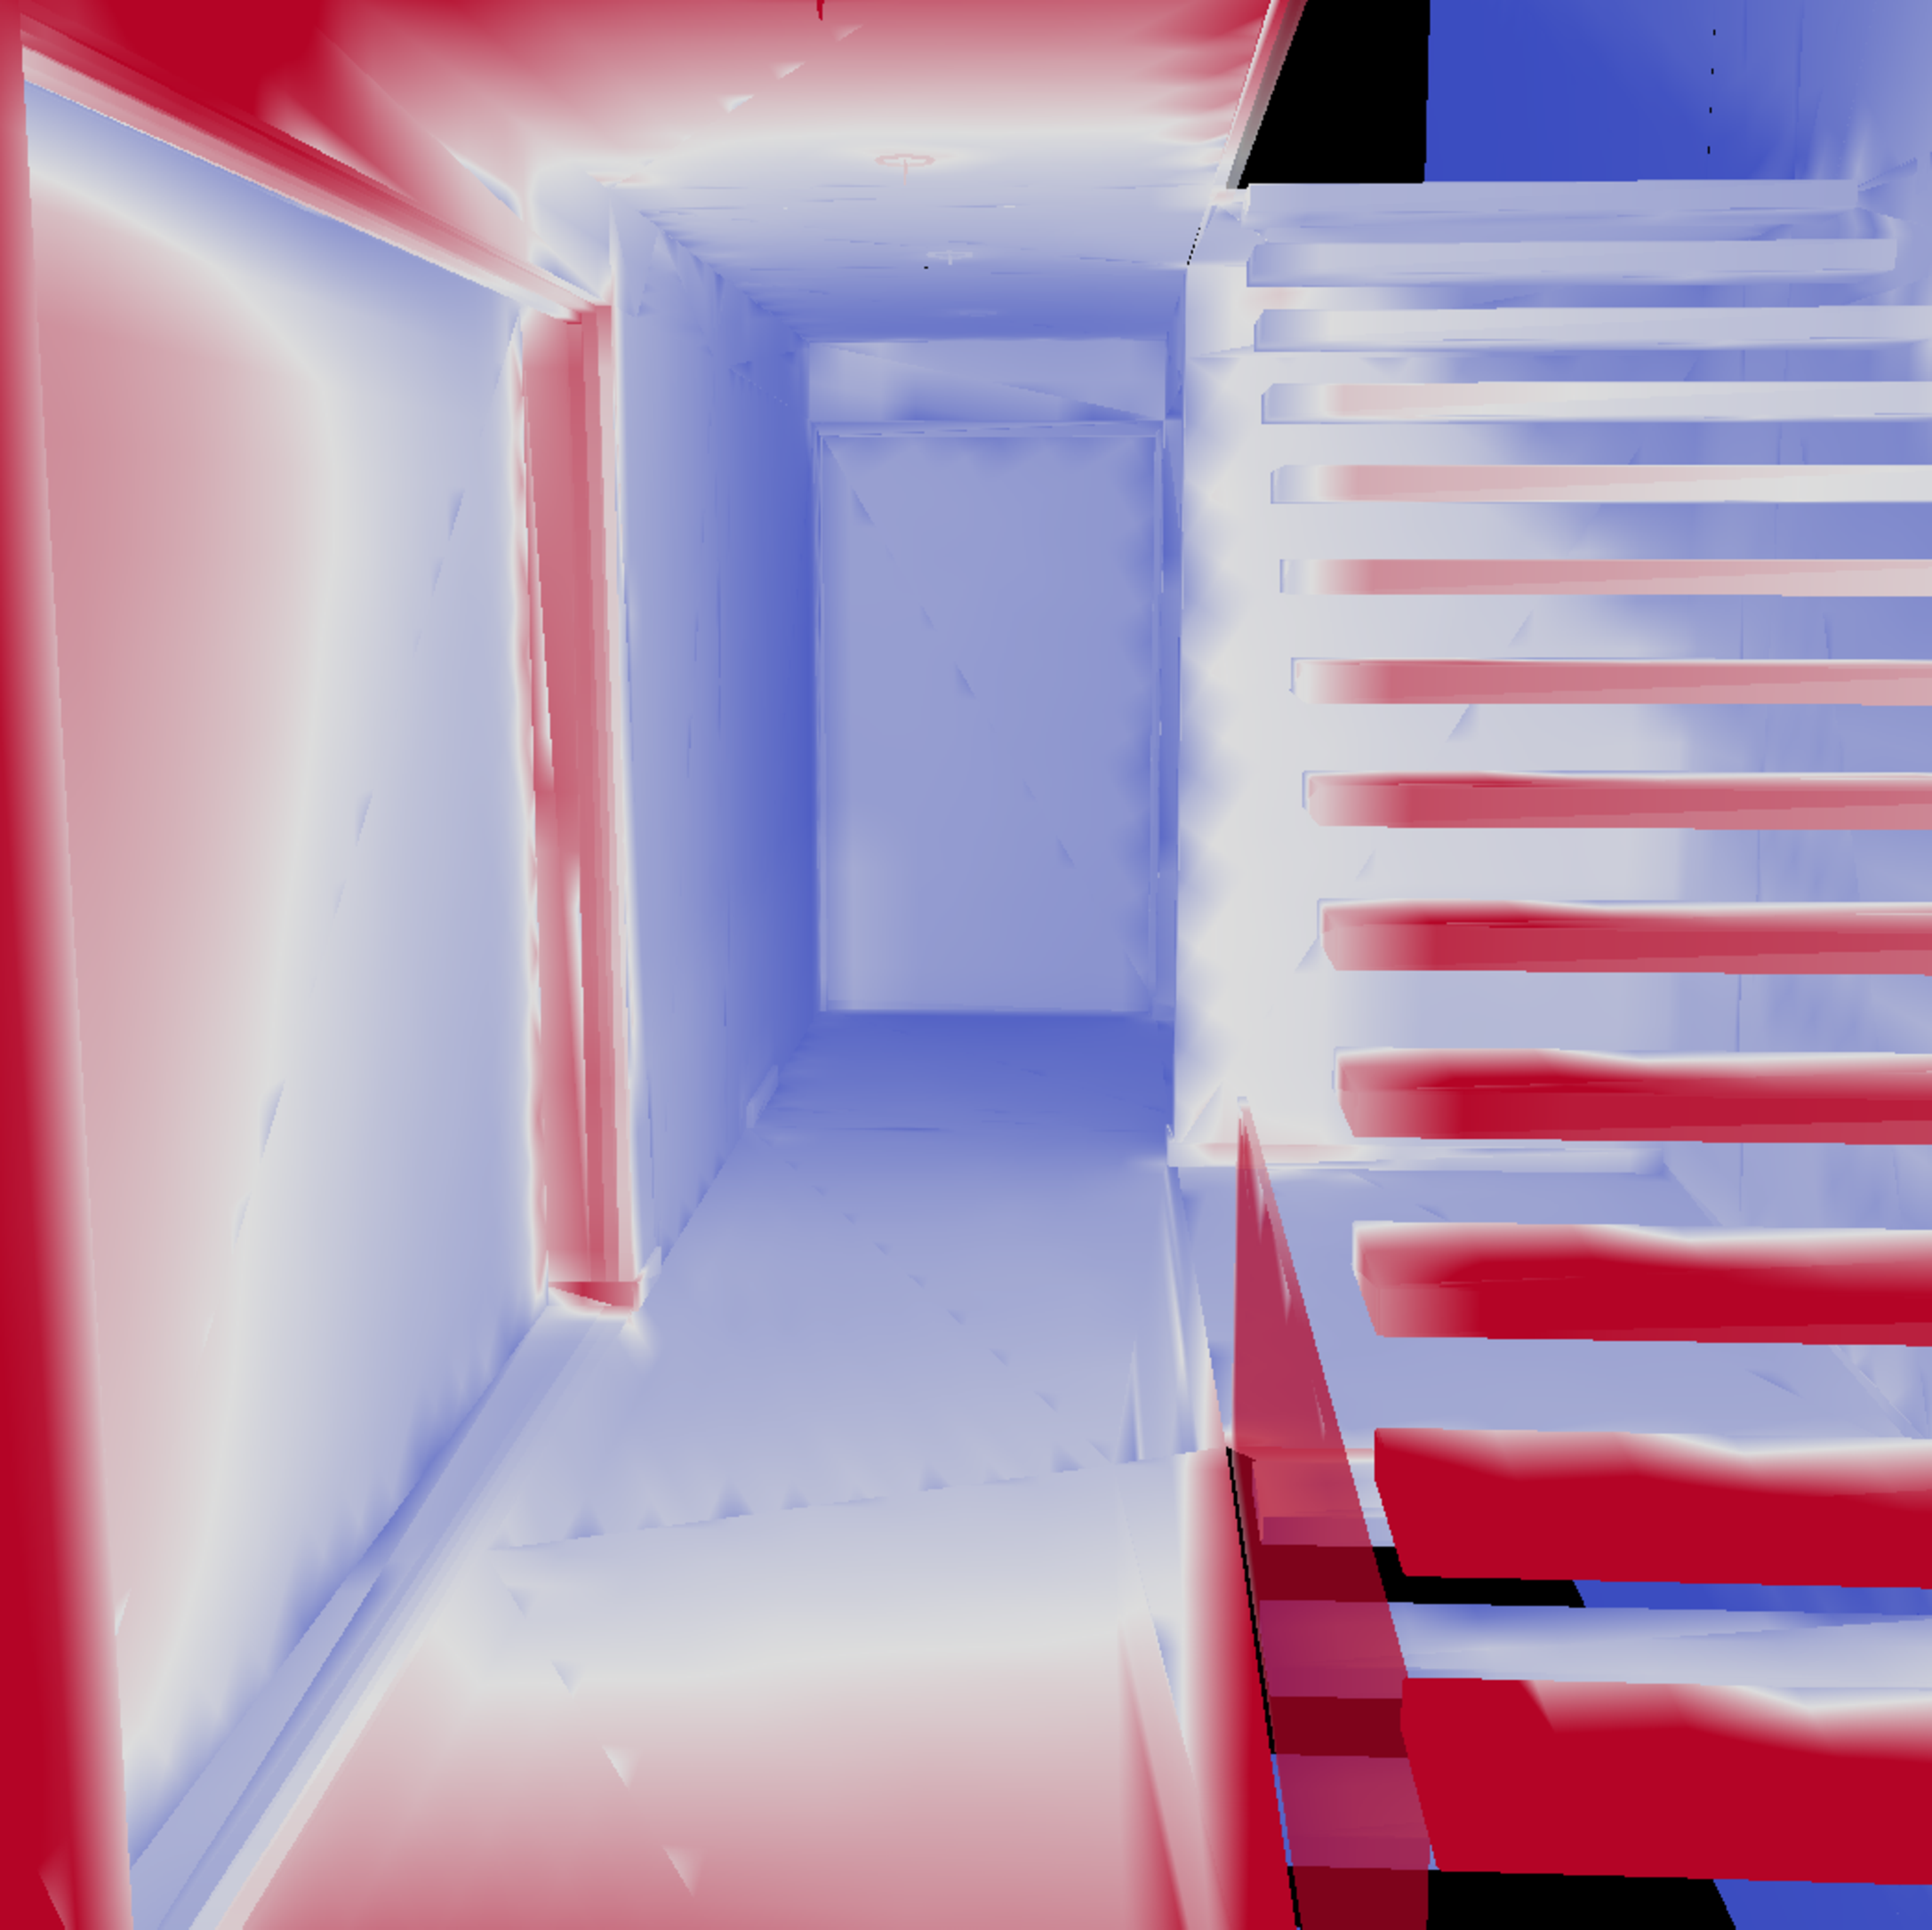
\includegraphics[width=\textwidth]{chapters/chapter_results/correct2heatmap1}
		\caption{Dataset \texttt{A} heatmap 1}
	\end{subfigure}
	\begin{subfigure}[t]{0.49\linewidth}
		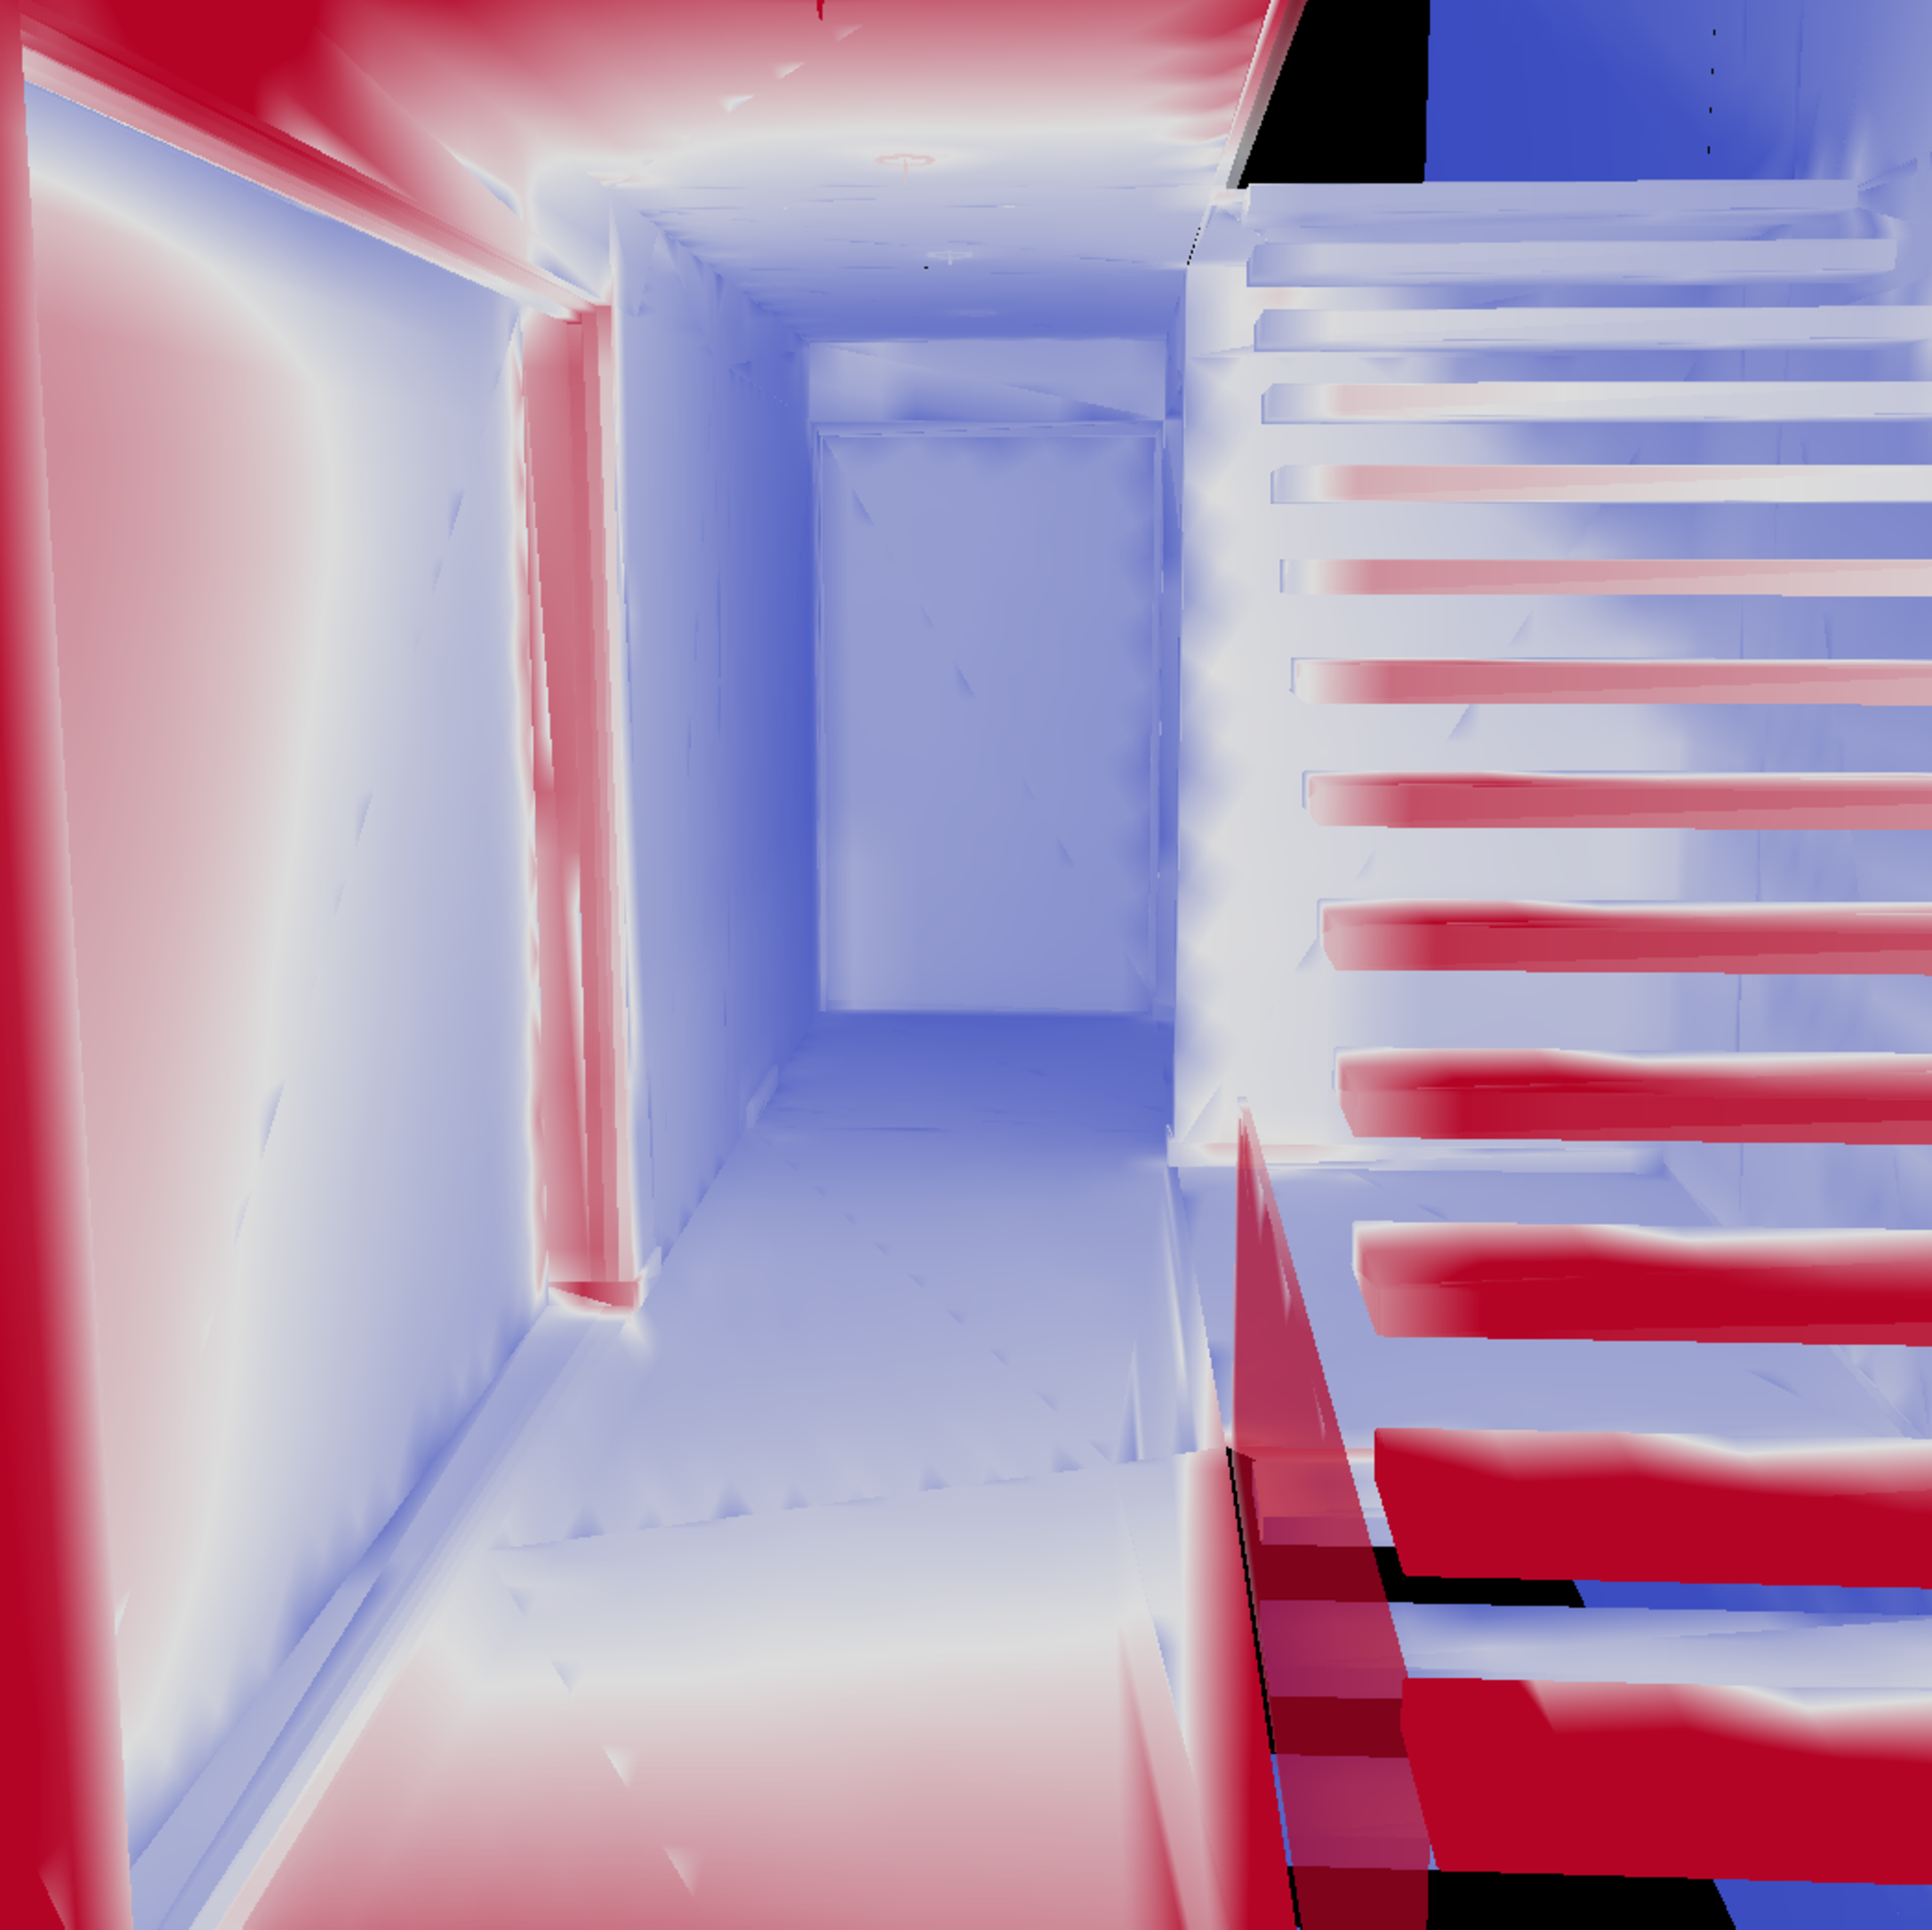
\includegraphics[width=\textwidth]{chapters/chapter_results/wrong2heatmap1}
		\caption{Dataset \texttt{B} heatmap 1}
	\end{subfigure}
	\begin{subfigure}[t]{0.49\linewidth}
		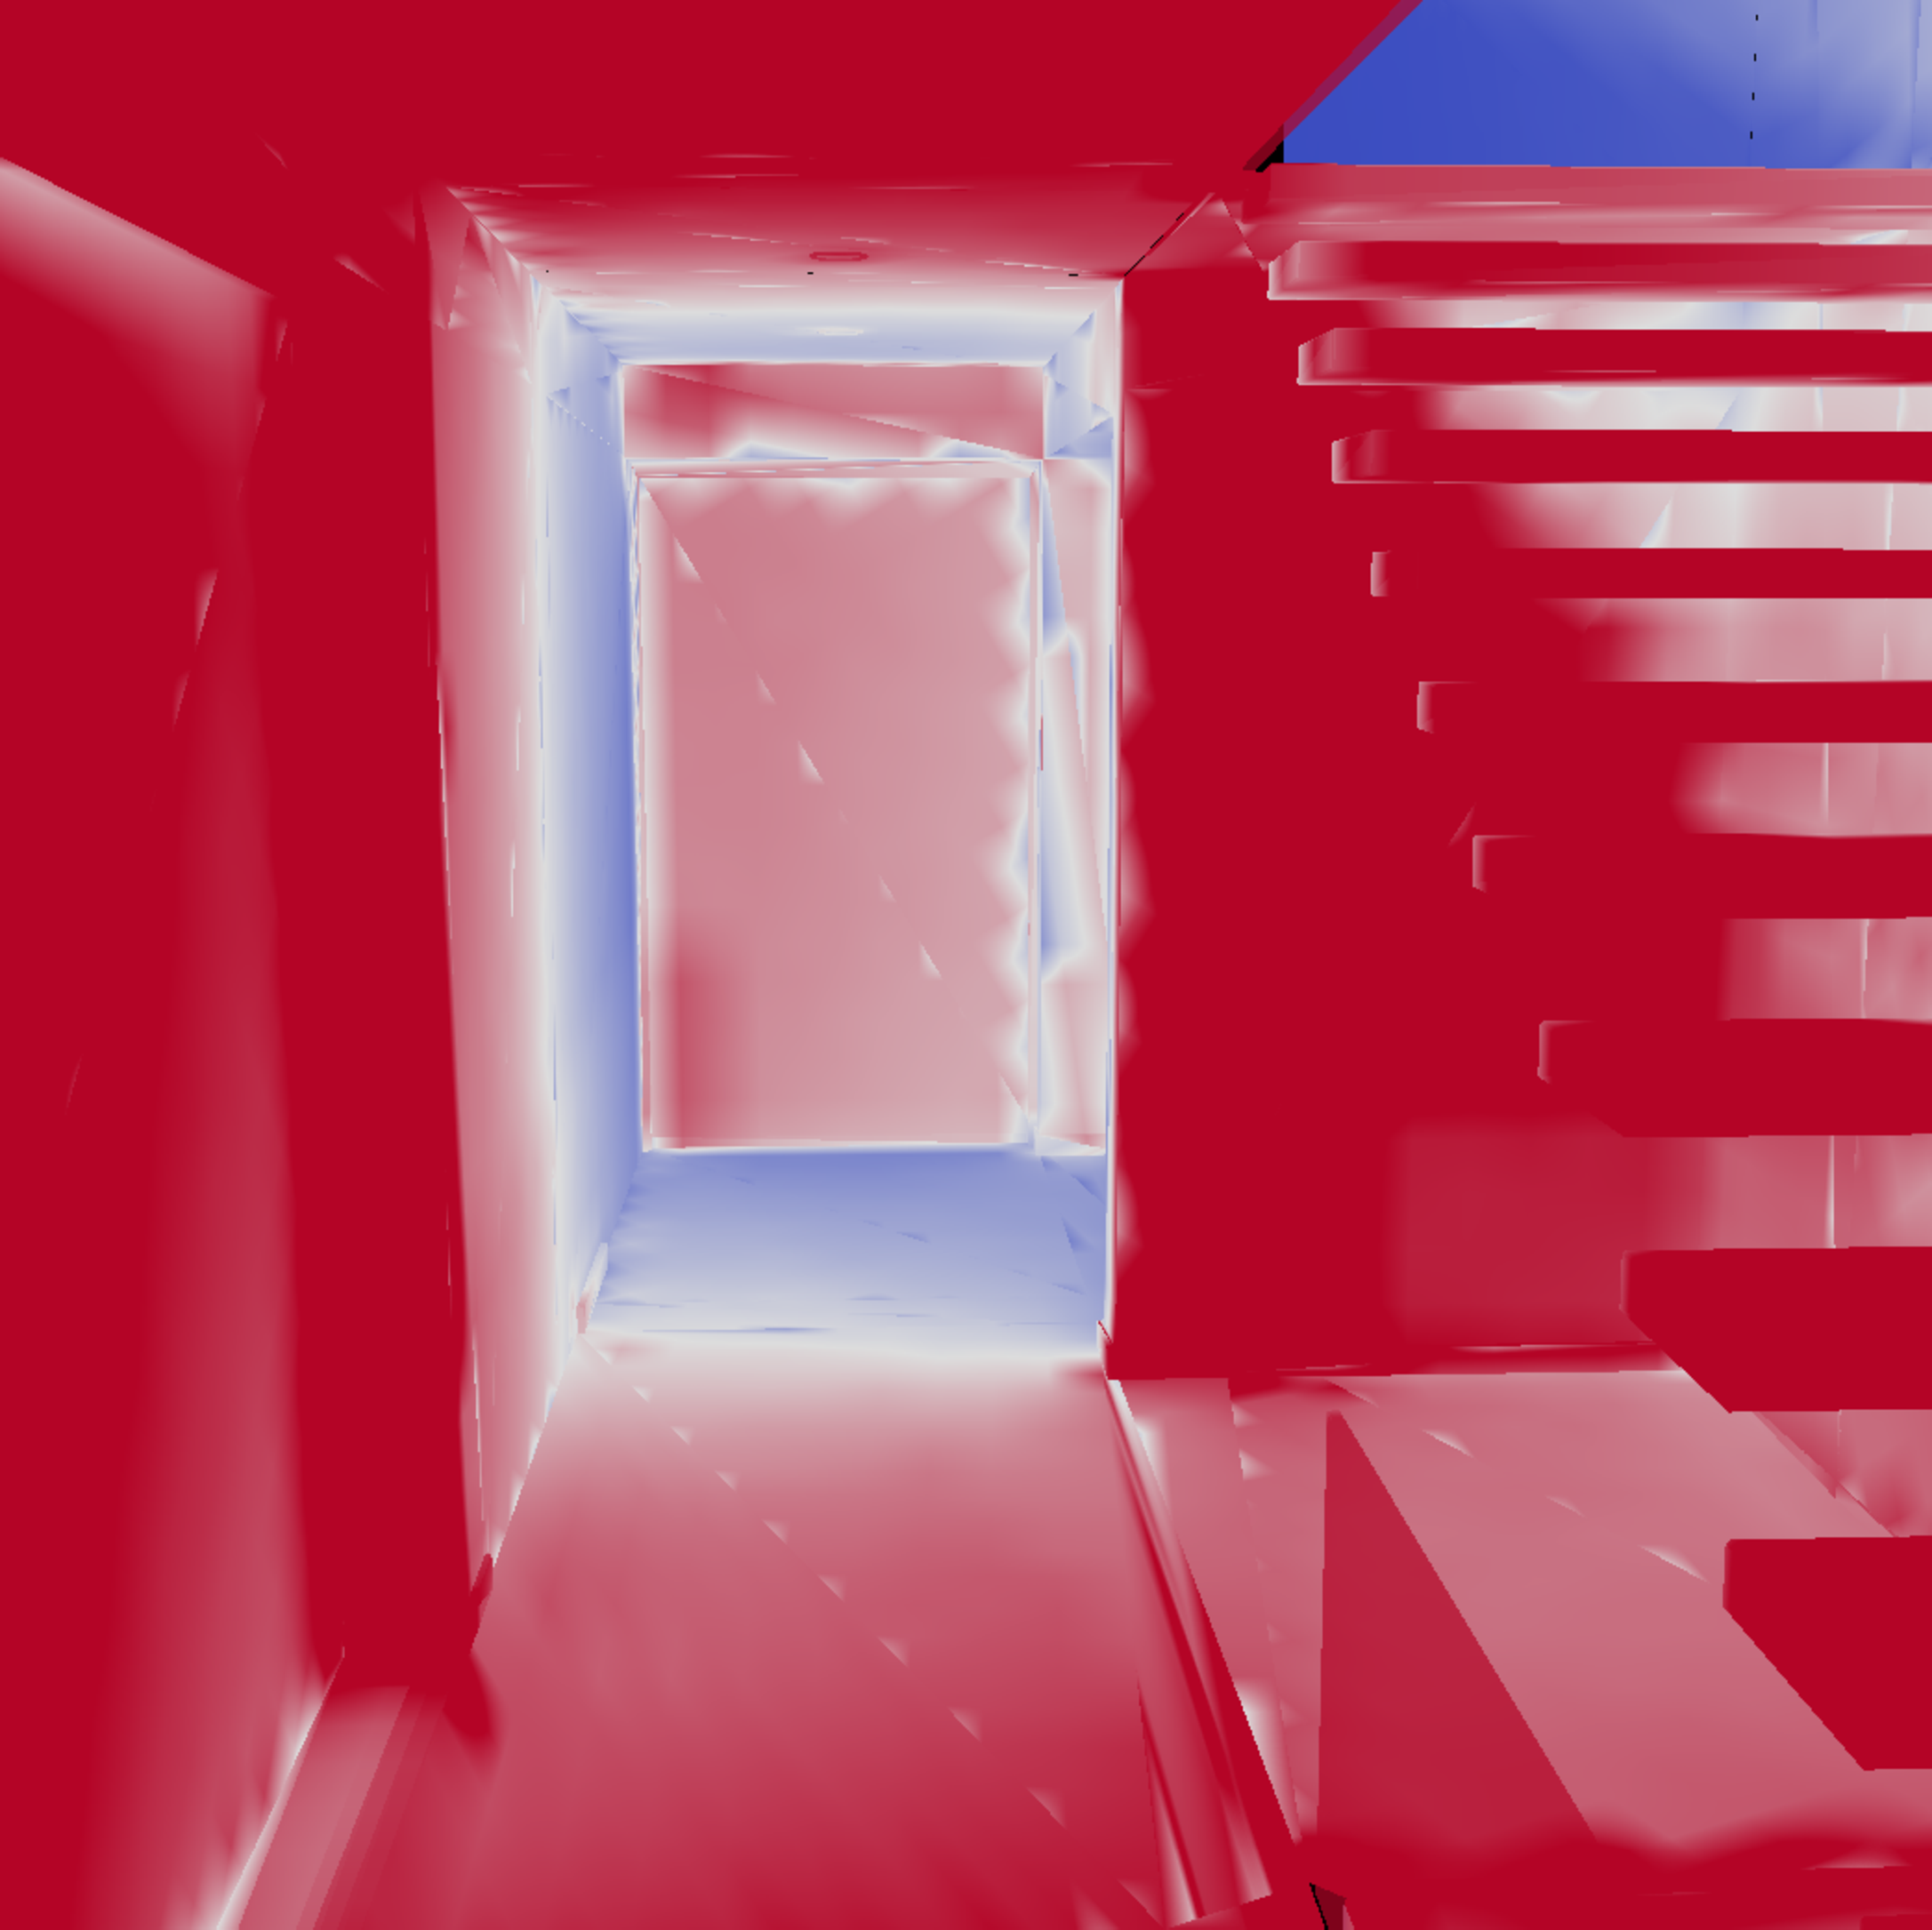
\includegraphics[width=\textwidth]{chapters/chapter_results/correct2heatmap2}
		\caption{Dataset \texttt{A} heatmap 2}
	\end{subfigure}
	\begin{subfigure}[t]{0.49\linewidth}
		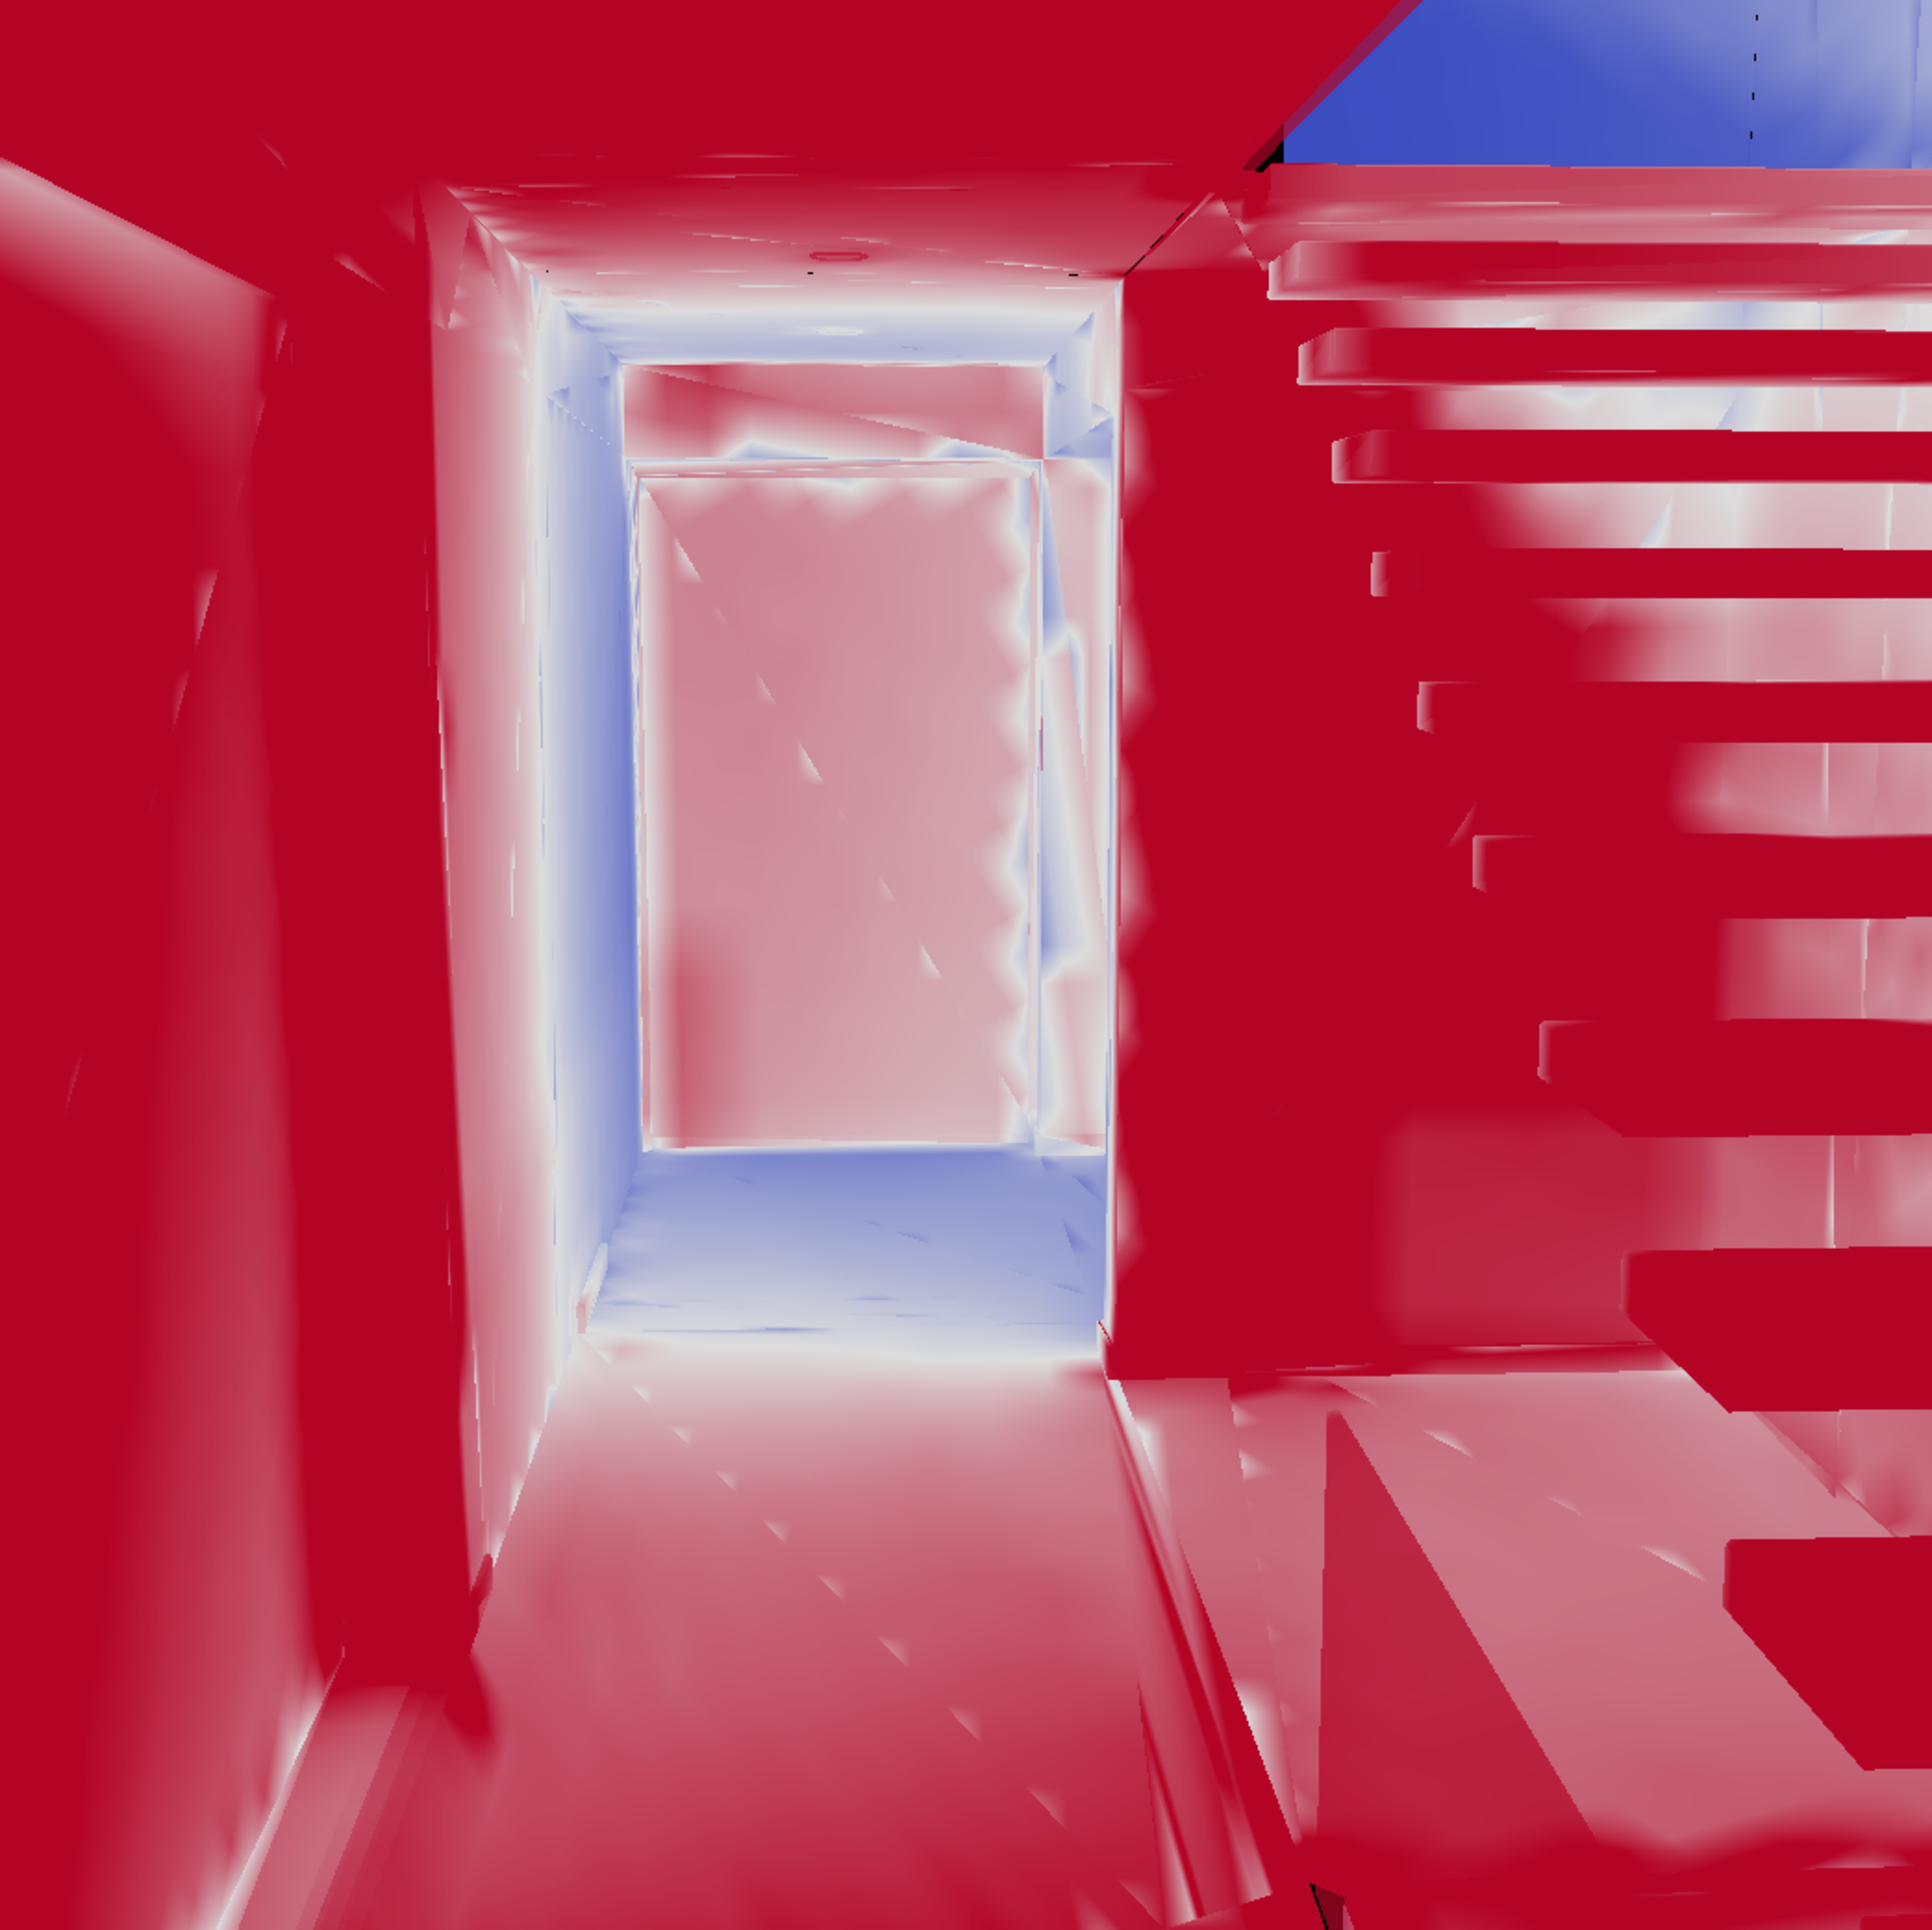
\includegraphics[width=\textwidth]{chapters/chapter_results/wrong2heatmap2}
		\caption{Dataset \texttt{B} heatmap 2}
	\end{subfigure}

	\caption{Heatmap renderings for both datasets from two different cameras and with two different parameters for the \textbf{“Heatmap max”} parameter (for (\textbf{a}) and (\textbf{b}) is set to $100,000$ while for (\textbf{c}) and (\textbf{d}) is set to $40,000$).}
	\label{couple2heatmaps}
\end{figure}

The first instinct was to check the heatmap on the areas where the renders are most different --- that is to say the floor right in front of the light portal at the end of the corridor --- but only minimal differences can be spotted. In the screenshots in figure \ref{couple2heatmaps} vague changes can be seen with a lot of effort, and they just achieve to communicate that the correct dataset --- dataset \texttt{A} --- has a slightly higher bounces density than the wrong dataset. No conclusions can be deducted from this little information.

\begin{figure}
	\centering
	\begin{subfigure}[t]{0.32\linewidth}
		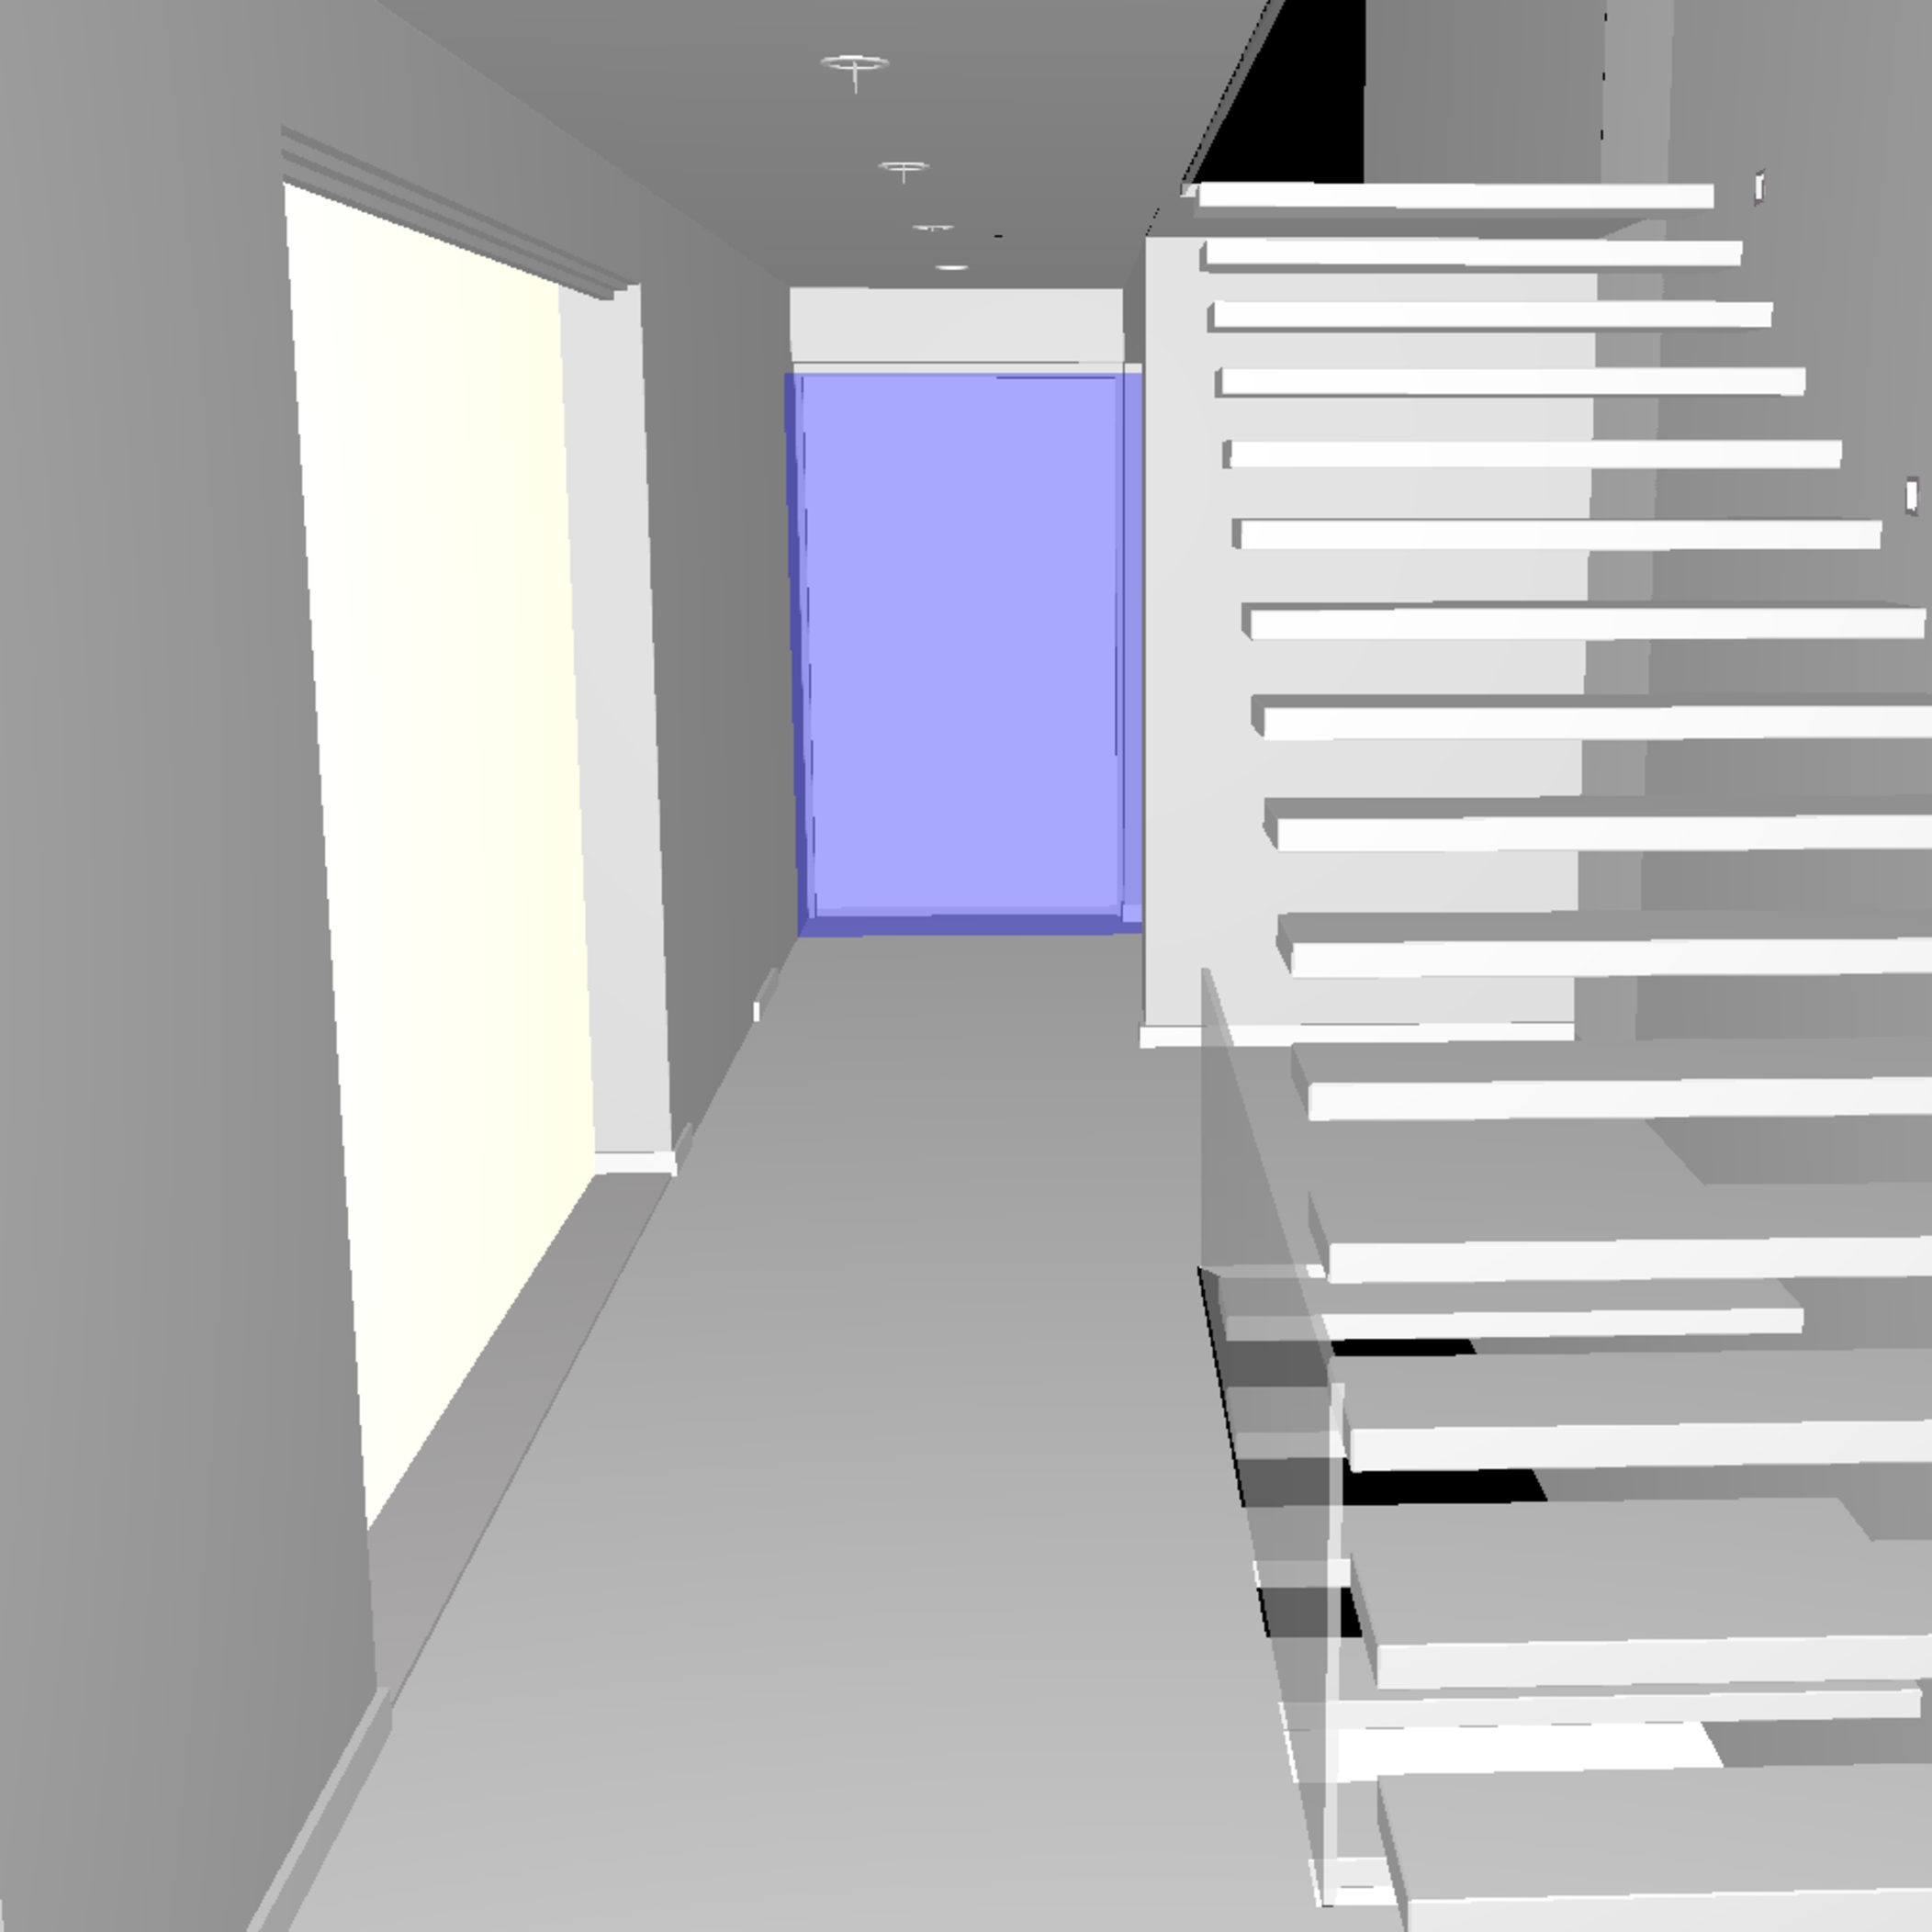
\includegraphics[width=\textwidth]{chapters/chapter_results/ds2filterpos1}
		\caption{Filter position}
	\end{subfigure}
	\begin{subfigure}[t]{0.32\linewidth}
		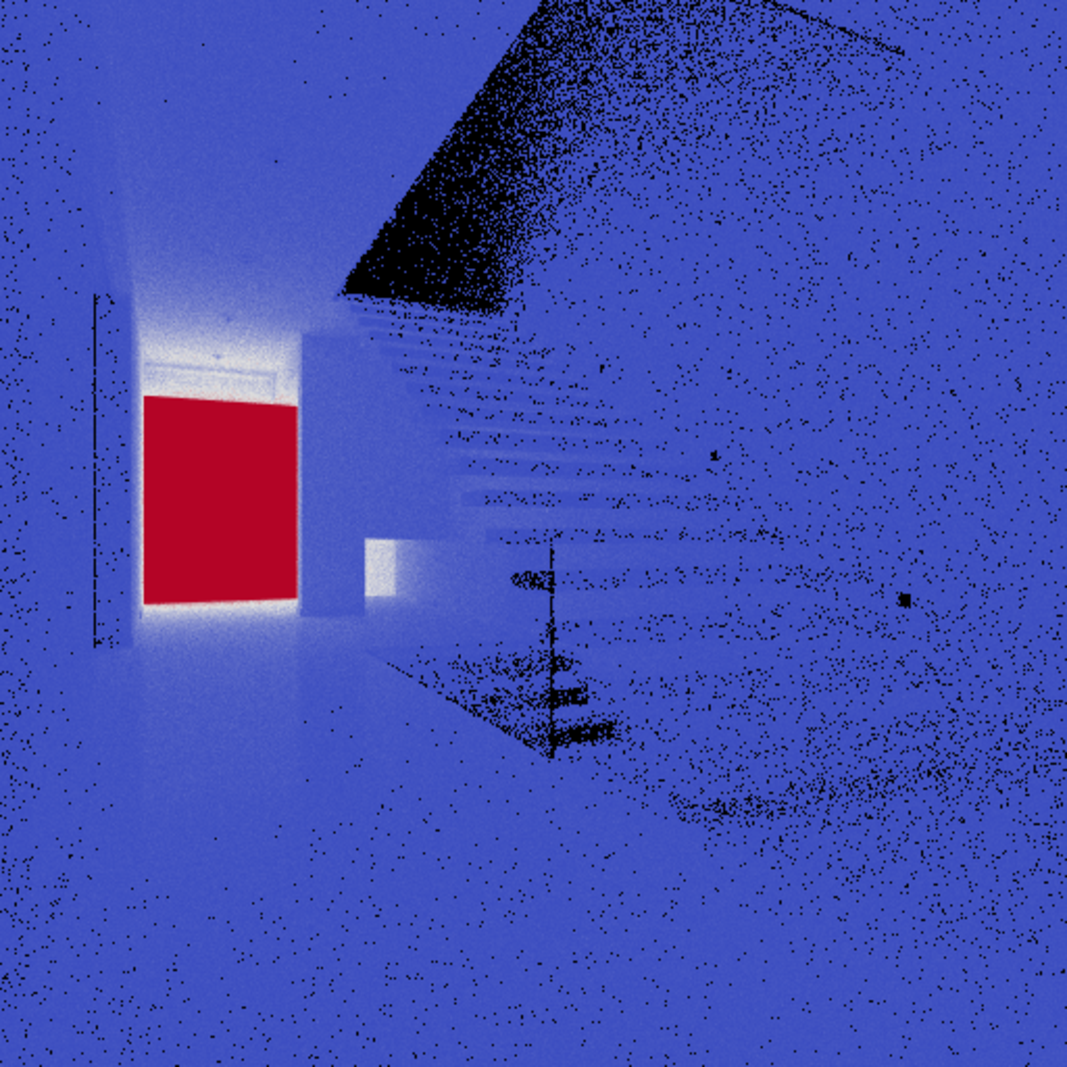
\includegraphics[width=\textwidth]{chapters/chapter_results/correct2ppp}
		\caption{Dataset \texttt{A}}
		\label{correct2ppp}
	\end{subfigure}
	\begin{subfigure}[t]{0.32\linewidth}
		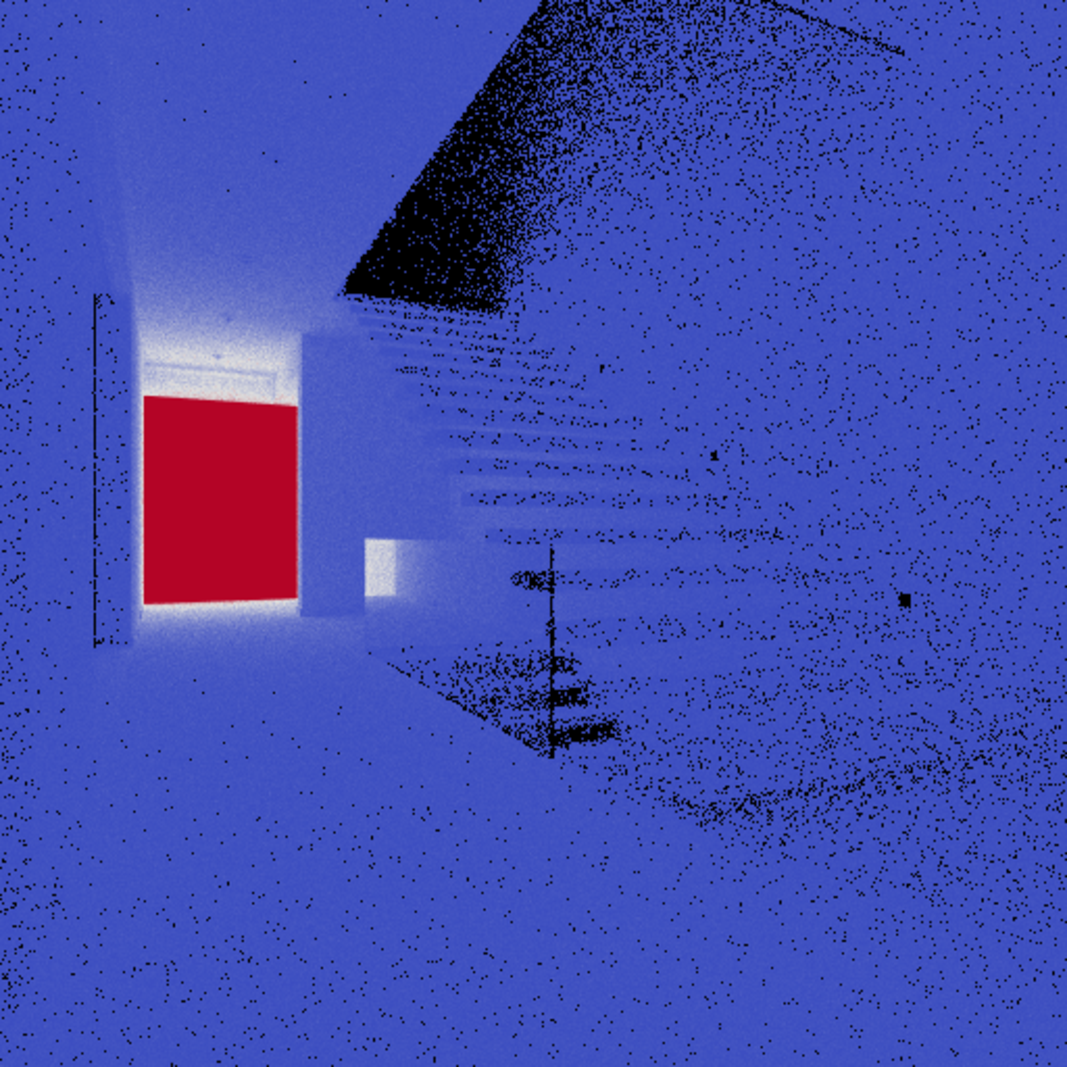
\includegraphics[width=\textwidth]{chapters/chapter_results/wrong2ppp}
		\caption{Dataset \texttt{B}}
		\label{wrong2ppp}
	\end{subfigure}

	\caption{Paths per pixel visualization for the window filter shown in (\textbf{a}).}
	\label{couple2ppp}
\end{figure}

Next step has been to place a window filter covering the entirety of the light at the end of the corridor. Due to the high number of paths selected, the viewport was too visually cluttered to be of any utility, so the focus went on the \textbf{“Render”} panel in the \textbf{“Paths per pixel”} render mode. This, pictured in figures \ref{correct2ppp} and \ref{wrong2ppp}, showed how many more paths in dataset \texttt{A} having their first bounce of the floor ended up hitting that light. It seemed like a further confirmation that something was wrong with the Fresnel term computation.

\begin{figure}
	\centering
	\begin{subfigure}[t]{0.49\linewidth}
		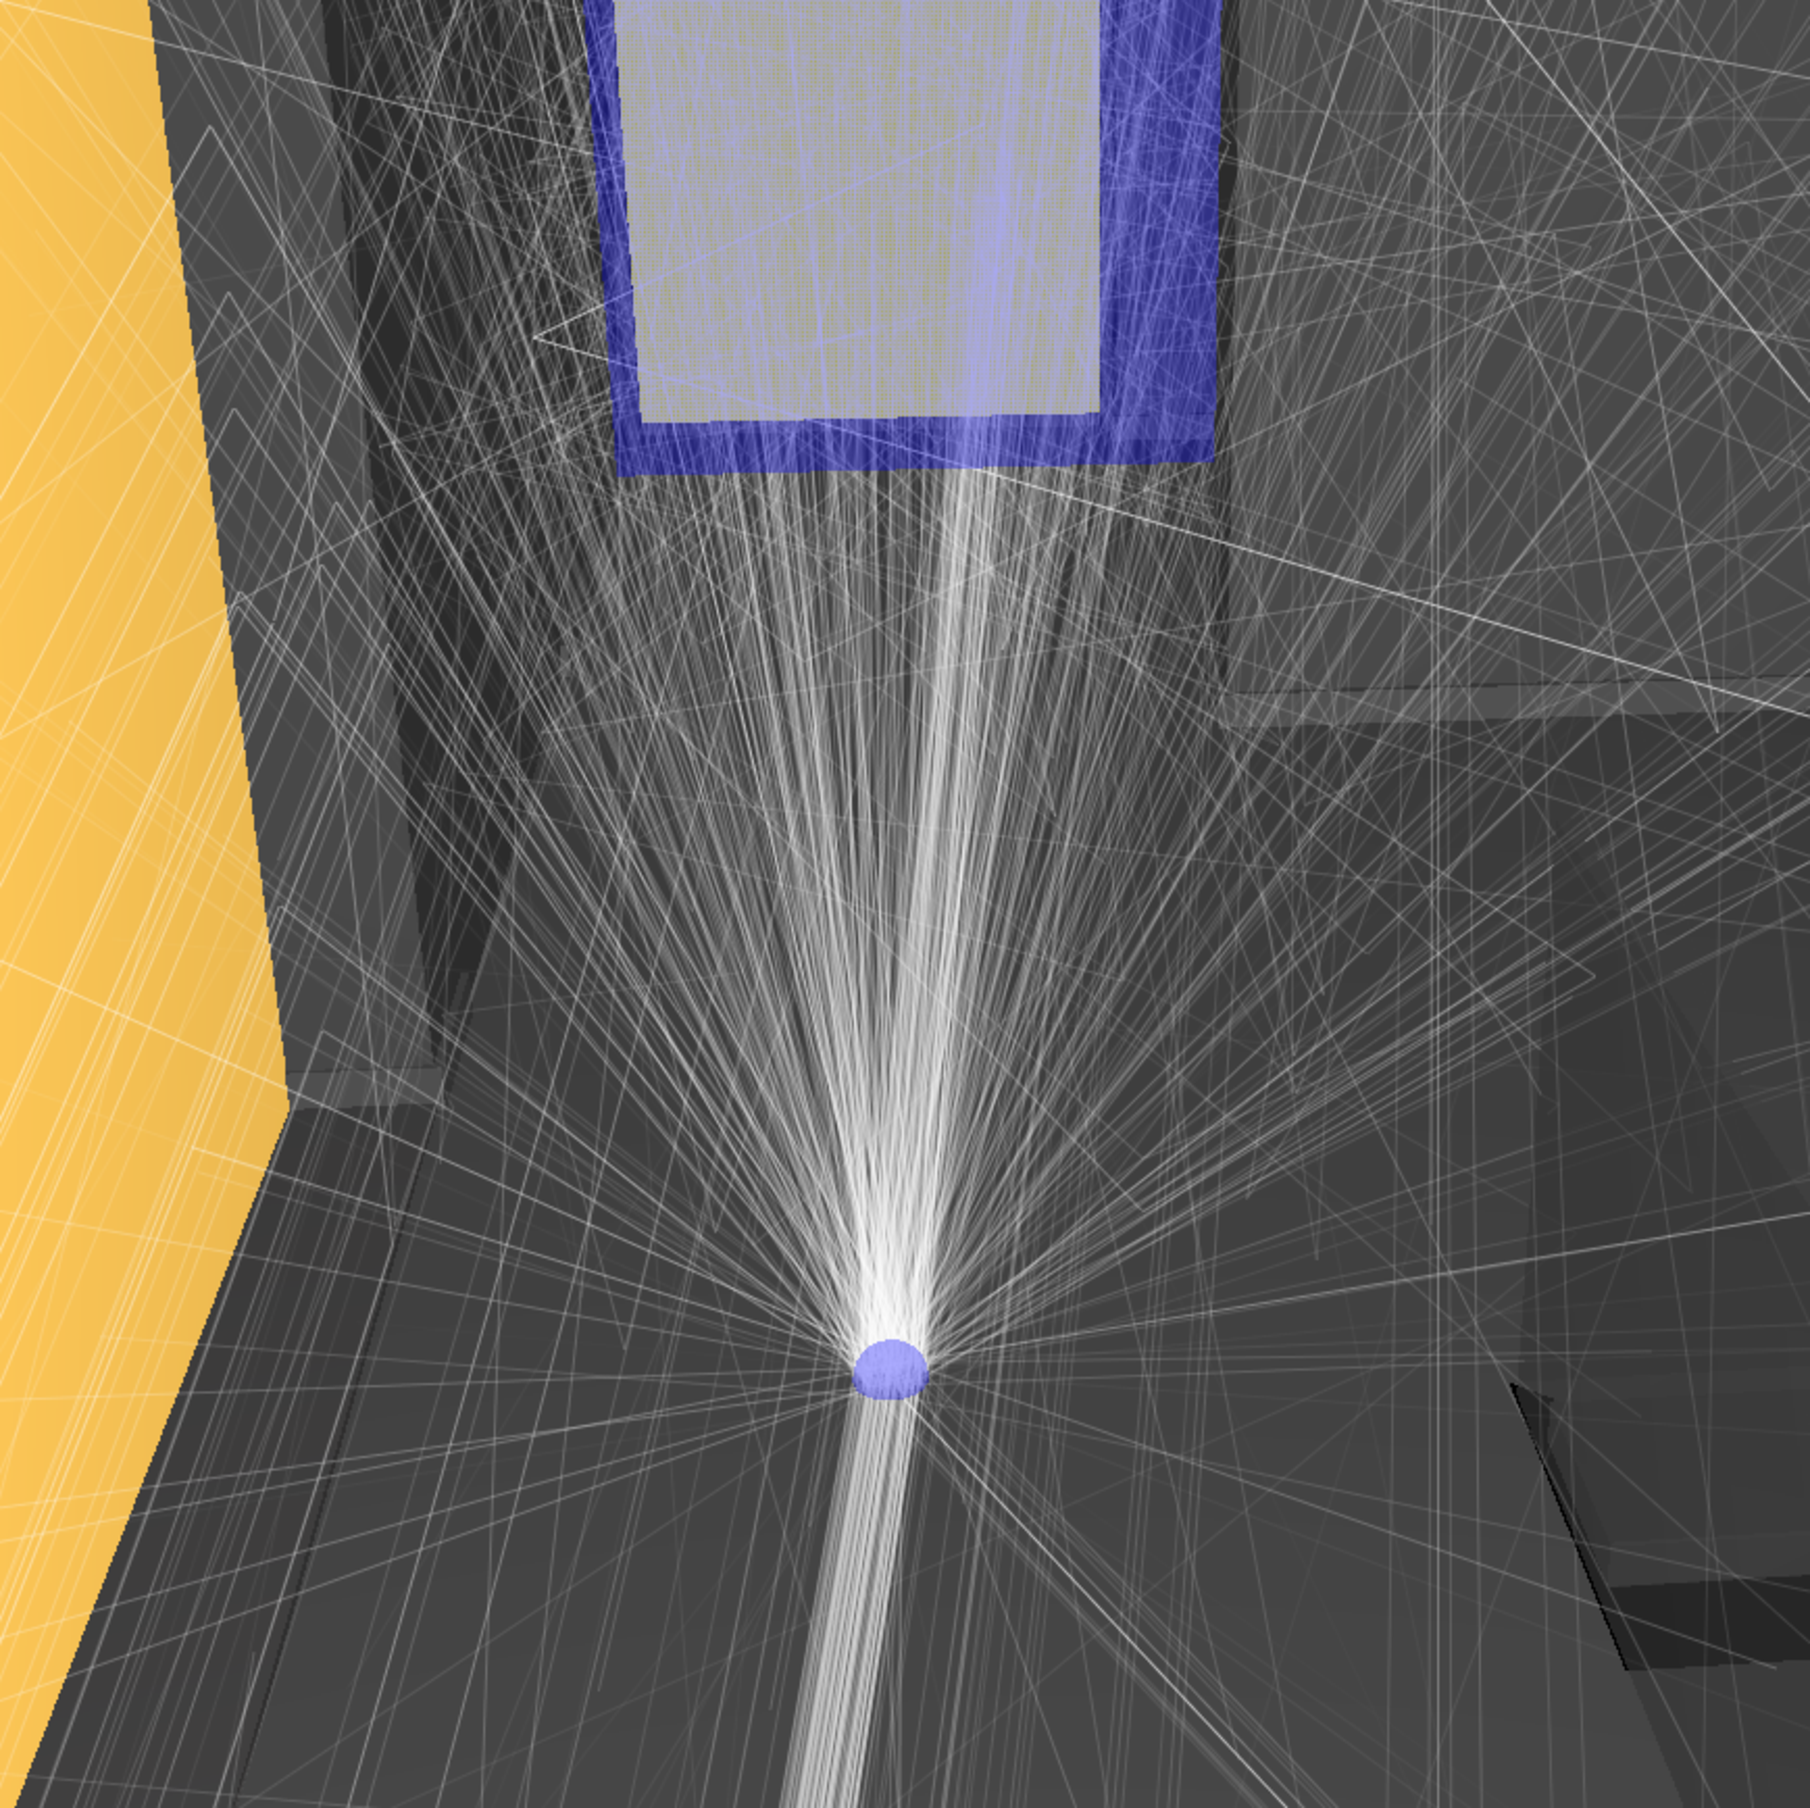
\includegraphics[width=\textwidth]{chapters/chapter_results/correct2pathsscaled}
		\caption{\texttt{A}, radiance scaled}
		\label{correct2pathsscaled}
	\end{subfigure}
	\begin{subfigure}[t]{0.49\linewidth}
		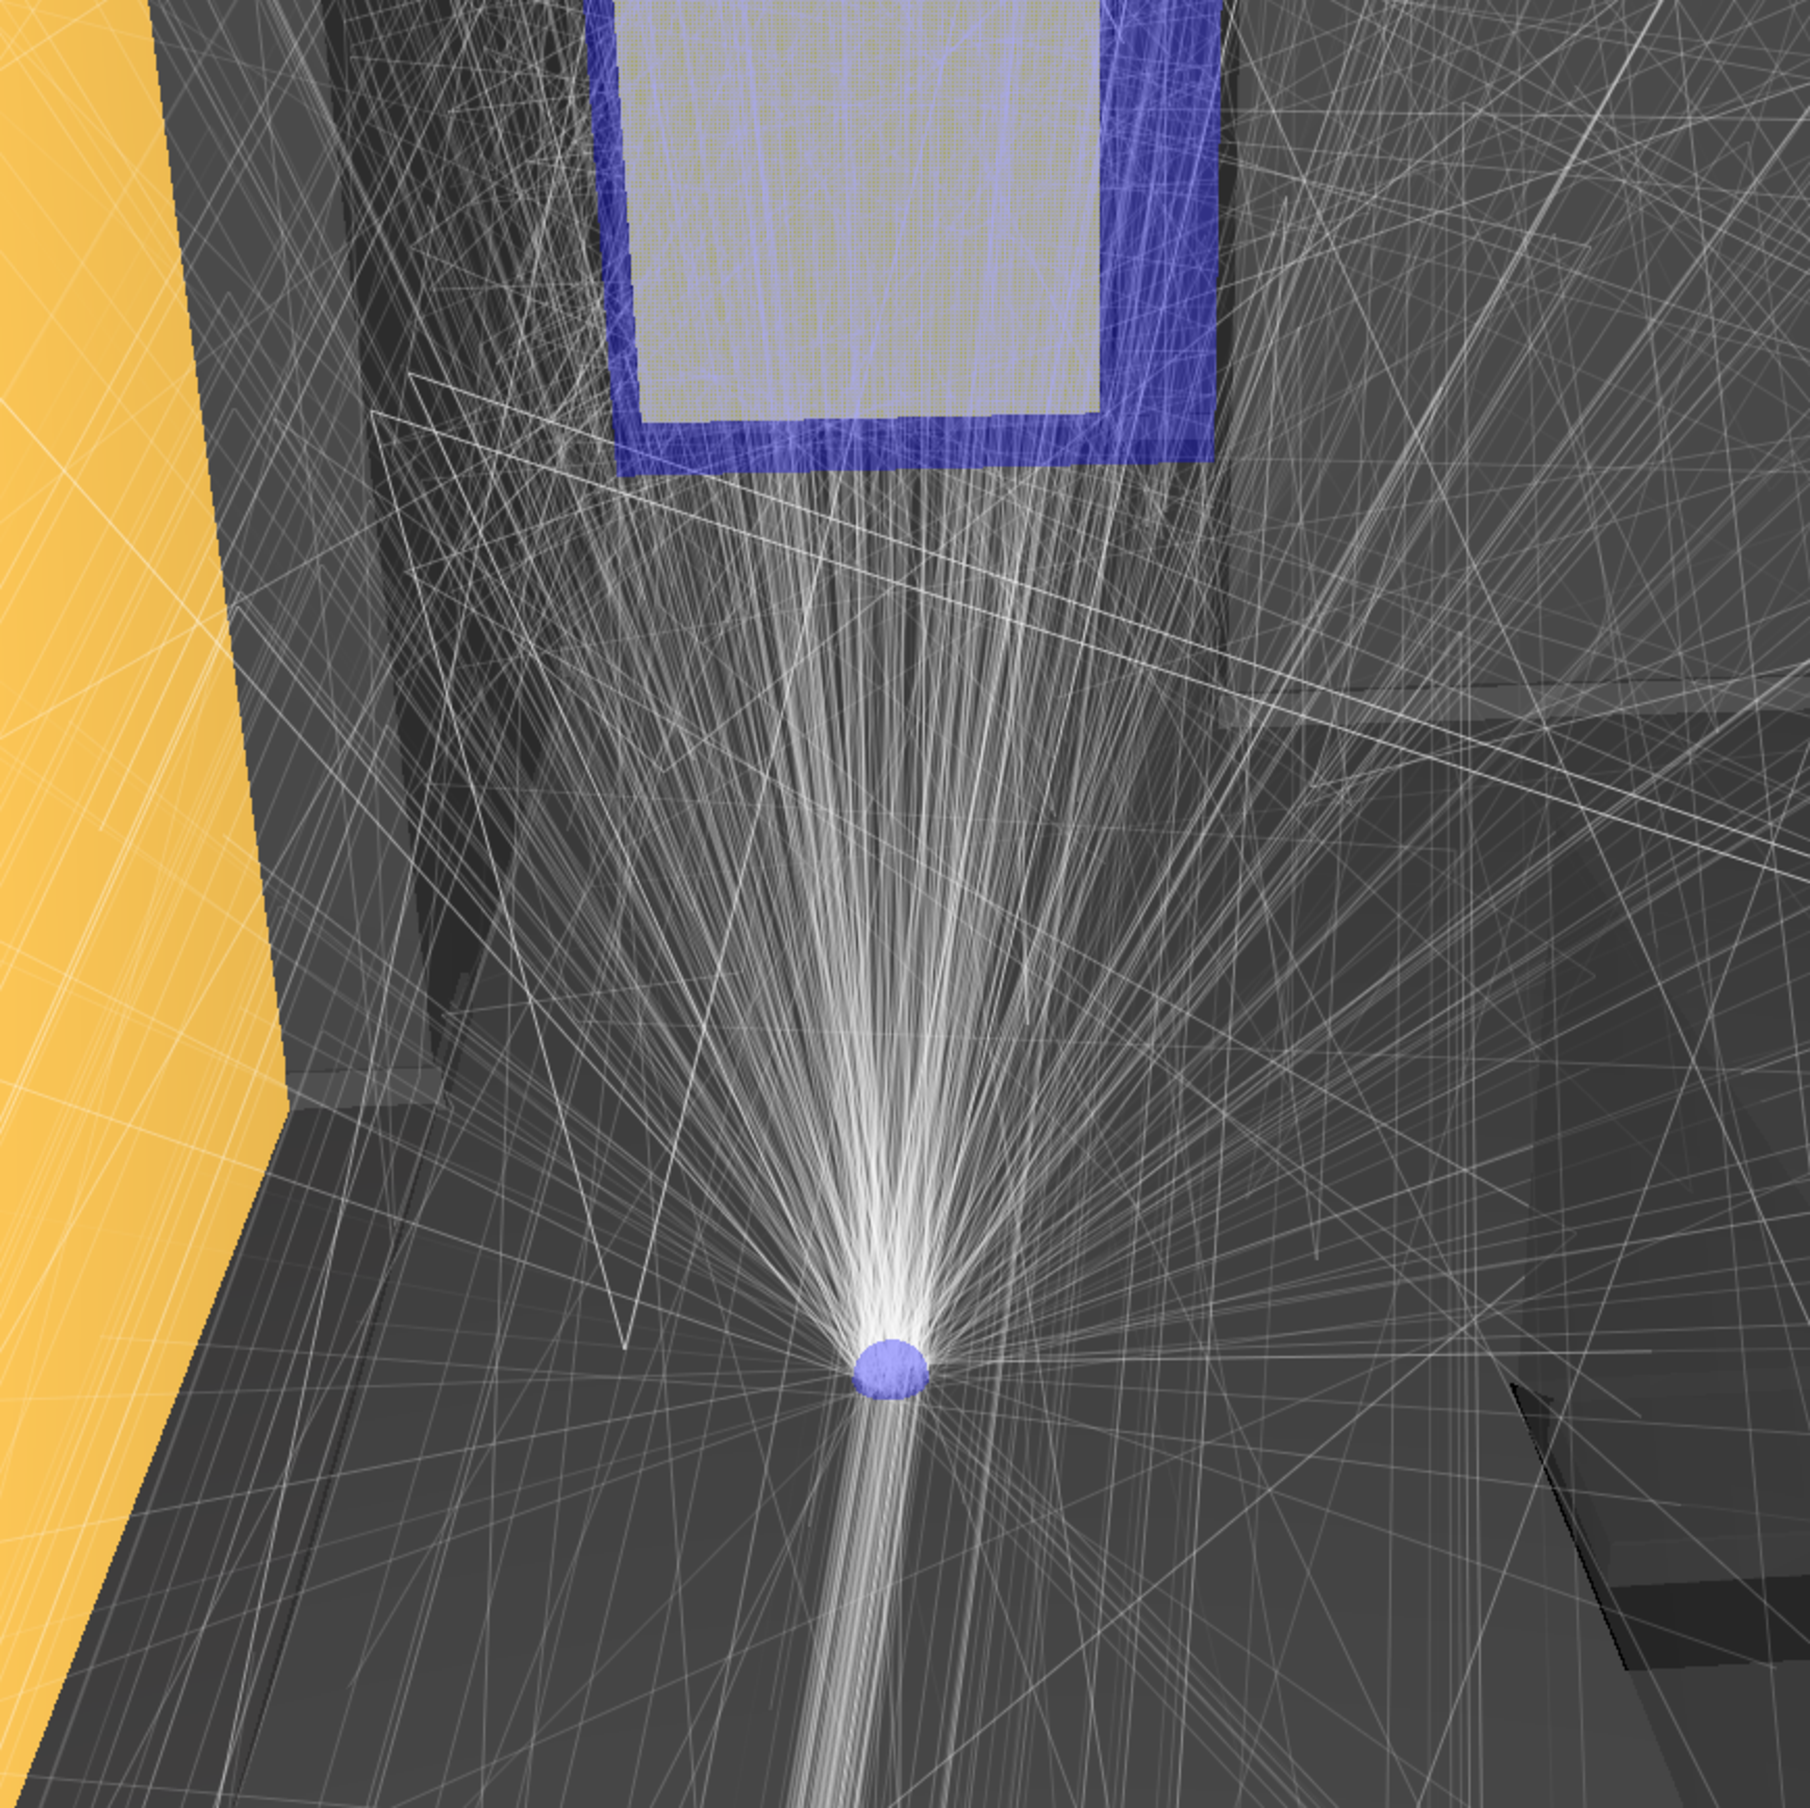
\includegraphics[width=\textwidth]{chapters/chapter_results/wrong2pathsscaled}
		\caption{\texttt{B}, radiance scaled}
		\label{wrong2pathsscaled}
	\end{subfigure}
	\begin{subfigure}[t]{0.49\linewidth}
		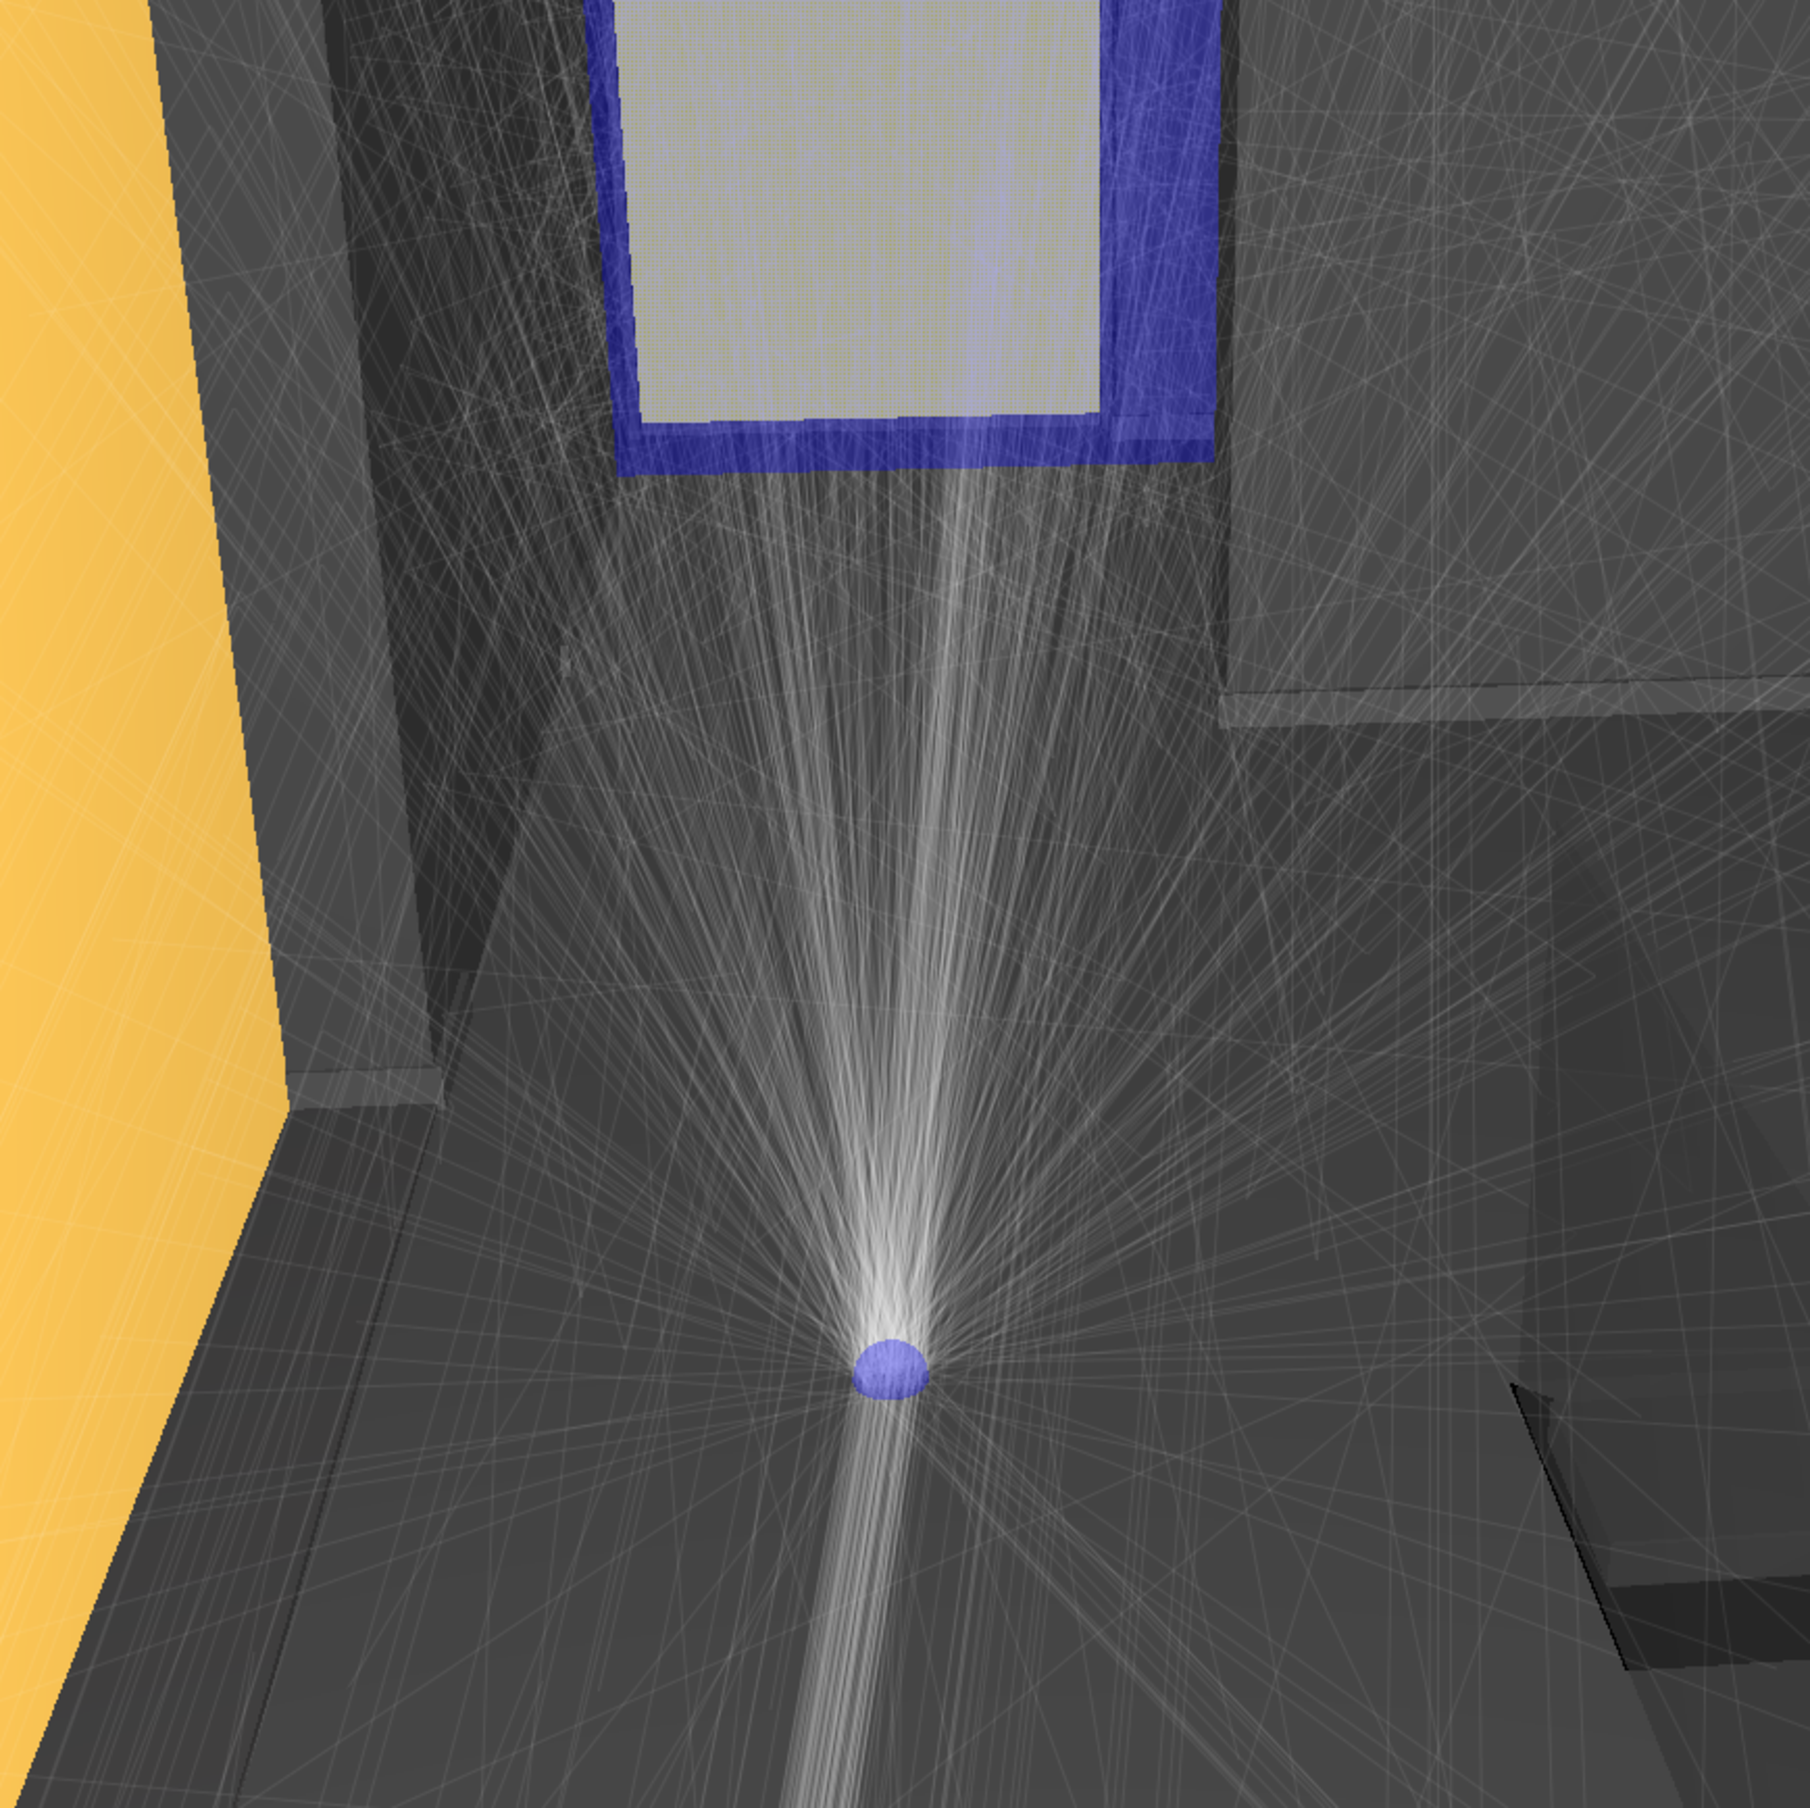
\includegraphics[width=\textwidth]{chapters/chapter_results/correct2paths}
		\caption{\texttt{A}, no radiance scaling}
	\end{subfigure}
	\begin{subfigure}[t]{0.49\linewidth}
		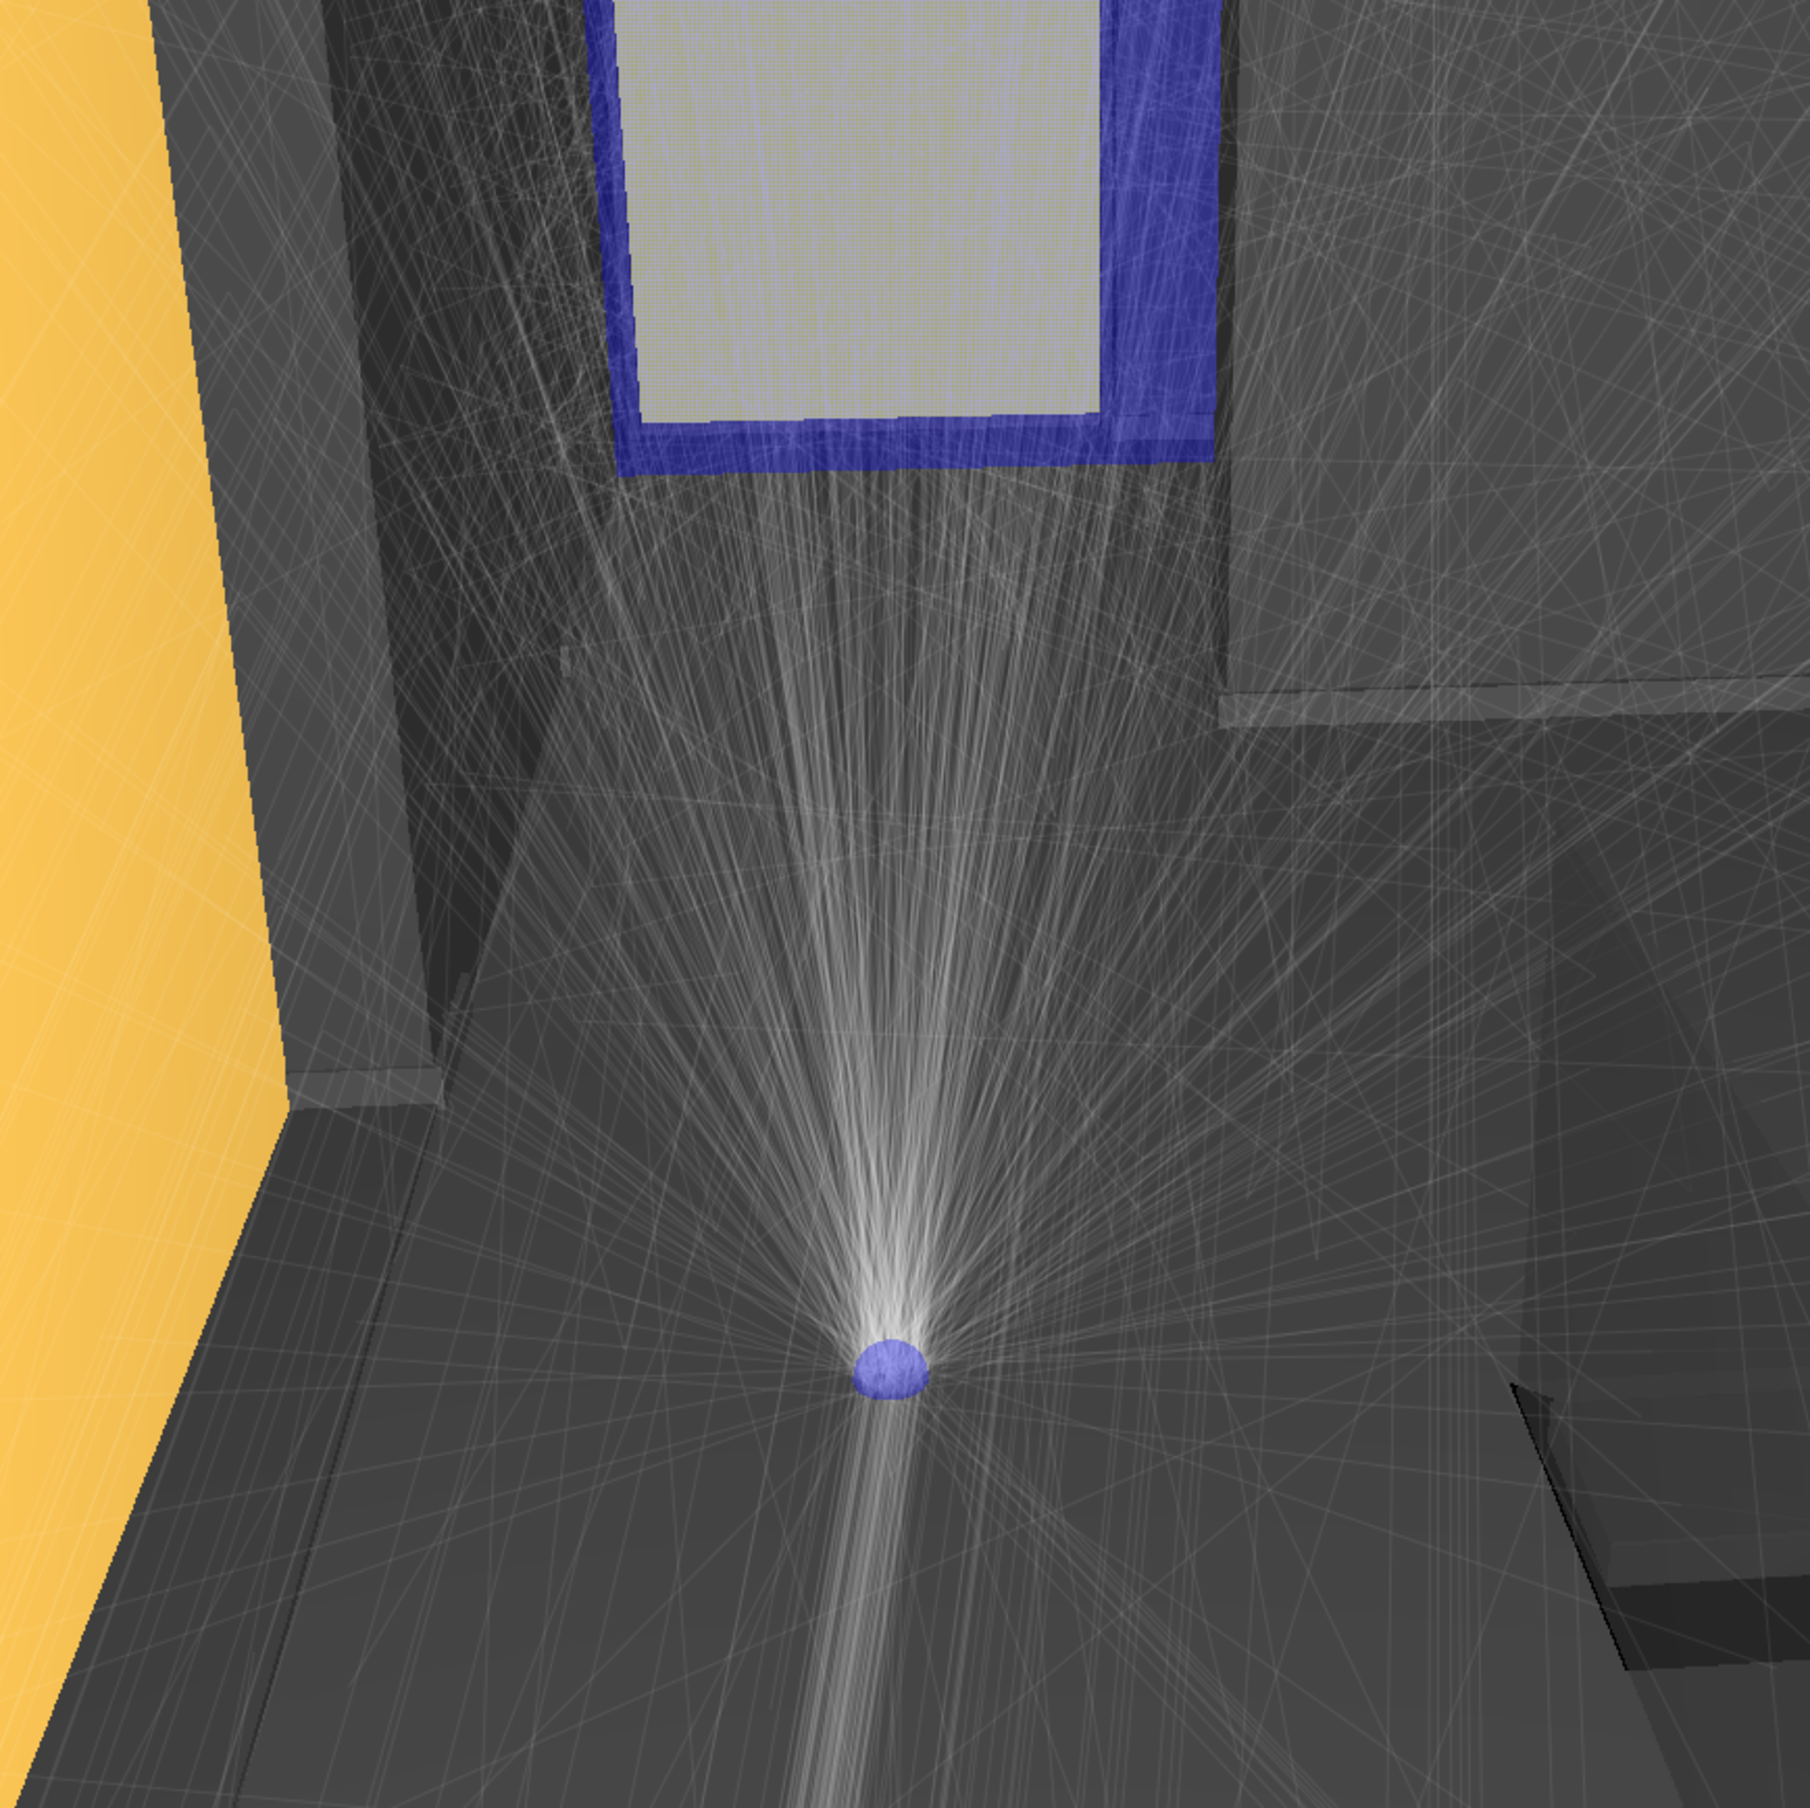
\includegraphics[width=\textwidth]{chapters/chapter_results/wrong2paths}
		\caption{\texttt{B}, no radiance scaling}
	\end{subfigure}

	\caption{Viewport renderings of paths bouncing in the sphere filter placed on the floor and through the window filter on the light in the back. (\textbf{a}) and (\textbf{b}) have the \textbf{“Radiance scaling”} visualization option activated while the others do not. Scene rendering has been darkened using the tool's visualization options.}
	\label{couple2paths}
\end{figure}

It all seemed even further confirmed by placing a sphere filter on the floor where the Fresnel effect shows and analyzing the geometry of paths through there. As shown in figure \ref{couple2paths}, a clear bundle of rays going from the sphere to the window filter appears for dataset \texttt{A}, but not for dataset \texttt{B}. When only looking at those paths having the \textbf{“Radiance scaling”} visualization option activated (fig. \ref{correct2pathsscaled} and \ref{wrong2pathsscaled}), the theory about the error in the Fresnel term computation  might still stand strong; after all, due to the high quantity of paths displayed, it is difficult to understand if that bundle of rays is there in both datasets but it carries way less radiance in dataset \texttt{B} due to miscalculations while evaluating the material.

All doubts are dispelled by disabling the \textbf{“Radiance scaling”}. As soon as it is off, it is clear that that bundle of rays is there, no matter the energy it carries. It shows that the problem is in the picking of a new ray direction that, even if strictly related to surface material evaluation, it is still not in the Fresnel term evaluation.

This conclusion, even if correct, has been drawn by taking several steps in a direction probably dictated by our previous knowledge of the bug. We do not know and cannot make estimates on how any different user would approach the debugging process having this tool available. Nevertheless, this example would fit way more in an educational context as much as the previous did: it could be used to show in a visual way the crucial importance of correct next event estimation since it does not only affect the convergence times --- so how much noise ends up being in the final image --- but also the \textit{correctness} of the render process.